\label{ch:tf}

% Describe how this Ch is organized
This chapter examines the applicability of machine learning to capture the behavior of an experiment during the transient provided its thermal properties are known.
Data-based modeling, which relies on machine learning, extracts features from data generated with the physics-based model and predicts the behavior of new data.
Hence, a thermal-fluids solver is necessary to determine the thermal behavior of the experiment and generate the required data to train and test the data-based model.
Section \ref{sec:tf} describes the thermal-fluids solvers utilized in this work.
Additionally, this work compares the performance of different data-based strategies.
Section \ref{sec:ML} introduces briefly the machine learning algorithms utilized in this work, Section \ref{sec:simpl-model} introduces a simplified thermal-fluids model, its verification, and it investigates the performance of the different data-based approaches and machine learning algorithms.
Section \ref{sec:datapros} discusses some necessary changes in the data processing to implement the data-based modeling for an experiment subject to delayed heating.
Finally, Section \ref{sec:atr} demonstrates the data-based modeling of an ATR experiment undergoing the accident.


\section{Thermal-Fluids Solvers}
\label{sec:tf}

\subsection{MOOSE}

% fairhurst-agosta_machine_2_2022
The \gls*{MOOSE} \cite{gaston_moose_2009}, originally released in 2008, is an open-source \gls*{FEM} framework that supports engineering analysis applications, targeting systems of non-linear partial differential equations.
The MOOSE applications define weak forms of the governing equations and modularize the physics expressions into \textit{kernels}.
The kernels are C++ classes containing methods for computing the residual and Jacobian contributions of individual pieces of the governing equations.
All the software built on the MOOSE framework shares the same \gls*{API}.
This feature facilitates a relatively easy coupling between different phenomena.
Additionally, the framework and its applications use \gls*{MPI} for parallel communication and can be deployed on massively parallel cluster-computing platforms.

% MOOSE role in the calculations
In this work, MOOSE solves a simplified thermal-fluids model (Section \ref{sec:simpl-model}) to examine the applicability of machine learning to capture the experiment thermal behavior.
Three reasons motivated the choice of MOOSE for such a study.
First, the author's familiarity with the software made it the natural choice.
% Second, the MOOSE input sequence consists of only one script, while OpenFOAM’s comprises several scripts.
Second, the MOOSE input sequence consists of only one script, which reduces the burden of handling a large number of files.
Third, the MOOSE model uses the Boussinesq approximation to reduce the computational expense of the simulation.
The approximation considers that the density-variation effects are only present in the body force term of the conservation of momentum equations.
% MOOSE / Equations
% fairhurst-agosta_machine_2_2022
This approximation reduces the system of equations in the fluid region to three equations for solving the motion and temperature
% Equations
\begin{align}
& \nabla \cdot \vec{u} = 0 \\
& \rho \left( \frac{\partial \vec{u}}{\partial t} + (\vec{u} \cdot \nabla)\vec{u} \right) + \nabla p - \rho \vec{g} + \rho \vec{g} \beta (T - T_{ref}) - \mu \Delta \vec{u}= 0 \\
& \rho c_p \left( \frac{\partial T}{\partial t} + (\vec{u} \cdot \nabla) T \right) - k \Delta T - q''' = 0  
\end{align}
where $\vec{u}$ is the velocity, $\rho$ is the density, $p$ is the pressure, $\vec{g}$ is the gravity, $\beta$ is the thermal expansion coefficient, $T$ is the temperature, $T_{ref}$ is the reference temperature, $\mu$ is the dynamic viscosity, $c_p$ is the specific heat capacity, and $k$ is the thermal conductivity.
MOOSE solves the heat conduction equation to obtain the temperature in the solid regions
\begin{align}
& \rho c_p \frac{\partial T}{\partial t} - k \Delta T - q''' = 0 \\
& q'''(t)[W/m^3] = q_0 e^{-t/\tau}
\end{align}
where $q'''$ is the heat source which is uniformly distributed across the experiment volume and is defined by a decaying exponential representing the delayed heating.


\subsection{OpenFOAM}

% Equations: solve the air density
% https://caefn.com/openfoam/solvers-buoyantpimplefoam
% More equations:
% https://cfd.direct/openfoam/energy-equation/
% https://doc.cfd.direct/openfoam/user-guide-v6/thermophysical
% https://www.openfoam.com/documentation/guides/latest/api/hConstThermoI_8H_source.html
% https://github.com/OpenFOAM/OpenFOAM-dev/blob/master/src/thermophysicalModels/basic/rhoThermo/heRhoThermo.C
% https://www.cfd-online.com/Forums/openfoam-programming-development/222965-temperature-calculation-enthalpy.html

% fairhurst-agosta_machine_2_2022
OpenFOAM \cite{weller_tensorial_1998} is a \gls*{FVM} C++ class library originally released as the Field Operation And Manipulation (FOAM) library in 1989, becoming open source in 2004.
It comprises an extensible range of libraries, solvers, and pre- and post-processing tools, for which the developers intended to make the top-level syntax of the code as close as possible to conventional mathematical notation.
The result is a C++ class library capable of modeling continuum-mechanics phenomena, such as compressible and incompressible flow, multiphase flow, including various turbulence modeling techniques.
Although it primarily targets \gls*{CFD} problems, it solves other continuum-mechanics problems as well, such as structural mechanics \cite{weller_tensorial_1998} or molecular dynamics \cite{longshaw_mdfoam_2018}.
Moreover, it supports parallelization via domain decomposition, in which each available processor runs the code in each mesh subdomain.

Further inspection of the thermal-fluids model revealed that even when MOOSE uses the Boussinesq approximation and OpenFOAM does not, OpenFOAM simulations are considerably faster.
This reason motivated the choice of OpenFOAM as the main solver for more detailed models.
Furthermore, OpenFOAM has several turbulence models readily available and is capable of solving the density, motion, and temperature of the fluid.

% OpenFOAM calculates the capsule temperature during the channel draining event by solving the mass, momentum, and energy conservation equations (Equation \ref{eq:consv-mass}-\ref{eq:consv-ene-f}) along with the equation of state (Equation \ref{eq:state}) in the air regions, and the heat conduction equation (Equation \ref{eq:consv-ene-s}) to solve the temperature in the solid regions \cite{weller_tensorial_1998}
OpenFOAM calculates the capsule temperature during the channel draining event by solving the mass, momentum, and energy conservation equations along with the equation of state in the air regions, and the heat conduction equation to solve the temperature in the solid regions \cite{weller_tensorial_1998}
\begin{align}
& \frac{\partial}{\partial t} \rho + \nabla \cdot (\rho \bar{u}) = 0  \label{eq:consv-mass} \\
& \left( \frac{\partial}{\partial t} (\rho \bar{u}) + \nabla \cdot \left( \rho \bar{u u} \right) \right) + \nabla p - \rho \bar{g} - \mu \Delta \bar{u} = 0 \label{eq:consv-mom} \\
& \left( \frac{\partial}{\partial t} (\rho h) + \nabla \cdot \left( \rho \bar{u} h \right) \right) + \frac{\partial}{\partial t} \left( \rho \frac{|\bar{u}|^2}{2} \right) + \nabla \cdot \left( \rho \bar{u} \frac{|\bar{u}|^2}{2} \right) - \frac{\partial}{\partial t}p - \alpha \Delta h - \rho \bar{g} \cdot \bar{u} = 0 \label{eq:consv-ene-f} \\
& p = \rho R T \label{eq:state} \\
& h = c_p T \\
& \rho c_p \frac{\partial}{\partial t} T - k \Delta T - q''' = 0 \label{eq:consv-ene-s}
\end{align}
where $\rho$ is the density, $\bar{u}$ is the velocity, $p$ is the pressure, $\bar{g}$ is the gravity, $\mu$ is the dynamic viscosity, $h$ is the enthalpy, $\alpha$ is the thermal diffusivity, $R$ is the ideal gas constant, $c_p$ is the specific heat capacity, $T$ is the temperature, $k$ is the thermal conductivity, and $q'''$ is the volumetric heat source.
While the air and capsule thermal properties are fixed, the experiment thermal properties are defined by the user and are specific to each experiment.
The function for the volumetric heat source is provided by the delayed heating calculation workflow.

% https://openfoamwiki.net/index.php/ChtMultiRegionFoam
% https://www.tfd.chalmers.se/~hani/kurser/OS_CFD_2016/TuroValikangas/Report_Turo.pdf
The calculations use OpenFOAM v2012 (December 2020 release) and the application \textit{chtMultiRegionFoam}.
This application solves transient fluid flow and solid heat conduction with conjugate heat transfer between regions.
The solver follows a segregated solution strategy, wherein the equations for each characteristic variable are solved sequentially and their solution inserted in the subsequent equations.
The coupling between fluid and solid follows a similar approach, wherein the fluid equations are solved using the solid temperatures from the previous iteration as the boundary condition.
Then, the equation for the solid is solved using the temperature of the fluid of the previous iteration as the boundary condition.
And this process is repeated until convergence.

% Turbulence ?
% Radiation Heat Transfer ?

% Fluid regions
% rho
% Ux
% Uy
% Uz
% h
% G
% p_rgh
% rho

% Solid regions
% h

% p_rgh = p - rho g h

% TO DO, need to work a bit more on this explanation

\section{Machine Learning}
\label{sec:ML}

% Classification
This work uses several classification algorithms to determine if the capsule encasing the experiment melts in case of a channel draining event.
Classification is the process of recognizing certain patterns in a dataset and grouping the samples into categories based on those patterns.
Machine learning classification algorithms use training data to determine such categories and then predict the likelihood that subsequent data points will fall into them.
This work utilizes the following classification techniques: \Gls*{SVM}, \Gls*{DT}, \Gls*{RF}, \Gls*{KNN}, \Gls*{LogR}, and \Glspl*{FNN}.

% Regression
Additionally, this work utilizes several methods to predict the time evolution of the capsule temperature.
These methods rely on the following algorithms: \Gls*{DTR}, \Gls*{RFR}, \Glspl*{FNN}, and \Glspl*{LSTM}.
% Packages
The implementation of the FNNs and LSTMs utilizes \textit{Keras} \cite{chollet_keras_2015} and the rest of the models
utilize \textit{scikit-learn} \cite{pedregosa_scikit-learn_2011}.
This section presents a brief introduction to the different machine learning algorithms.


\subsection{Support Vector Machine}

% https://scikit-learn.org/stable/modules/svm.html#mathematical-formulation
% see http://web.mit.edu/6.034/wwwbob/svm-notes-long-08.pdf
% bae_calculation_2008
% fletcher_support_2008

This algorithm searches for a hyperplane that separates the dataset, as shown in Figure \ref{fig:svm}.
The support vectors are a small subset of the training samples that are closest to this hyperplane.
The method determines the hyperplane that maximizes the distance or margin to the support vectors \cite{pedregosa_scikit-learn_2011}.

\begin{figure}[htbp!] %htbp! or H
  \centering
  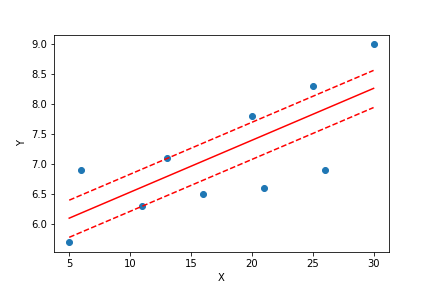
\includegraphics[width=0.5\linewidth]{figures/svr}
  \caption{Visualization of SVM classification.}
  \label{fig:svm}
\end{figure}

Equation \ref{eq-svm-1} defines the hyperplane, and Equation \ref{eq-svm-2} defines the hyperplanes of the support vectors, where $\phi(x)$ is the transformation from feature to kernel space that allows for non-linear solutions.
The margin between hyperplanes is equal to $1/||w||$, and then maximizing the margin is equivalent to minimizing $||w||$.
The optimization problem is solved by minimizing $J(w)$ in Equation \ref{eq-svm-3}:
\begin{align}
&w \cdot \phi(x_i) + b = 0    \label{eq-svm-1} \\
&w \cdot \phi(x_i) + b = \pm1 \label{eq-svm-2} \\
J(w) &= \frac{1}{2} ||w||^2 + C \sum_i \xi_i \label{eq-svm-3} \\
\intertext{such that}
y_i(&w \cdot \phi(x_i) + b) \geq 1-\xi_i \\
& \xi_i \geq 0
\end{align}
where $C$ is the regularization factor, which gives more weight to minimizing the flatness or the error, $\xi_i$ is the slack variable, which guards against outliers.
Some problems are not perfectly separable with a hyperplane.
The optimization of Equation \ref{eq-svm-3} allows some samples to be at a $\xi_i$ distance from their correct boundary.
A larger regularization parameter penalizes the approximation error, leading to its decrease during the optimization.
% An increase in the regularization parameter leads to a decrease of the approximation error.
% A larger $\epsilon$ decreases the number of support vectors, reducing the accuracy of the approximation.


\subsection{Decision Tree}

% steorts_tree_2017-1
% https://scikit-learn.org/stable/modules/tree.html#mathematical-formulation

The algorithm divides the predictor space into simple regions.
The set of splitting rules segmenting the predictor space can be visualized as an inverted tree, as shown in Figure \ref{fig:dt}.
Its branches connect internal nodes where a test determines in which sub-branch to continue.
The end of the tree contains the leaf nodes which make the final predictions.
The leaf nodes assign the most commonly occurring class of the training observations to new observations falling into those regions.

\begin{figure}[htbp!] %htbp! or H
  \centering
  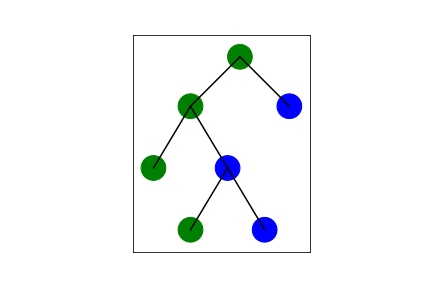
\includegraphics[width=0.5\linewidth]{figures/dt}
  \caption{Visualization of a decision tree.}
  \label{fig:dt}
\end{figure}

\Gls*{DT} uses a recursive binary split to grow the tree by minimizing an impurity function, which in this case is the Gini index \cite{pedregosa_scikit-learn_2011}, defined as
\begin{align}
& G = \sum_k p_{mk}(1-p_{mk}) \label{eq-dt}
\end{align}
where $p_{mk}$ is the proportion of class $k$ observations in the region node $m$.
A low Gini index indicates that a node contains predominantly observations from a single class.
Other measures of impurity include entropy and misclassification.
The package \textit{scikit-learn} uses the Gini index by default.

%The advantages of \glspl{DT} are that they are easy to interpret and that require little data preparation.
%Their main disadvantage is that complex trees are prone to overfitting.
%Predictions of decision trees are not continuous, but piecewise constant approximations.
%Therefore, they are not good at extrapolation.

% DTR
The algorithm for \gls*{DTR} is slightly different.
The tree can be visualized as a piecewise constant approximation.
For every new observation falling into the same space subregion, the leaf nodes assign the same prediction value, which is the average value of the training observations.
The training algorithm minimizes the \gls*{MSE} \cite{pedregosa_scikit-learn_2011}
\begin{align}
& MSE = \frac{1}{n_m} \sum_{y \in Q_m} \left( y - \bar{y}_m \right)^2 \label{eq-dtr} \\
& \bar{y}_m = \frac{1}{n_m} \sum_{y \in Q_m} y
\end{align}
where $\bar{y}_m$ is the learned mean value of the node.
$Q_m$ represents the data at node $m$ with $n_m$ samples.


\subsection{Random Forest}

% pedregosa_scikit-learn_2011

This method improves the performance of a single tree, as individual DTs may exhibit high variance.
This method reduces the overfitting and increases its precision.
The algorithm consists of a collection of decision trees.
It is based on the bootstrap aggregating method or \textit{bagging} \cite{breiman_bagging_1996}, which chooses the training data for each decision tree at random with replacement, fits the \glspl*{DT}, and then combines their results by voting.
The purpose of the randomness is to decrease the variance of the forest and decouple the prediction error \cite{pedregosa_scikit-learn_2011}.
% RFR
The algorithm for \gls*{RFR} is very similar, but instead of combining the different DT results by voting, the result is an average of the predictions of the different trees.


\subsection{K-Nearest Neighbors}

% https://scikit-learn.org/stable/modules/neighbors.html#classification

Neighbors-based classification does not create a model, but instead it stores instances of the training data \cite{pedregosa_scikit-learn_2011}.
Then, the algorithm classifies new samples based on the stored instances.
The KNNs are the $K$ training observations closest in distance to a new observation.
The Euclidean distance is the most common choice for measuring the distance between observations.
When classifying a new observation, the method assigns the data class which has the most representatives within the nearest neighbors of the point.
\gls*{KNN} is often successful in classification situations where the decision boundary is very irregular.

Figure \ref{fig:knn} displays an example of KNN classification, where the green dot is the sample to classify.
For a K value equal to three, the method uses the three closest samples to the green dot.
Two values are blue, and one is orange.
As the majority of the samples is blue, the method assigns the blue category to the new sample.

\begin{figure}[htbp!] %htbp! or H
  \centering
  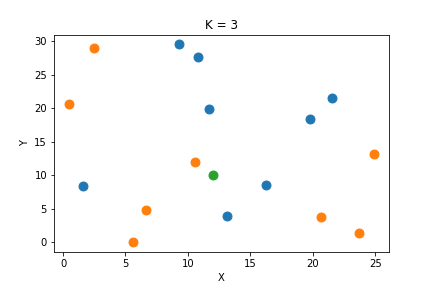
\includegraphics[width=0.5\linewidth]{figures/knns}
  \caption{Visualization of KNN classification.}
  \label{fig:knn}
\end{figure}

\subsection{Logistic Regression}

% https://scikit-learn.org/stable/modules/linear_model.html#logistic-regression

This type of regression determines the relationship between a binary dependent variable and a set of independent variables.
The method utilizes the sigmoid function, shown in Equation \ref{eq:logR-1}, to determine the likelihood of an observation to fall within each category.
The method determines the coefficients of the sigmoid function by minimizing a certain cost function.
This work uses the default setting of \textit{scikit-learn} which is to minimize the $L_2$-penalized cost function $J(w)$
% What loss? also, L2 regularization
\begin{align}
& \sigma(x_i) = \frac{1}{1+e^{-(w \cdot x_i + b)}} \label{eq:logR-1} \\
& J(w) = \frac{1}{2} ||w||^2 + C \sum_i log(exp(-y_i(w \cdot x_i + b))+1) \label{eq:logR-2}
\end{align}
where $C$ is the regularization factor.
% Like in support vector machines, smaller values specify stronger regularization.
Like in SVM, a larger regularization factor decreases the approximation error during the optimization.

Figure \ref{fig:logR} displays an example of logistic regression.
Most of the orange samples are located in the lower range of the independent variable $X$ while the blue samples are located in the upper range.
Then, training the model will assign values to the sigmoid function coefficients such that for new samples in the lower range of $X$, it will predict the $0$ category, while for new samples in the upper range of $X$, it will predict the $1$ category.

\begin{figure}[htbp!] %htbp! or H
  \centering
  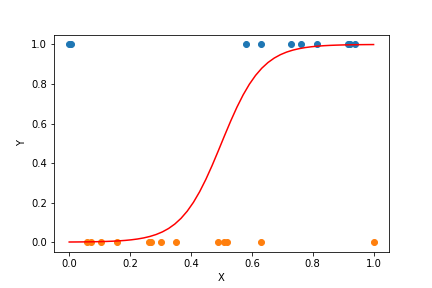
\includegraphics[width=0.5\linewidth]{figures/LogR}
  \caption{Visualization of logistic regression classification.}
  \label{fig:logR}
\end{figure}


\subsection{Feed-forward Neural Networks}

\Glspl*{FNN} are deep-learning architectures that learn complex relationships between inputs and outputs by mimicking biological networks of neurons.
A network consists of an input and output layer, and $M$ hidden layers of neurons, as shown in Figure \ref{fig:3-fnn}.

\begin{figure}[htbp!] % or H
  \centering
  \begin{subfigure}[b]{0.51\textwidth}
    \centering
    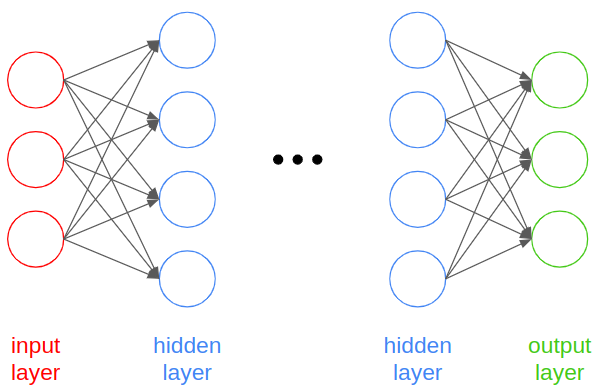
\includegraphics[width=1.0\textwidth]{figures/fnn-1}
    \caption{}
  \end{subfigure}
  \hfill
  \begin{subfigure}[b]{0.47\textwidth}
    \centering
    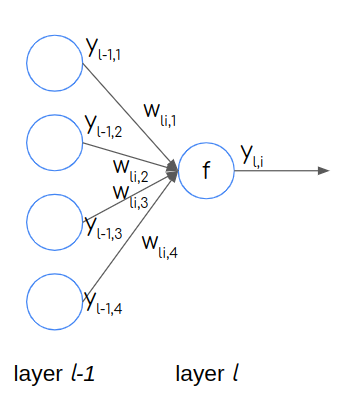
\includegraphics[width=0.65\textwidth]{figures/fnn-2}
    \caption{}
  \end{subfigure}
  \hfill
  \caption{Example of an FNN.}
  \label{fig:3-fnn}
\end{figure}

A neuron is connected to the neurons of the previous layer by weights.
Each neuron adds together the product of the neuron values in the previous layer and the weights connecting them plus a bias.
This summation serves as input to the next layer after applying an activation function, as stated in the following equation
\begin{align}
& y_{l, i} = f(w_{l, i}^T y_{l-1} + b_{l, i}) \label{eq-fnn-1} \\
& H = -\frac{1}{N} \sum_i y_i log(p(y_i)) + (1 - y_i) log(1 - p(y_i)) \label{eq-fnn-2}
\end{align}
where $y_{l, i}$ is the output of the node $i$ in layer $l$, $y_{l-1}$ output values of layer $l$-$1$, $f$ the activation function, and $w_{l, i}$ and $b_{l, i}$ the weights and biases connecting layer $l$-$1$ to the node $i$ of layer $l$.

Training the network sets the values of the connecting weights and biases by minimizing an error metric.
For the classification problem, the error metric is the binary cross-entropy, shown in Equation \ref{eq-fnn-2}, where $y_i$ is the label, $p(y_i)$ is the predicted probability of the point to be \textit{true}, and $N$ is the number of samples.

% FNNs for regression
When using the FNN for regression, the algorithm trains the network by minimizing the MSE
\begin{align}
MSE = \frac{1}{N} \sum_i (Y_i - \hat{Y_i})^2 \label{eq-MSE}
\end{align}
where $\hat{Y_i}$ is the predicted output of the node $i$ of the output layer of the network, $Y_i$ is the target value, and $N$ is the number of nodes in the output layer times the number of samples.


\subsection{Long-Short Term Memory Networks}
\label{sec:lstm}

% LSTMs
% https://colah.github.io/posts/2015-08-Understanding-LSTMs/
% https://www.analyticsvidhya.com/blog/2021/03/introduction-to-long-short-term-memory-lstm/
Although RNNs are neural networks that handle inputs and outputs correlated as part of a sequence, they cannot learn long-term dependencies.
When training the network, the back-propagated gradients may grow or shrink significantly at each time step.
Therefore, the gradients may vanish or explode for time series with long duration.
LSTMs are a special kind of RNN that were explicitly designed to avoid the vanishing gradient problem and are able to learn long-term dependencies.

% LSTM - Structure
The LSTM cell consists of three parts, better known as gates: the forget gate, the input gate, and the output gate, shown in Figure \ref{fig:lstm}.
The forget gate determines if the information from the previous timestamp is forgotten, the input gate controls the flow of new information, and the output gate updates the information into the next timestamp.
The gates allow the LSTM to add or remove information to the cell state $C_t$ and hidden state $h_t$.
The cell and hidden states are also known as long-term and short-term memory, respectively.

\begin{figure}[htbp!] %htbp! or H
  \centering
  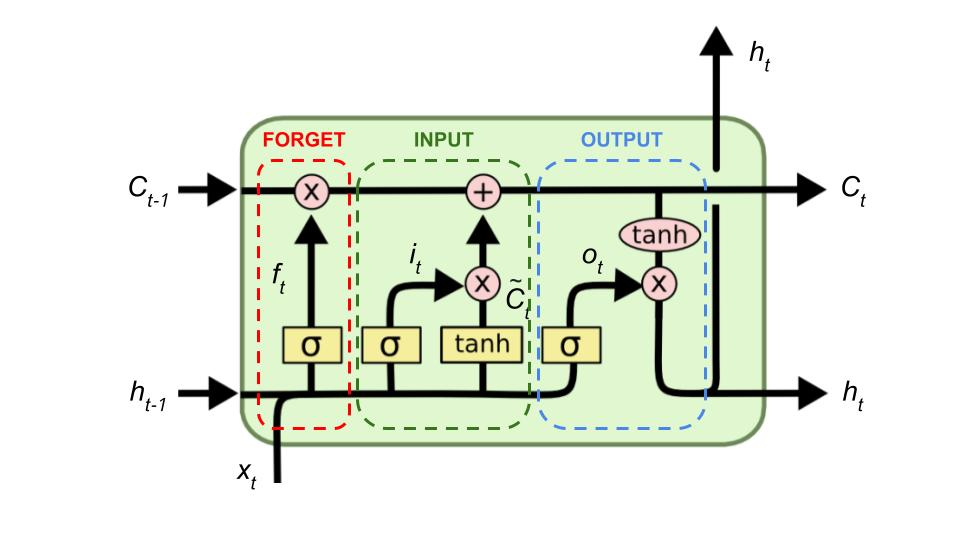
\includegraphics[width=0.5\linewidth]{figures/lstm}
  \caption{LSTM structure.}
  \label{fig:lstm}
\end{figure}

% Equations
The following sets of equations are the mathematical definition of the LSTM cell
\begin{align}
f_t &= \sigma \left( W_f h_{t-1} + U_f x_t + b_f \right)  \label{eq:lstm1} \\
i_t &= \sigma \left( W_i h_{t-1} + U_i x_t + b_i \right)  \label{eq:lstm2} \\
\tilde{C}_t &= tanh \left( W_C h_{t-1} + U_C x_t + b_C \right)  \label{eq:lstm3} \\
C_t &= f_t \cdot C_{t-1} + i_t \cdot \tilde{C}_t          \label{eq:lstm3} \\
o_t &= \sigma \left( W_o h_{t-1} + U_o x_t + b_o \right)  \label{eq:lstm4} \\
h_t &= o_t \cdot tanh \left( C_t \right)                  \label{eq:lstm5}
\end{align}
where $W$ and $b$ are the weights and biases for the different layers as in any other type of network.
The forget gate output $f_t$ is a number between 0 and 1, wherein a value of 0 means forget everything, and a value of 1, forget nothing.
In the input gate, $i_t$ defines which values to update, and $\tilde{C}_t$ comprises the candidate values that can be added into the cell state.
The cell state $C_t$ is calculated as the addition of the values not forgotten from the previous cell state $C_{t-1}$ and the new updated values $\tilde{C}_t$.
Finally, the hidden state $h_t$ is a filtered version of the cell state $C_t$, and $o_t$ decides what information is included.
% This technique is able to consider additional explanatory variables while learning across time-series \cite{calkoen_traditional_2021}.

Overall, the network can be visualized as a mathematical function whose inputs are the time-dependent features $x_t$ which produce the time-dependent outputs $h_t$.
The training of the network is a bit more cumbersome than for other neural networks.
As both the features and outputs are time-dependent, the common training strategy converts the time-dependent problem into a static supervised problem, wherein the output of previous time steps act as input to the next time step.
The supervised problem separates the data into \textit{look-back} and \textit{look-forward} steps.
The look-back steps are the number of steps that the network uses to predict a certain number of look-forward steps at a time.
Figure \ref{fig:lstm-convert} displays an example of the conversion process.
For the output time-series $h$, with $N_t$ time steps, the input and output of the supervised problem take the shape $(N_t-N_{lb}-N_{lf}) \times N_{lb}$ and $(N_t-N_{lb}-N_{lf}) \times N_{lf}$, respectively, where $N_{lb}$ and $N_{lf}$ are the number of look-back and look-forward steps.
Additionally, the network is able to learn a dependency on the features $x_t$ by adding this information to the inputs of the supervised problem.
Assuming static features $x_t = x$, the input of the supervised problem takes the shape $(N_t-N_{lb}-N_{lf}) \times (N_x + N_{lb})$, where $N_x$ is the number of features.

% Conversion from unsupervised to supervised problem
% y_test = [N_samples x (len_t_series-lookback-lookforward) x lookforward]
% N = N_samples x (len_t_series-lookback-lookforward) x lookforward
\begin{figure}[htbp!] %or H 
  \centering
  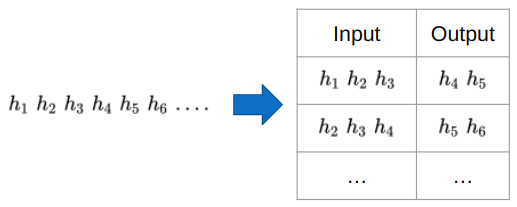
\includegraphics[width=0.50\linewidth]{figures/lstm_convert}
  \hfill
  \caption{Example of conversion of a time-series into a supervised problem.}
  \label{fig:lstm-convert}
\end{figure}

Finally, training the network sets the values of the connecting weights and biases by minimizing an error metric.
This work uses the \gls*{MAE}
\begin{align}
MAE = \frac{1}{N_{samples} \times (N_t-N_{lb}-N_{lf}) \times N_{lf}} \sum_i | Y_i - \hat{Y_i} | \label{eq-MAE}
\end{align}
where $\hat{Y_i}$ is predicted output, $Y_i$ is the output of the supervised problem or target value, and $N_{samples}$ is the number of samples.


\subsection{Optimization}
\label{sec:opt}

% https://distill.pub/2020/bayesian-optimization/
% https://mlconf.com/blog/lets-talk-bayesian-optimization/

Some of the machine learning algorithms described above allow the user to specify their hyperparameter values to improve the results.
To obtain the best result, this work uses Bayesian optimization for the hyperparameter tuning.

% BAYESIAN OPTIMIZATION USING GAUSSIAN PROCESSES
Bayesian optimization targets systems where the objective function $f$ does not have a closed form or is expensive to evaluate.
The idea of Bayesian methods is to update the current hypothesis as new information becomes available.
The process initialization uses a Gaussian process as a prior probability distribution.
In Gaussian processes, every finite collection of random variables has a multivariate normal distribution.

The prior probability represents what is originally believed before new evidence is introduced.
The routine updates a posterior probability distribution of $f$ every time a new function evaluation is reported.
This posterior model is a simpler surrogate function $\hat{f}$ approximating the objective function. 

The surrogate is easier to optimize than the objective function.
The method finds the sample that performs best on the surrogate function to evaluate it on the objective function.
An acquisition function guides the selection of the next sample from the search space.
The \textit{expected improvement} is one of the most common acquisition functions, and it indicates the region of the search space that is most likely to improve.
Overall, this method reduces the number of evaluations necessary to determine the optimal parameters.

In summary, the algorithm can be itemized as follows
\begin{enumerate}
\item Place a Gaussian process prior on $f$.
\item Observe $f$ for random samples of the search space.
\item Update the $\hat{f}$ using all the available data.
\item Find the point in the search space $x_i$ that maximizes the acquisition function.
\item Get a new observation of $f$ at $x_i$.
\item Repeat 3- to 5- until convergence.
\end{enumerate}

\begin{figure}[htbp!] % or H
  \centering
  \begin{subfigure}[b]{0.49\textwidth}
    \centering
    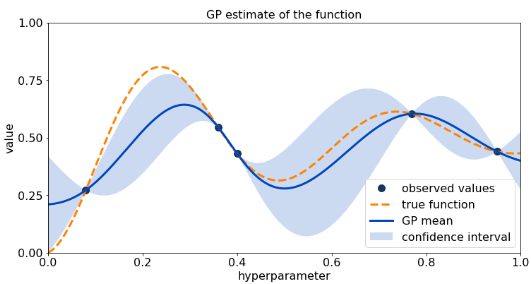
\includegraphics[width=0.85\textwidth]{figures/BO-GP-1}
    \caption{}
  \end{subfigure}
  \hfill
  \begin{subfigure}[b]{0.49\textwidth}
    \centering
    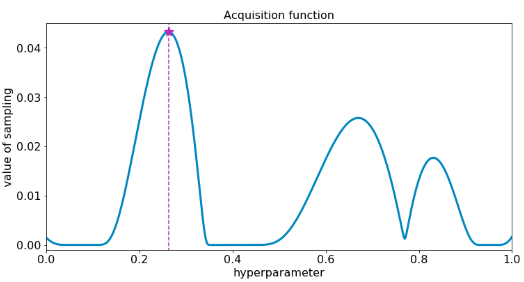
\includegraphics[width=0.85\textwidth]{figures/BO-GP-2}
    \caption{}
  \end{subfigure}
  \par
  \begin{subfigure}[b]{0.49\textwidth}
    \centering
    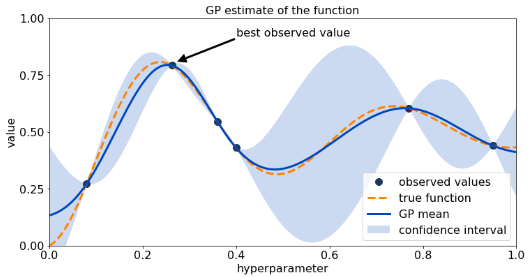
\includegraphics[width=0.85\textwidth]{figures/BO-GP-3}
    \caption{}
  \end{subfigure}
  \caption{Example of Bayesian Optimization process. Image reproduced from \cite{ravikumar_lets_2018}.}
  \label{fig:3-bo}
\end{figure}

Figure \ref{fig:3-bo} displays items 3- to 5-, where $\hat{f}$ is updated with all the available data, the process finds the point $x_i$ that maximizes the acquisition function, and finally, $f$ is evaluated at the new observation point $x_i$. 
This work utilizes Bayesian optimization using Gaussian processes implemented through the \textit{gp\_minimize} function \cite{scikit_optimize} to optimize the different machine learning algorithms.


\section{Simplified Model}
\label{sec:simpl-model}

% Intro
This section introduces a simplified physics-based model to investigate the feasibility of training and testing a data-based model that can capture the physics of the problem.
% Model description
The model represents a post-irradiation experiment that is cooled by the natural circulation of air, and it comprises a conjugate heat transfer problem characterized by a cavity filled with air and a multi-region solid, as shown in Figure \ref{fig:tf-geo}.
The solid consists of an experiment embedded in a capsule.
To decrease the computational burden, the model is reduced to a two-dimensional problem.
This model neglects the heat production ($q''' = 0$) in the capsule to simplify the analysis.
This assumption is justified by the fact that the volume of the experiment is considerably larger than the capsule's.
% This is a conservative assumption.
% In the three-dimensional problem, the experimental device has a larger surface-area-to-volume ratio, and therefore, a higher heat loss rate and lower temperatures.
% BC and ICs
The boundary conditions defining the problem are adiabatic walls on the side and top edges, while the temperature at the bottom of the geometry is fixed at room temperature (298 K or 25 $^\circ$C), as shown in Figure \ref{fig:tf-geo}.
The initial condition is room temperature for the whole geometry.

\begin{figure}[htbp!] %or H 
    \centering
    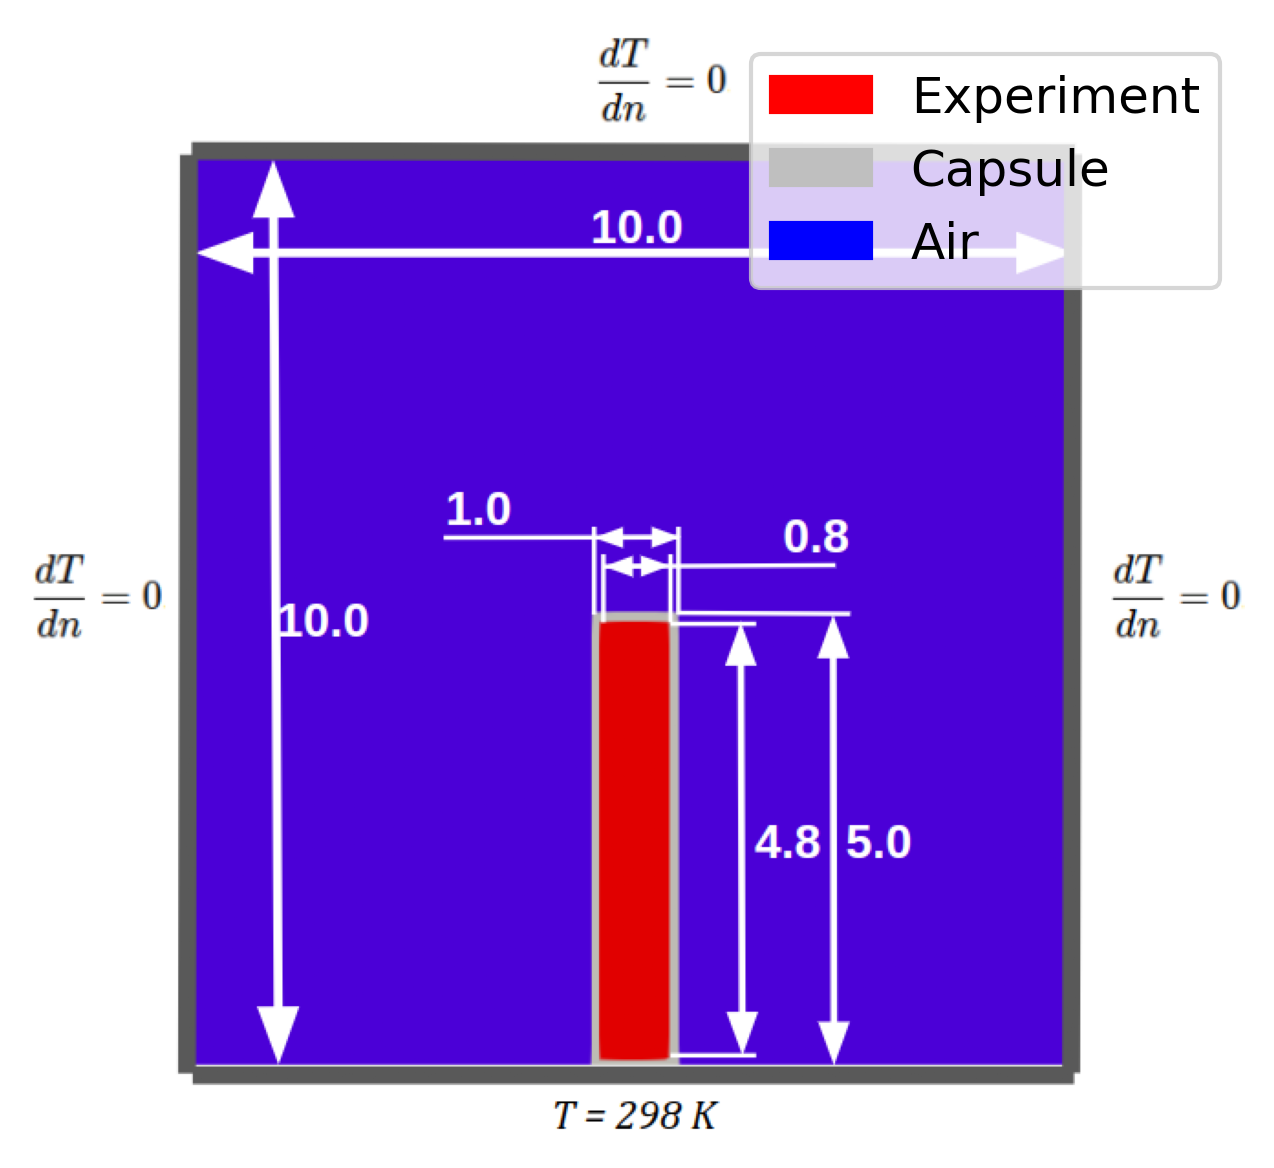
\includegraphics[width=0.5\linewidth]{figures/tf-geo-simple2}
    \hfill
    \caption{Two-dimensional geometry of a post-irradiation experiment cooled by the natural circulation of air. All dimensions are expressed in $cm$.}
    \label{fig:tf-geo}
\end{figure}

% Laminar flow
This model assumes a laminar flow for solving the equations of motion and temperature of the air.
The following correlation defines the transition to the turbulence regime for a vertical plate in natural circulation \cite{incropera_fundamentals_2006}
\begin{equation}
Ra_{x,c} = \frac{g \beta \Delta T x^3}{\nu \alpha} \approx 10^9,
\end{equation}
where $Ra_{x,c}$ is the critical Rayleigh number at $x$ distance from the bottom, $g$ is the acceleration due to gravity, $\beta$ is the thermal expansion coefficient, $\Delta T$ is the difference between the surface temperature and the air reference temperature, $\nu$ is the kinematic viscosity of the air, and $\alpha$ is the thermal diffusivity of the air.
For these simulations, the Rayleigh number is well below 10$^9$.


\subsection{Model verification}

This exercise uses MOOSE to solve the physics-based model and OpenFOAM to verify it.
% fairhurst-agosta_machine_2022 & fairhurst-agosta_machine_2_2022 
As mentioned earlier, MOOSE relies on the Boussinesq approximation for solving the equations of motion and temperature of the air.
This approximation may be inaccurate for large gradients of temperature in the fluid.
For this reason, this section compares the results from MOOSE and OpenFOAM, which solves the motion and temperature of the air as well as its density without approximation.
Additionally, even though the Boussinesq approximation may yield an inaccurate fluid temperature, the comparison metric is the time evolution of the highest temperature in the capsule.
MOOSE and OpenFOAM determine the point in the capsule's geometry with the highest temperature, and this work refers to it as the highest temperature in the capsule.

% the exercise
% material properties
Table \ref{tab:tf-mat} specifies the material properties of the different regions included in the model.
For simplicity, both the capsule and the experiment are made of iron.
Note that the properties of the fluid for the thermal-fluid solvers differ, as MOOSE solves the Boussinesq equations while OpenFOAM solves for the density.
% source details
The experiment heat source decays with respect to time with the shape of 1.25 $\times$ 10$^9$ W/m$^3$ $e^{-t}$ whose initial value is equivalent to 10 kW.

\begin{table}[htbp!]
  \centering
  \caption{Material properties of the thermal-fluids model.}
  \label{tab:tf-mat}
  \begin{tabular}{cccccc}
    \toprule
      Properties & Units    & Capsule              & Experiment            & Air MOOSE                & Air OpenFOAM \\
    \midrule
      $\rho$     & kg/m$^3$ & 8 $\times$ 10$^{3}$  & 2.7 $\times$ 10$^{3}$ & 1.2                      & - \\
      $k$        & W/m/K    & 80                   & 80                    & 2.6 $\times$ 10$^{-2}$   & - \\
      $c_p$      & J/kg/K   & 450                  & 450                   & 1000                     & 1000 \\
      $\mu$      & kg/m/s   & -                    & -                     & 1.8 $\times$ 10$^{-5}$   & 1.8 $\times$ 10$^{-5}$ \\
      Pr         & -        & -                    & -                     & -                        & 0.7 \\
      $\beta$    & 1/K      & -                    & -                     & 3.356 $\times$ 10$^{-3}$ & - \\
    \bottomrule
  \end{tabular}
\end{table}

% Results
Figure \ref{fig:tf-val} shows the time evolution of the highest temperature in the capsule calculated by MOOSE and OpenFOAM.
The temperature in the capsule increases sharply from the initial condition of 298 K.
The maximum temperature is 562 K and is reached at 4.2 s of the simulation start.
Both MOOSE and OpenFOAM predict an almost identical time evolution, demonstrating that MOOSE predicts an accurate temperature evolution.

\begin{figure}[htbp!] %or H 
    \centering
    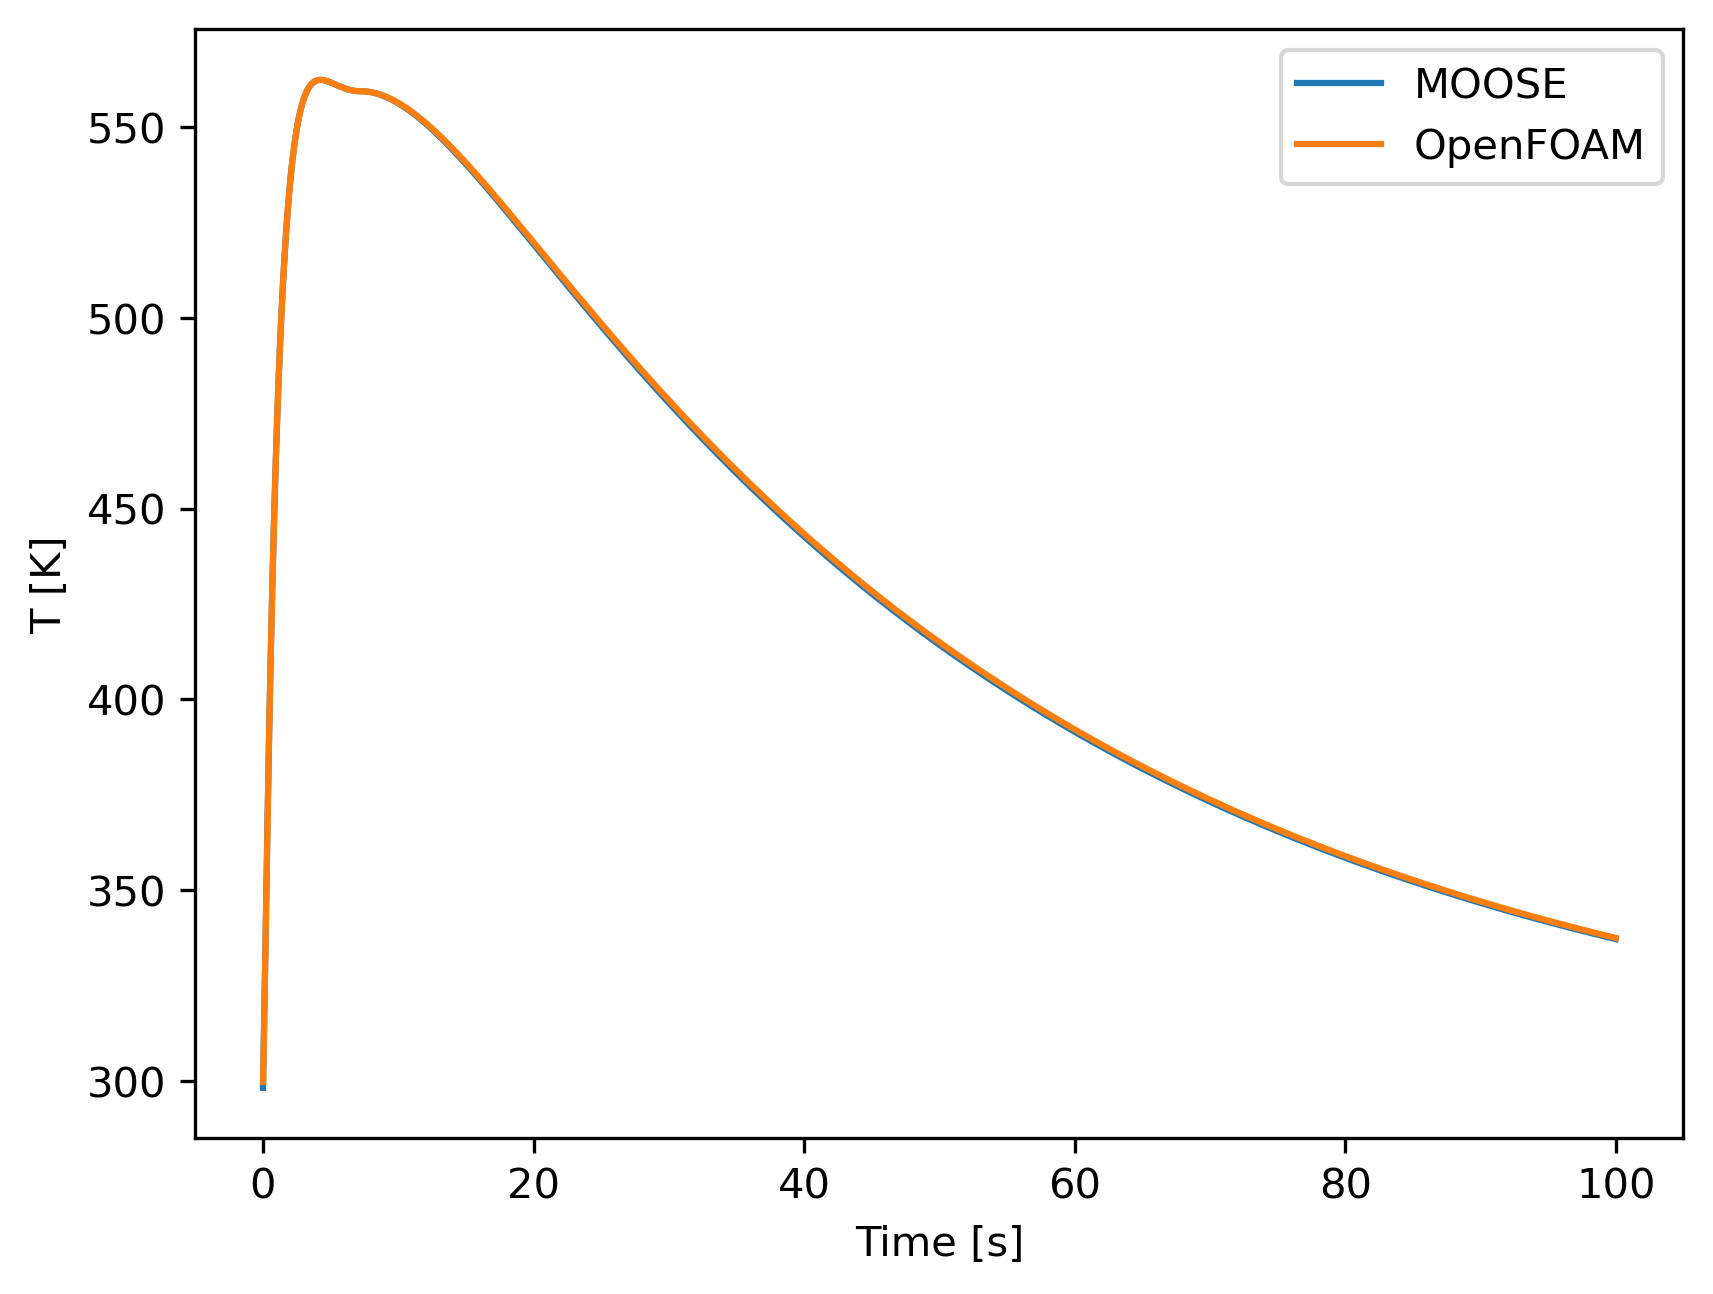
\includegraphics[width=0.45\linewidth]{figures/verification}
    \hfill
    \caption{Time evolution of the highest temperature in the capsule calculated by MOOSE and OpenFOAM.}
    \label{fig:tf-val}
\end{figure}

Figure \ref{fig:tf-tfin} displays the temperature distribution in the experiment and the capsule when the capsule reaches the peak temperature.
The highest temperature in the capsule is located in the half top, at 1.85 cm from the top.
% The original expectation was to find the highest temperature on top of the experiment.
% However, the heat released in the radial direction is greater than in the axial direction, due to the geometries of the experiment and the capsule.
In the radial direction, and as expected, the highest temperature is located on the inner wall, where the capsule wall meets the experiment.
As the experiment produces heat, it is natural to consider that its temperature will be above the capsule temperature.
Hence, the highest temperature in the capsule is in the region closest to the experiment.

\begin{figure}[htbp!] %or H 
    \centering
    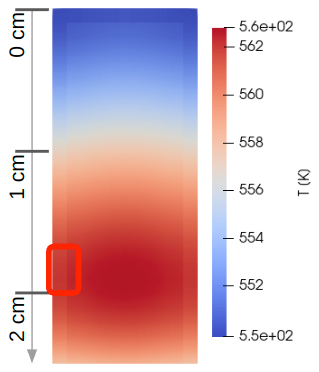
\includegraphics[width=0.27\linewidth]{figures/T_tmax}
    \hfill
    \caption{Temperature distribution in the experiment and capsule when the capsule reaches the peak temperature. The red square highlights the location of the highest temperature in the capsule.}
    \label{fig:tf-tfin}
\end{figure}

% Conclusions
% Let's add more figures and draw conclusions from them, like we shouldn't have an adiabatic BC on the top.
The model used in this exercise is generic and reactor-agnostic, meaning that it can be tailored to any research reactor.
Additionally, this exercise considers an adiabatic boundary condition on the top of the geometry, which does not allow for heat removal or fluid flow in case of a real accident.
The final dimensions and boundary conditions of the model are specific to each experiment/reactor configuration and should be tailored accordingly.
% radiation and turbulence
Moreover, the large temperature shown in the results highlights that radiation heat transfer needs to be included in the model to obtain a more accurate representation of the experiments.
Furthermore, the turbulence regime is highly dependent upon the geometry of the experiment, which is specific to the reactor under study.
Hence, the assessment of the turbulence regime for each specific geometry is necessary.
Although this model has certain limitations, this exercise intends to simplify the creation and understanding of a data-based model as well as drawing some useful conclusions.


\subsection{Data Processing and Model Training}
\label{sec:datapros}

Machine learning derives relationships from data, allowing data-based models to solve complex problems quickly.
In this exercise, the collected data comprises the time evolution of the highest temperature in the capsule for certain material properties: density $\rho$, thermal conductivity $k$, and heat capacity $c_p$; and the coefficients defining the delayed heating: initial value $q0$ and decay time $\tau$.
These five coefficients are the input variables or \textit{features} of the model, and the highest temperature in the capsule is the output or \textit{label}.
The thermal properties values correspond to the 33 first materials that are shown in Appendix \ref{ap:mat_props}, including all materials from aluminum to iridium.
$q_0$ comprises 45 uniformly distributed values between 10$^7$ and 10$^8$ W/m$^3$, and 20 between 10$^8$ and 5 $\times$ 10$^8$ W/m$^3$, totaling 65 unique values.
$\tau$ comprises five uniformly distributed values between 20 and 100 seconds.
The combination of all these variables leads to a total of 10725 samples.

The simulation time of the physics-based model was 500 seconds, recording the time evolution in 51 non-uniformly distributed time steps.
In summary, the data constitute the input variable $X$ and the output variable $Y$, having shapes of $N_{samples} \times N_{features}$ and $N_{samples} \times N_{timesteps}$, respectively, with $N_{samples}$=10725, $N_{features}$=5, and $N_{timesteps}$=51.
Figure \ref{fig:tf-data1} provides a visual representation of the input/output pairs of the physics-based model.

\begin{figure}[htbp!] %or H 
    \centering
    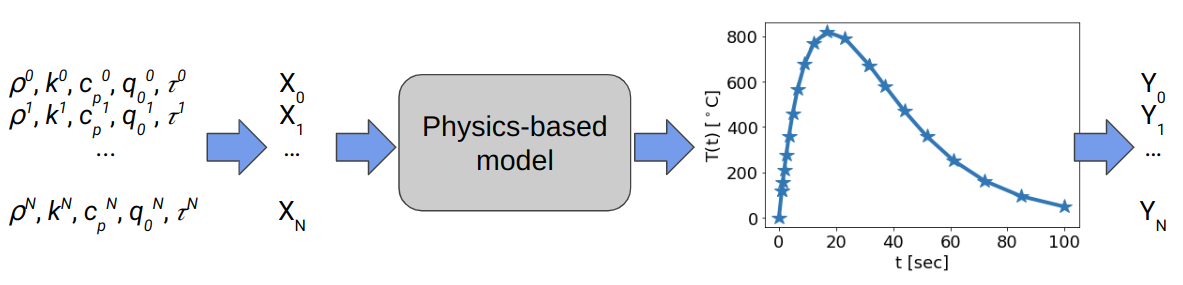
\includegraphics[width=0.85\linewidth]{figures/data-process}
    \hfill
    \caption{Physics-based model input/output pairs.}
    \label{fig:tf-data1}
\end{figure}

The prediction of the capsule state considered two different strategies.
The first strategy forecasts only whether the capsule melts or not.
This is a binary classification problem, in which the two possible outcomes are \textit{melt} and \textit{does not melt}.
The second strategy solves a time-evolution prediction problem, which determines if the capsule melts as well as the time of occurrence.
The time of occurrence can better guide the operators’ countermeasures in case of an accident.
% Such a study could guide operators' preventive actions in the event of an accident.
When the melting time is a required feature of the model, the data-based model has to forecast the entire time evolution of the highest temperature in the capsule.
Once the model predicts the time evolution, it becomes straightforward to resolve if the capsule melts and determine the melting time.

% Performance metrics
The chosen performance metrics are the accuracy, recall, and training time for the classification problems, and the accuracy, recall, mean melting-time relative error, and maximum melting-time relative error for the time-evolution prediction problem.
The accuracy and recall are calculated as follows
\begin{align}
Accuracy &= \frac{TN + TP}{TN + FN + TP + FP} \\
Recall &= \frac{TP}{TP + FN}
\end{align}
where $TN$ is the number of true negative results, $TP$ is the number of true positive results, $FN$ is the number of false negative results, and $FP$ is the number of false positive results.

The accuracy is the ratio of the correctly classified samples over the total number of samples.
The recall is the ratio between correctly classified relevant samples over the total number of relevant samples.
The accuracy does not provide information on the distribution of the correctly classified samples.
The recall resolves this issue, indicating the quality of the classification within each category.
This work uses the recall of the melting category, which is the ratio between the number of samples predicted to melt over the total number of samples that melt.
This approach is more conservative than using the recall of the non-melting category.
If the model predicts that a sample melts when it does not, any consequential corrective measure will not trigger a radioactive material release.
The confusion matrix, shown in Figure \ref{fig:conf-matrix}, aids in the visualization of the performance of classification algorithms.

\begin{figure}[htbp!] %htbp! or H
  \centering
  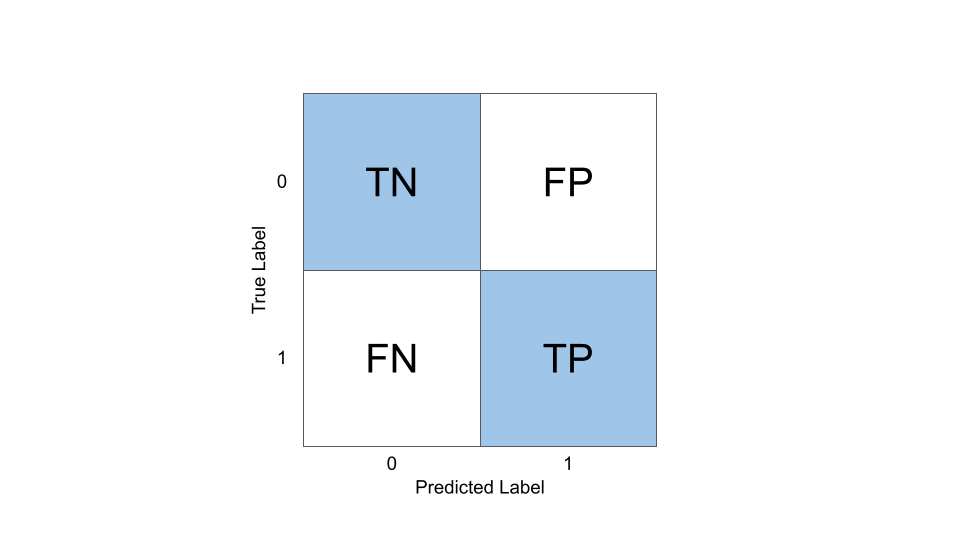
\includegraphics[width=0.7\linewidth]{figures/confusion_matrix}
  \caption{Confusion matrix. T: True, F: False, N: Negative, P: Positive.}
  \label{fig:conf-matrix}
\end{figure}

The data handling process for the classification problem is summarized in Figure \ref{fig:data-class}.
The output variable $Y$ is transformed into the binary variable $\bar{Y}$, in which $0$ represents that the capsule \textit{does not melt} and $1$ that it \textit{melts}.
If the temperature of a sample goes over the capsule melting temperature, then, $\bar{Y}$ takes the value 1, and 0 otherwise.
This work considers a capsule melting temperature of 923 K (650 $^{\circ}$C).

\begin{figure}[htbp!] %htbp! or H
  \centering
  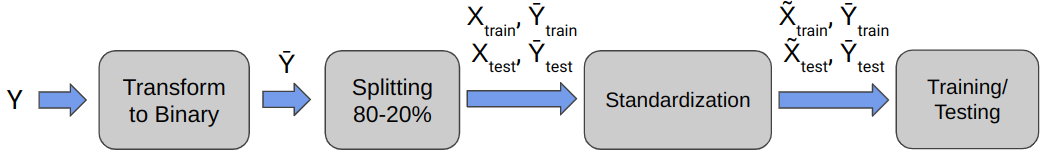
\includegraphics[width=0.7\linewidth]{figures/data-pross-classification}
  \caption{Classification problem data handling.}
  \label{fig:data-class}
\end{figure}

The pre-processing of the data involves the splitting and standardization.
The samples are randomly split into training and testing datasets.
Of the samples, 80\% integrate the training dataset, and the remaining 20\%, the testing dataset.
The standardization method scales the datasets by subtracting the mean value $\mu$ of the samples and dividing the result by the standard deviation $\sigma$ for each feature $j$

\begin{align}
\tilde{X}^j = (X^j - \mu^j) / \sigma^j.
\end{align}

Standardization is a feature scaling technique that is a common requirement for many machine learning estimators.
If a feature has a variance that is orders of magnitude larger than the others, it might dominate the objective function, falling within a local minimum during training and making the estimator unable to learn as expected.
After the data pre-processing, the data-based model is trained using the training dataset for the standardized input and output variables $\tilde{X}_{train}$ and $\bar{Y}_{train}$.
The data-based model uses the following machine learning techniques: DT, FNN, KNN, LogR, RF, and SVM.
Once the model is trained, the model can predict the outcome of the transient by reading the material properties of a specific sample and coefficients defining the delayed heating, as shown in Figure \ref{fig:data-class0}.

\begin{figure}[htbp!] %htbp! or H
  \centering
  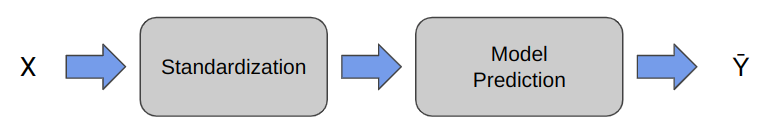
\includegraphics[width=0.7\linewidth]{figures/data-prediction}
  \caption{Visualization of classification prediction.}
  \label{fig:data-class0}
\end{figure}

The only optimized methods were the KNNs and the FNNs, while the rest of the methods utilized the \textit{scikit-learn} default parameters.
The optimization of the KNN was carried out via grid search and explored different numbers of N-nearest neighbors to maximize the recall.
The optimization of the FNN was based on Bayesian optimization using Gaussian Processes (Section \ref{sec:opt}) to maximize the recall.
The training of the network used the Adam optimizer to minimize binary cross-entropy.
The FNN number of layers was fixed to four, for which the input and output layers had five and one node, respectively, and the two hidden layers had a variable number of nodes.
The optimization of the FNN determined the number of nodes and training batch size.
The optimal configuration was 104 and 155 nodes for the hidden layers, and a batch size of 16.

% Strategy from fairhurst-agosta_machine_2_2022
Figure \ref{fig:data-class1} displays the prediction of the time-evolution prediction problem.
The output is the whole time evolution of the highest temperature in the capsule, which is translated into $\bar{Y}$ containing the \textit{melt}/\textit{does not melt} outcome as well as the capsule's melting time.
This work uses three different approaches to predict the time evolution, and the data handling process is slightly different for each of them.

\begin{figure}[htbp!] %htbp! or H
  \centering
  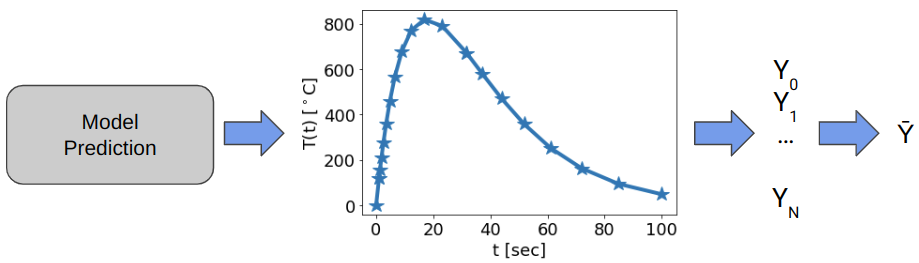
\includegraphics[width=0.7\linewidth]{figures/data-prediction-t}
  \caption{Visualization of time-evolution prediction.}
  \label{fig:data-class1}
\end{figure}

The first method is based on the regression of non-linear fitting coefficients defining the time evolution.
As a decaying exponential defines the heat production in the experimental device, it is natural to assume that the temporal behavior of the sample temperature is also a combination of decaying exponentials, and the curve $A (e^{-\lambda_1 t} - e^{-\lambda_2 t})$ approximates the temperature response well.
A non-linear curve fitting uses the \textit{curve\_fit} function \cite{2020SciPy-NMeth} to determine the coefficients of the curve $A$, $\lambda_1$, and $\lambda_2$.
Figure \ref{fig:nlin-fit} displays an example of the non-linear curve fitting to discretize the capsule temperature evolution.

\begin{figure}[htbp!] %htbp! or H
  \centering
  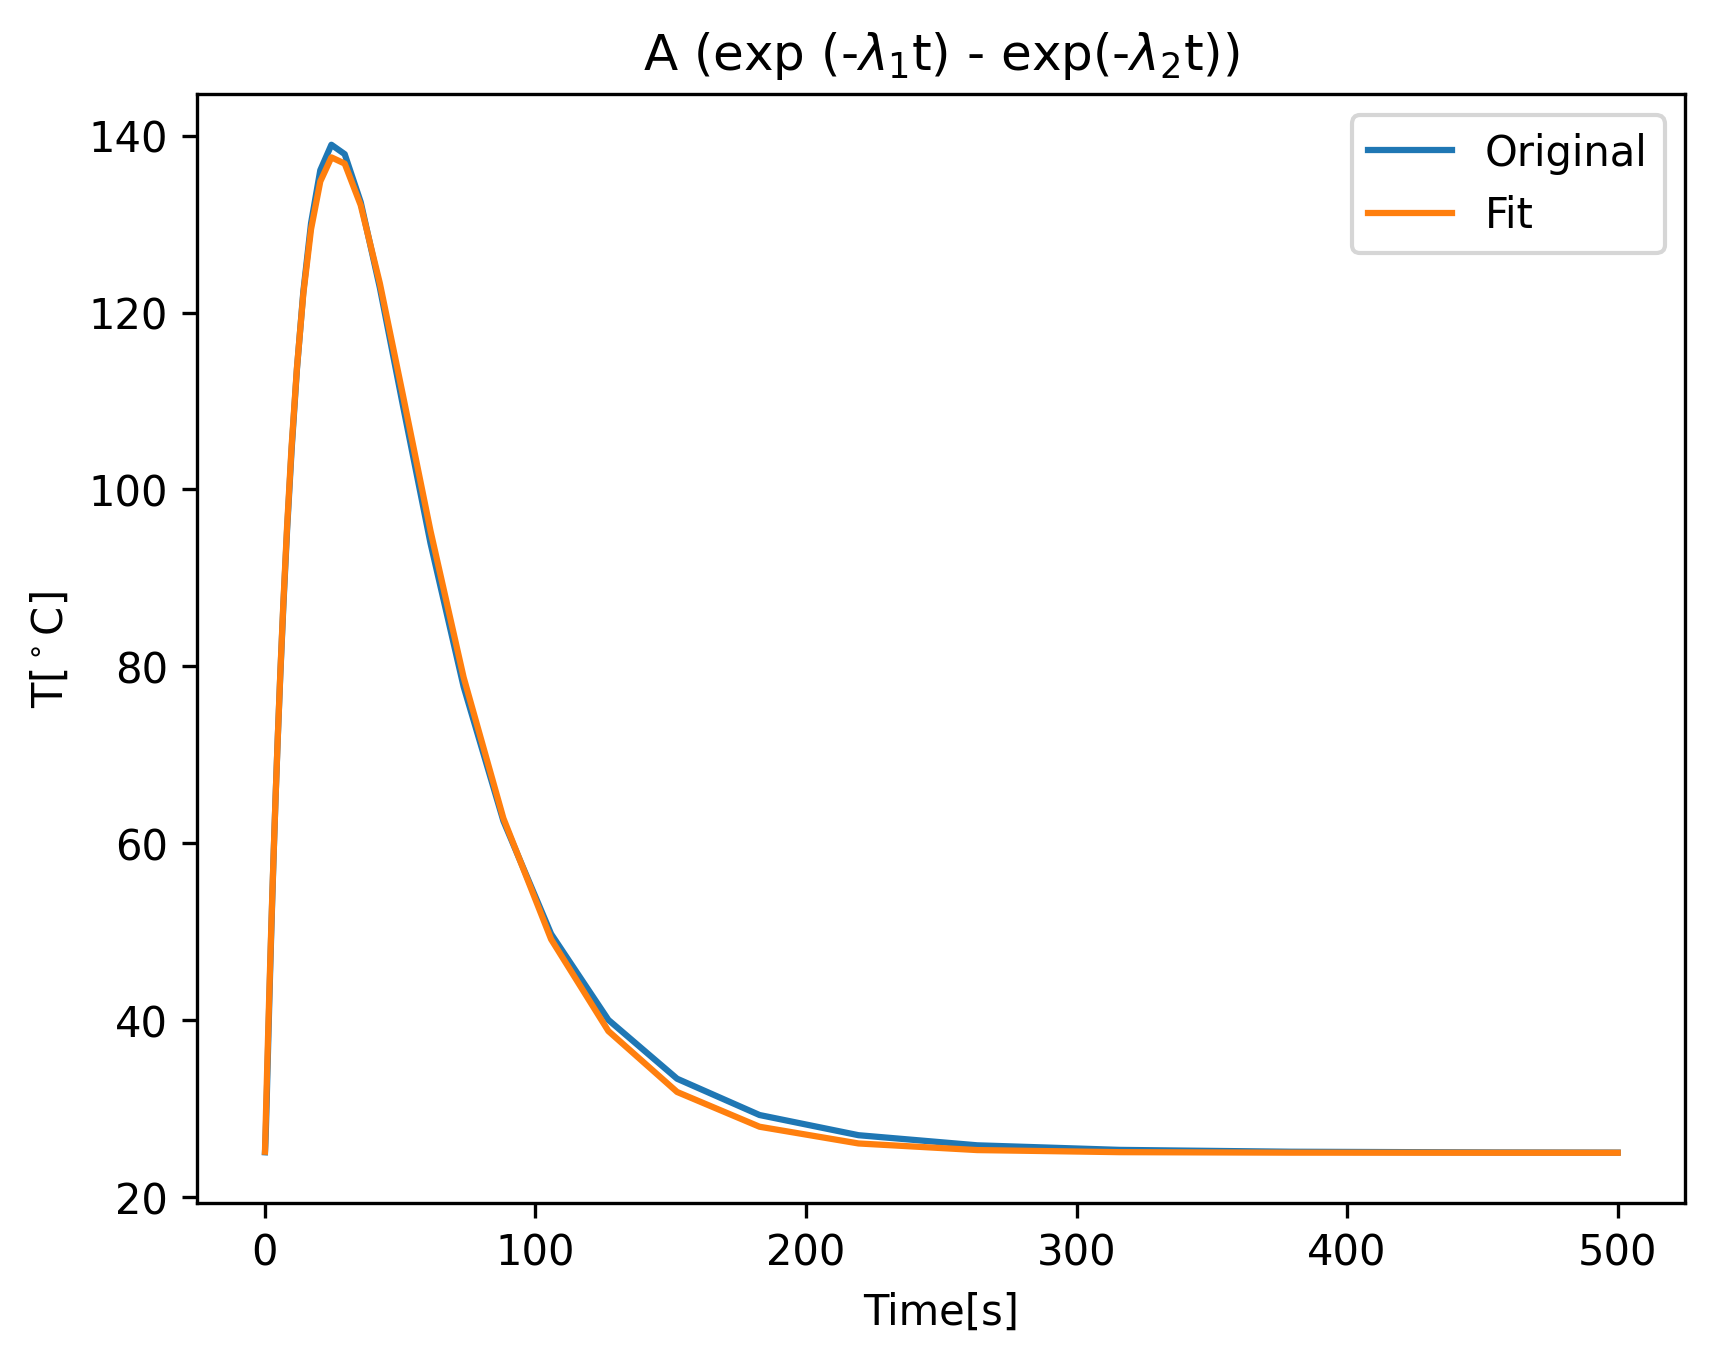
\includegraphics[width=0.50\linewidth]{figures/non-linear-fit}
  \caption{Example of the non-linear curve fitting to discretize the capsule temperature evolution.}
  \label{fig:nlin-fit}
\end{figure}

\begin{figure}[htbp!] %htbp! or H
  \centering
  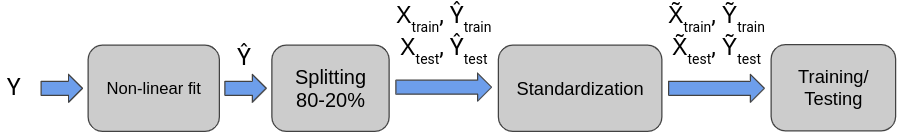
\includegraphics[width=0.7\linewidth]{figures/data-pross-regression}
  \caption{Data handling process for the time-evolution prediction using regression of non-linear fitting coefficients.}
  \label{fig:data-reg}
\end{figure}

The data handling process for this method is summarized in Figure \ref{fig:data-reg}.
The coefficients $A$, $\lambda_1$, and $\lambda_2$ compose an intermediate output variable $\hat{Y}$ with shape $N_{samples} \times 3$.
The samples are separated into an 80-20 training-testing split, and standardization is applied.
The data-based model is trained with the standardized input and output variables, $\tilde{X}_{train}$ and $\tilde{Y}_{train}$.
Once the model is trained, the model can predict the outcome of the transient by reading the material properties of a specific sample and coefficients defining the delayed heating, as shown in Figure \ref{fig:data-reg1}.
Then, the trained model predicts $\tilde{Y}$ that is used to reconstruct the temperature time evolution $Y$, and obtain the output variable $\bar{Y}$.
This work uses \gls*{LR}, \gls*{SVR}, \gls*{DTR}, and \gls*{RFR} to build the data-based model.
However, some of these methods are unable to capture the non-linear behavior of the different curve fitting coefficients.
Section \ref{sec:comp} discusses the results for the best-performing methods -- \gls*{DTR} and \gls*{RFR}.
These models were not optimized and used \textit{scikit-learn} default parameters to reduce the complexity.

\begin{figure}[htbp!] %htbp! or H
  \centering
  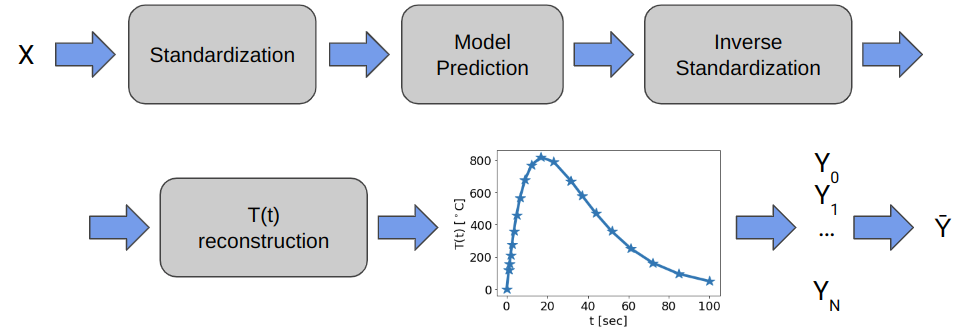
\includegraphics[width=0.7\linewidth]{figures/data-prediction-tEvol-nlf}
  \caption{Visualization of time-evolution prediction using regression of non-linear fitting coefficients.}
  \label{fig:data-reg1}
\end{figure}

% FNN MODEL
The second method uses FNNs to predict the whole time evolution of the highest temperature in the capsule at once.
The data handling process for this method is summarized in Figure \ref{fig:data-fnn}.
The samples are separated into an 80-20 training-testing split.
After splitting the data into training and testing datasets, the datasets are scaled.
The input variables $X_{train}$ and $X_{test}$ are standardized, while the output variables $Y_{train}$ and $Y_{test}$ are normalized instead.
Normalization is a feature scaling technique that uses the maximum and minimum value of each feature to scale the data
\begin{align}
\tilde{X}^j = (X^j - X_{min}^j) / (X_{max}^j - X_{min}^j).
\end{align}

\begin{figure}[htbp!] %htbp! or H
  \centering
  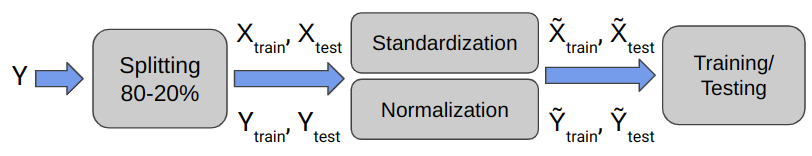
\includegraphics[width=0.7\linewidth]{figures/data-pross-fnn}
  \caption{Data handling process for the time-evolution prediction using FNNs.}
  \label{fig:data-fnn}
\end{figure}

% Formula
% What is the standard approach
The network training used the Adam optimizer to minimize the \gls*{MAE}.
The neural network had a 5-node input layer, two hidden layers, and a 51-node output layer.
The network optimization set the number of nodes in the hidden layers, the training learning rate, and training batch size.
% Bayesian optimization
Bayesian optimization using Gaussian processes (Section \ref{sec:opt}) optimized the network by maximizing the $R^2$ score.
The optimal configuration was 169 and 133 nodes for the hidden layers, a learning rate of $6.9 \times 10^{-4}$, and a batch size of 49.
Once the model is trained, the model can predict the outcome of the transient by reading the material properties of a specific sample and coefficients defining the delayed heating, as shown in Figure \ref{fig:data-reg2}.
Then, the trained model predicts $\tilde{Y}$ that is de-normalized into $Y$, and translated into the output variable $\bar{Y}$.

\begin{figure}[htbp!] %htbp! or H
  \centering
  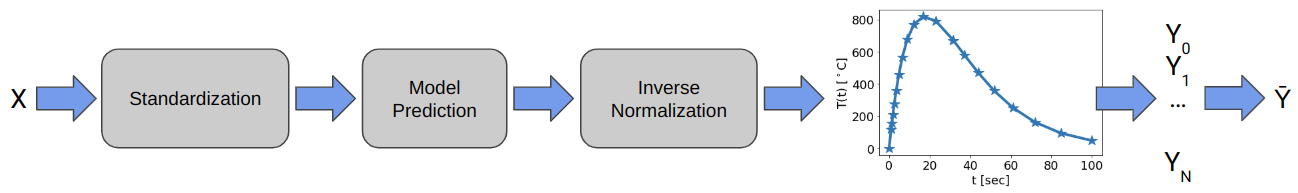
\includegraphics[width=0.7\linewidth]{figures/data-prediction-fnn}
  \caption{Visualization of time-evolution prediction using FNN.}
  \label{fig:data-reg2}
\end{figure}

% LSTM MODEL
The third method uses LSTMs to predict the whole time evolution of the highest temperature in the capsule at once.
The data handling process for this method is summarized in Figure \ref{fig:data-lstm}.
The first step in the LSTM implementation transforms the problem into a supervised one, as described in Section \ref{sec:lstm}.
The number of look-forward steps is fixed to 40, while the network optimization defines the number of look-back steps.
Then, the samples are normalized and separated into an 80-20 training-testing split.

\begin{figure}[htbp!] %htbp! or H
  \centering
  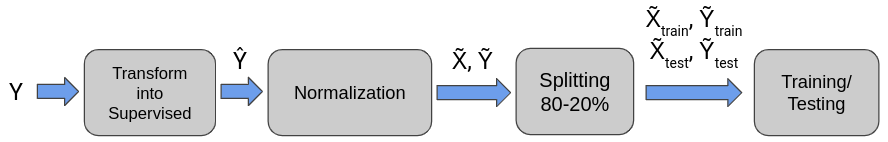
\includegraphics[width=0.7\linewidth]{figures/data-pross-lstm}
  \caption{Data handling process for the time-evolution prediction using LSTMs.}
  \label{fig:data-lstm}
\end{figure}

The network has four LSTM layers and one dense output layer.
The network optimization defines the number of nodes in the LSTM layers, the number of look-back steps, and the training batch size.
The training of the network uses the Adam optimizer to minimize the \gls*{MAE}, and the learning rate is fixed to $5 \times 10^{-4}$.
Bayesian optimization using Gaussian processes (Section \ref{sec:opt}) optimized the network by maximizing the $R^2$ score.
The optimal configuration was 167, 98, 62, and 139 nodes for the hidden layers, six look-back steps, and a batch size of 12.
Once the model is trained, the model can predict the outcome of the transient by reading the material properties of a specific sample and coefficients defining the delayed heating, as shown in Figure \ref{fig:data-reg3}.
Then, the trained model predicts $\tilde{Y}$ that is de-normalized into $\hat{Y}$, which is used to reconstruct the time-series $Y$ and translated into the output variable $\bar{Y}$.

\begin{figure}[htbp!] %htbp! or H
  \centering
  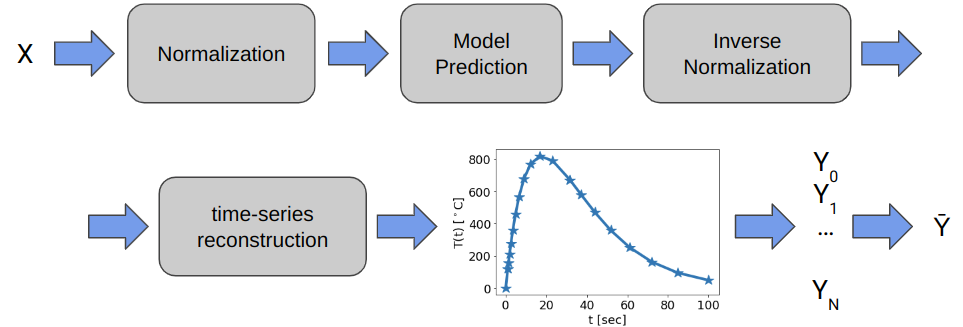
\includegraphics[width=0.7\linewidth]{figures/data-prediction-lstm}
  \caption{Visualization of time-evolution prediction using LSTM.}
  \label{fig:data-reg3}
\end{figure}


\subsection{Strategy Comparison}
\label{sec:comp}

This section compares the performance of the two different strategies described in Section \ref{sec:datapros}.
The first strategy relies on classification methods to predict the state of the experiment's capsule.
The second strategy uses several approaches to predict the time evolution of the capsule temperature.

% fairhurst-agosta_machine_2022
Table \ref{tab:results-1} summarizes the main results of the classification problem for the testing dataset.
In terms of accuracy, LogR and FNN are the worst and best-performing methods, respectively.
All the methods show an accuracy higher than 0.96.
When focusing on the recall, both methods show again the worst and best performances.
LogR is the only method with a recall lower than 0.97.
The last comparison metric is the model training time.
The FNN took longer to train than the other models.
All the methods are trained quickly in under 1 second, except for FNN which took almost half a minute.
This training time does not include the hyperparameter tuning, which takes a substantially longer time, in the order of 10 to 20 minutes.
Overall, all these values are small and acceptable, and the FNN remains the preferred method.
Figure \ref{fig:cnfm} displays the confusion matrix for the LogR and the FNN cases.
The comparison of both results shows a clear improvement from LogR to FNN in the mislabeled samples.

% Table
\begin{table}[htbp!]
  \centering
  \caption{Performance metrics of the machine learning techniques for the classification problem.}
  \label{tab:results-1}
  \begin{tabular}{lccc}
  % \begin{tabularx}{\textwidth}{@{}*4{>{\hsize=.56\hsize\centering\arraybackslash}X}@{}}
    \toprule
    Method & Accuracy & Recall & Train Time [sec] \\
    \midrule
    DT      & 0.9902 & 0.9705 & $<$1 \\
    FNN     & 0.9963 & 0.9937 & 27 \\
    KNN     & 0.9860 & 0.9747 & $<$1 \\
    LogR    & 0.9655 & 0.9116 & $<$1 \\
    RF      & 0.9911 & 0.9726 & $<$1 \\
    SVM     & 0.9841 & 0.9832 & $<$1 \\
    \bottomrule
  \end{tabular}
\end{table}

\begin{figure}[htbp!] %or H 
    \centering
    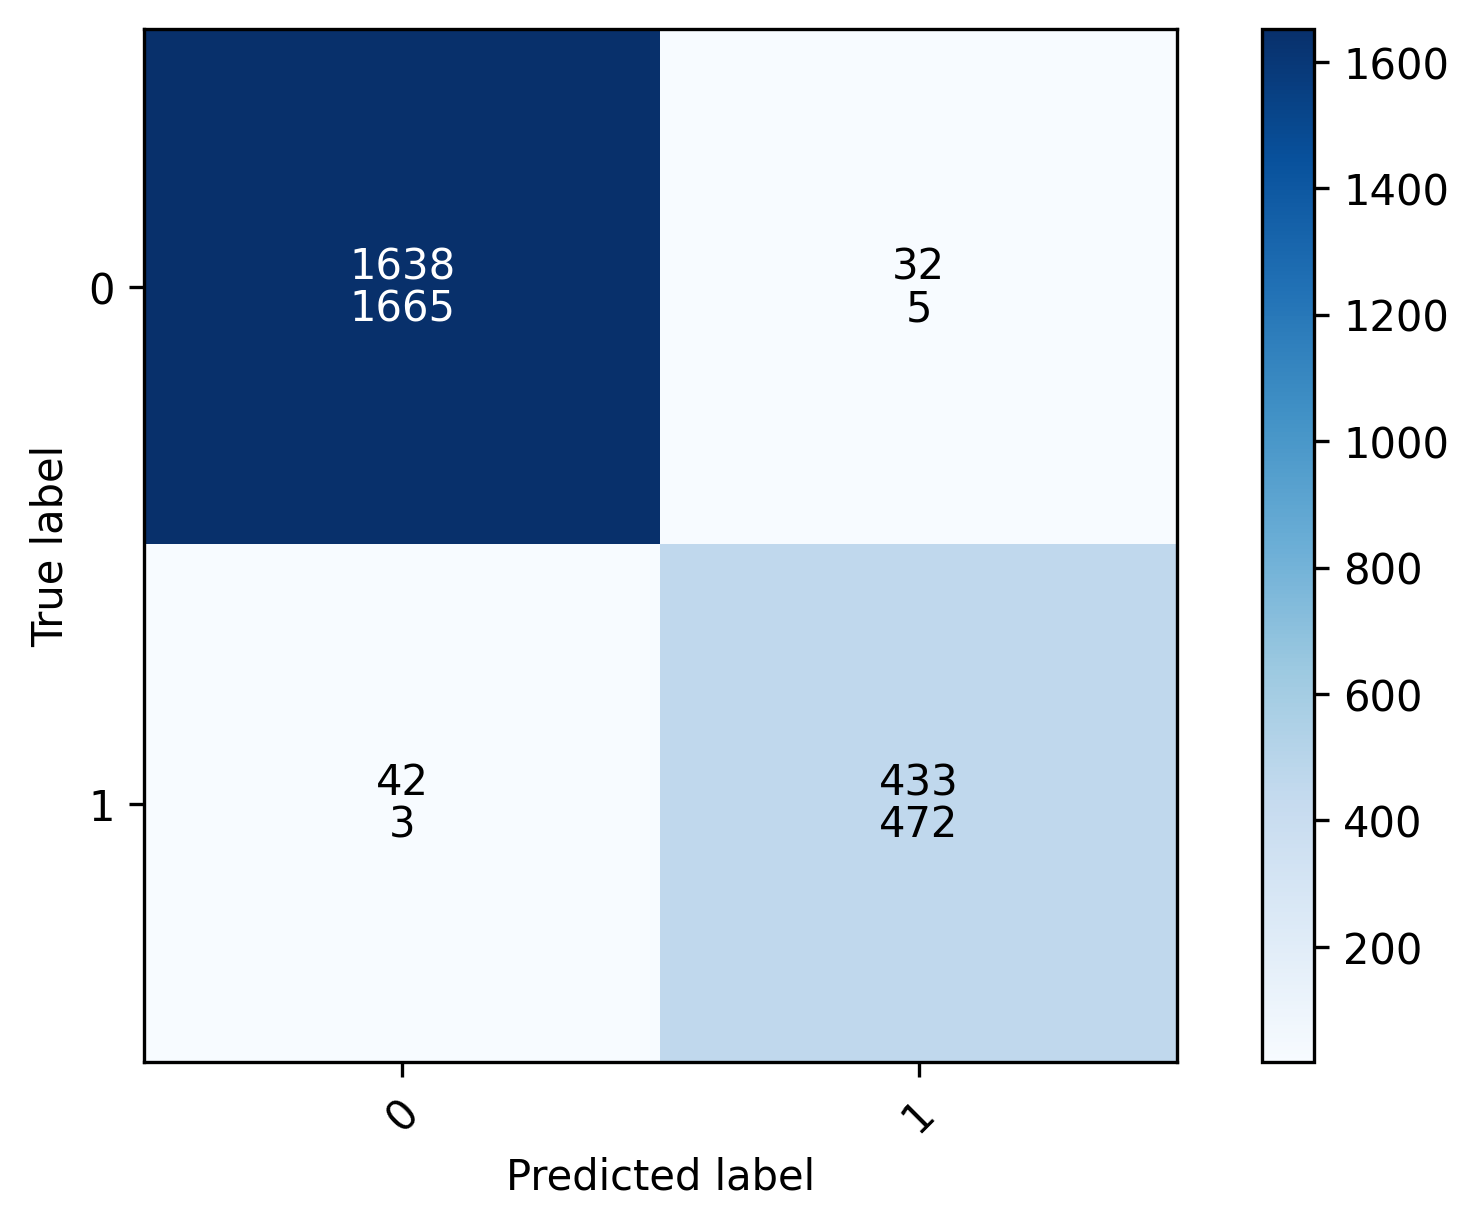
\includegraphics[width=0.45\linewidth]{figures/classification_cnfm.png}
    \hfill
    \caption{Confusion matrix for the LogR (top) and FNN (bottom) cases. The labels 1/0 represent \textit{melt}/\textit{does not melt}.}
    \label{fig:cnfm}
\end{figure}

% fairhurst-agosta_machine_2_2022
Table \ref{tab:results-2} summarizes the main results of the time-evolution prediction problem for the testing dataset.
Overall, all methods achieved high accuracy and recall.
DTR shows the worst performance, with an accuracy lower than 0.99, and a recall lower than 0.97.
The FNN shows the highest accuracy and recall.
In terms of melting-time relative error, all the methods show large maximum relative errors, in the order of 30 to 50\%.
The mean relative error, on the other hand, is low for the FNN and the LSTM.
The RFR shows the worst performance, with a mean relative error close to 18\%.

% show training time
% Table
\begin{table}[htbp!]
  \centering
  \caption{Performance metrics of the different methods for the time-evolution prediction problem.}
  \label{tab:results-2}
  \begin{tabular}{lcccc}
  % \begin{tabularx}{\textwidth}{@{}*5{>{\hsize=.56\hsize\centering\arraybackslash}X}@{}}
    \toprule
    Method & Accuracy & Recall & Mean t$_{Melt}$ Rel. Error & Max. t$_{Melt}$ Rel. Error \\
    \midrule
    DTR      & 0.9889 & 0.9617 &                     8.2 \% &                    43.0 \% \\
    FNN      & 0.9976 & 1.0000 &                     1.0 \% &                    31.1 \% \\
    LSTM     & 0.9952 & 0.9933 &                     3.4 \% &                    29.0 \% \\
    RFR      & 0.9928 & 0.9797 &                    17.6 \% &                    45.1 \% \\
    \bottomrule
  \end{tabular}
\end{table}

Regarding the accuracy, recall, and mean melting-time relative error, the FNN is the best-performing method.
LSTM has high accuracy and recall and a low mean melting-time relative error.
Hence, it is the second best performing method.
DTR and RFR are the worst-performing methods.

Depending on the final application of the models, one may benefit from choosing the regression or the deep-learning methods.
Although the tables do not present the training times, FNN and LSTM required optimization, which translates into high training times.
Another desirable feature can be visualization.
Deep-learning methods work in a ``black box"-fashion, where the visualization of the network does not provide much insight to the scientist.
The regression of the non-linear fitting coefficients, on the other hand, is a method relatively simple and easy to visualize.
However, the method contains multiple steps, wherein uncertainties could be introduced, deteriorating the quality of the final result.

Figure \ref{fig:t-evol} displays some examples of time-evolution prediction using the three approaches.
It is possible to discern the time discretization in all the curves.
As machine learning algorithms have to predict the temperature evolution, it simplifies the learning process to reduce the number of time steps.
For the most part, when trying to determine whether the capsule melts or not, a coarse time discretization is still enough to capture this behavior.
When trying to predict the exact time when the capsule melts, such a coarse time discretization introduces considerably large errors for some of the testing samples, which is the cause of the large maximum t$_{Melt}$ relative errors shown in Table \ref{tab:results-2}.  
Overall, the predicted values approximate well the expected values, and hence the mean t$_{Melt}$ relative error is low, as shown in Table \ref{tab:results-2}.

\begin{figure}[htbp!] % or H
  \centering
  \begin{subfigure}[b]{0.49\textwidth}
    \centering
    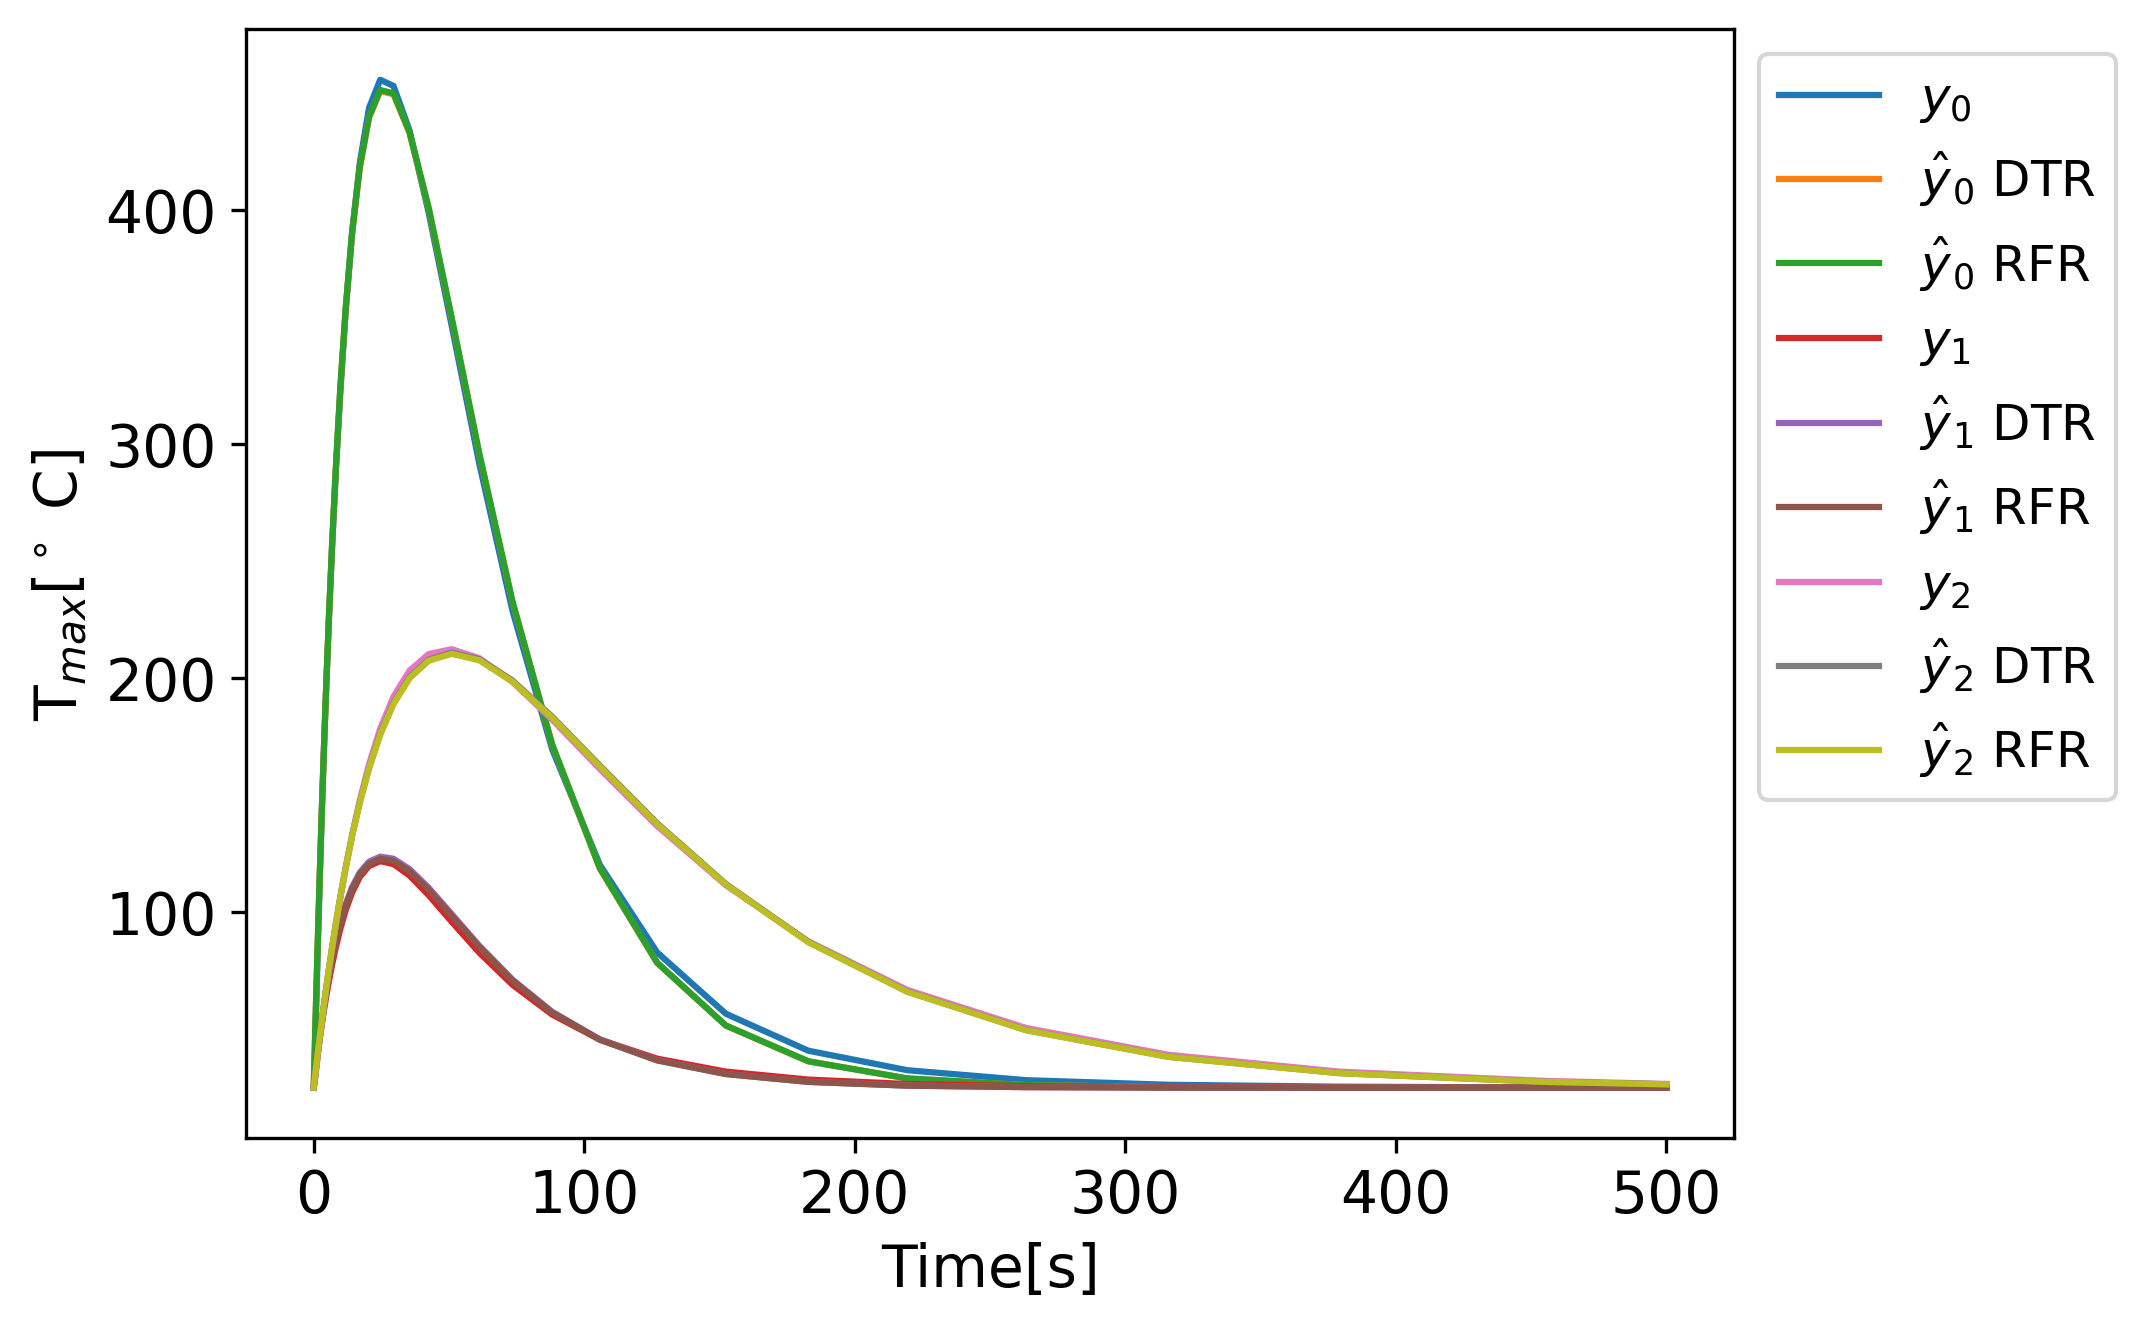
\includegraphics[width=1.0\textwidth]{figures/regression2_good_inspect}
    \caption{Regression of non-linear fitting coefficients.}
  \end{subfigure}
  \hfill
  \begin{subfigure}[b]{0.49\textwidth}
    \centering
    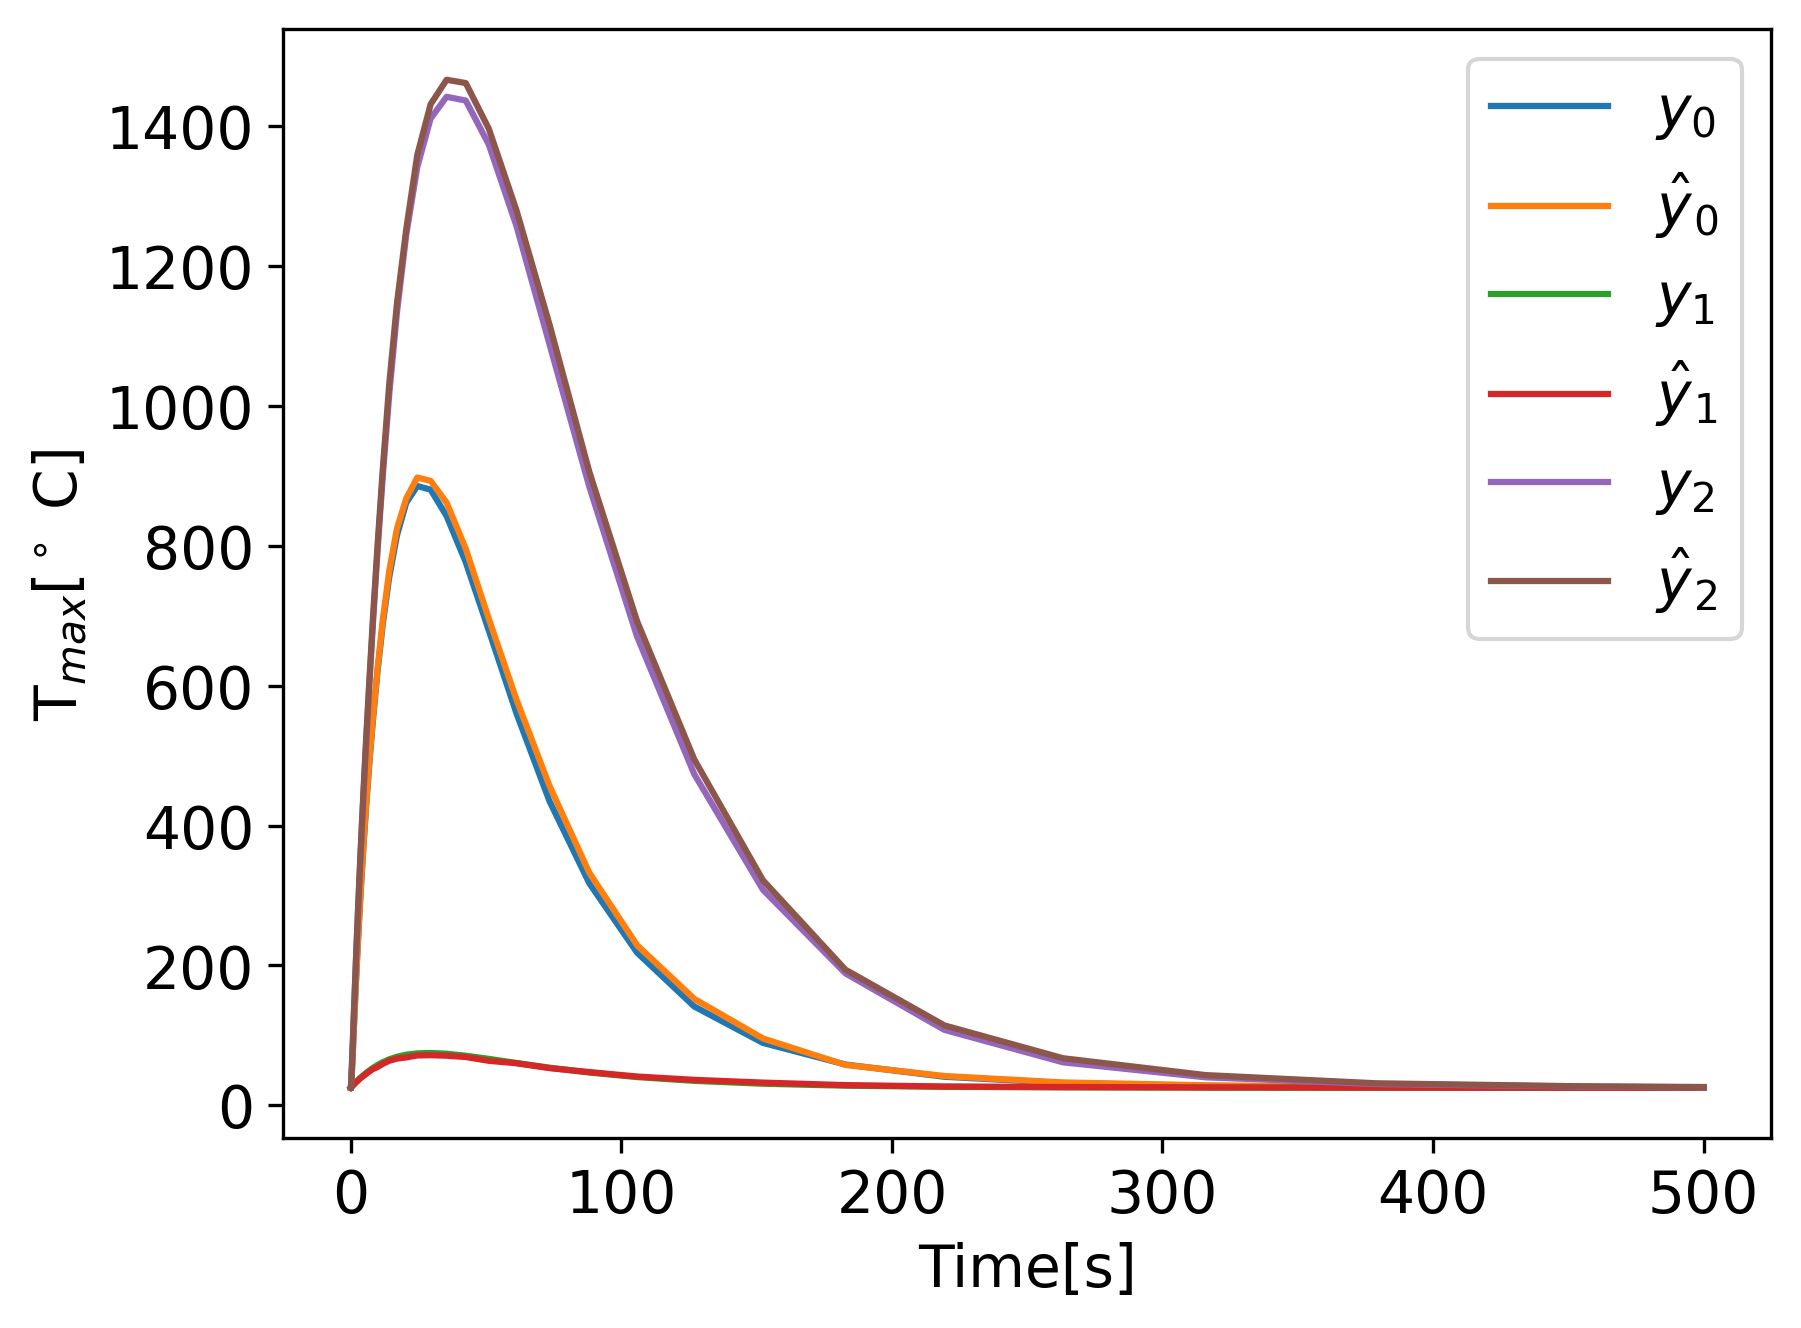
\includegraphics[width=0.85\textwidth]{figures/time_fnn_inspect}
    \caption{FNN.}
  \end{subfigure}
  \par
  \begin{subfigure}[b]{0.49\textwidth}
    \centering
    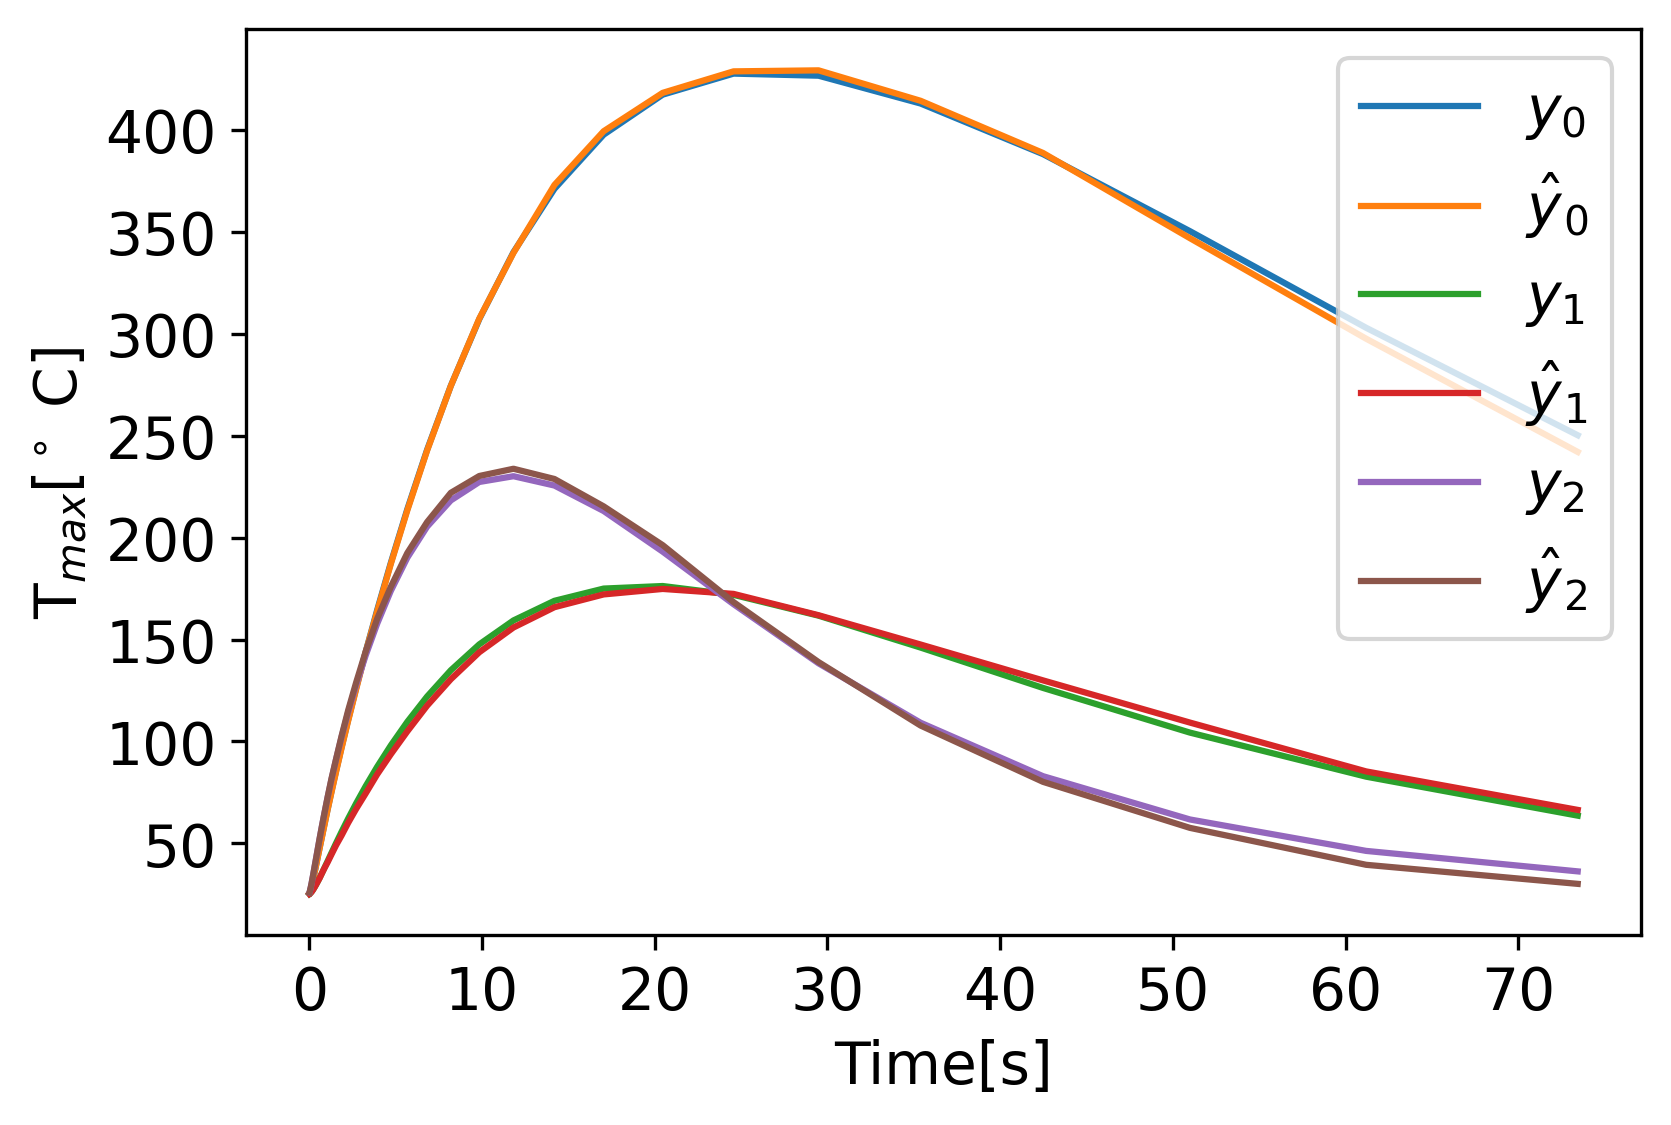
\includegraphics[width=0.85\textwidth]{figures/time_lstm_inspect}
    \caption{LSTM.}
  \end{subfigure}
  \caption{Example of time-evolution prediction using the three approaches.}
  \label{fig:t-evol}
\end{figure}


\subsection{Non-dimensional thermal properties}

This section investigates an alternative for the classification problem to reduce the model complexity.
Instead of using all the material thermal properties (three features) to train and test the model, the model uses only one feature: the thermal diffusivity
\begin{align}
\alpha &= \frac{k}{\rho c_p}
\end{align}
where $k$ is the thermal conductivity, $\rho$ is the density, and $c_p$ is the specific heat capacity.
The motivation for this study is that reducing the number of features should allow the model to be trained more ``easily''.
The more features the model has, the more complex the relationship between input and outputs becomes.
By reducing the number of features, the input/output relationship should become simpler, and hence the model is easier to train.
This study intends to confirm/refuse this hypothesis by using the same data from the study from previous section.

Table \ref{tab:res-pre-alpha} summarizes the main results of the classification problem for the testing dataset.
In terms of accuracy, LogR and DT are the worst and best-performing methods, respectively.
All the methods show an accuracy higher than 0.95.
When focusing on the recall, both methods show again the worst and best performances.
LogR is the only method with a recall lower than 0.95.
The last comparison metric is the model training time.
The FNN took longer to train than the other models.
All the methods are trained quickly in under 1 second, except for FNN which took 1 minute.
However, all these values are very small and acceptable, and the FNN remains as the preferred method.
Figure \ref{fig:pre-cnfm-alpha} displays the confusion matrix for the LogR and the DT cases.
The comparison of both results shows a clear improvement from LogR to DT in the mislabeled samples.

A comparison between the results from Section \ref{sec:comp} and these results shows that all methods perform better when considering all the thermal properties as features.
Although condensing the thermal properties into one value seems to decrease the complexity of the model, the accuracy and recall of the model worsen slightly.
This is because using the thermal diffusivity as a feature causes the model to lose some resolution, as the thermal diffusivity ``hides'' the variations in the thermal properties.
Figure \ref{fig:pre-cnfm-alpha-2} helps to visualize this phenomenon.
For example, if the model is trained with materials with extreme values - i.e., lithium and iridium, most of the materials' thermal properties fall within the lithium and iridium bounds.
If sodium becomes the testing sample, for the model trained with all the thermal properties, its thermal properties are within the bounds of the training data.
On the other hand, for the model trained with the thermal diffusivity, the sodium testing sample falls outside the bounds of the training data, deteriorating the model prediction.
Although these results suggest that training the model with all the thermal properties is best, the results do not worsen considerably, and more investigation should confirm/refuse this analysis.

% Table
\begin{table}[htbp!]
  \centering
  \caption{Performance metrics of the machine learning techniques for the classification problem using thermal diffusivity as a feature.}
  \label{tab:res-pre-alpha}
  \begin{tabular}{lccc}
    \toprule
    Method & Accuracy & Recall & Train Time [sec] \\
    \midrule
    DT      & 0.9883 & 0.9797 & $<$1 \\
    FNN     & 0.9739 & 0.9684 &   60 \\
    KNN     & 0.9776 & 0.9684 & $<$1 \\
    LogR    & 0.9585 & 0.8736 & $<$1 \\
    RF      & 0.9855 & 0.9729 & $<$1 \\
    SVM     & 0.9692 & 0.9503 & $<$1 \\
    \bottomrule
  \end{tabular}
\end{table}

\begin{figure}[htbp!] %or H 
    \centering
    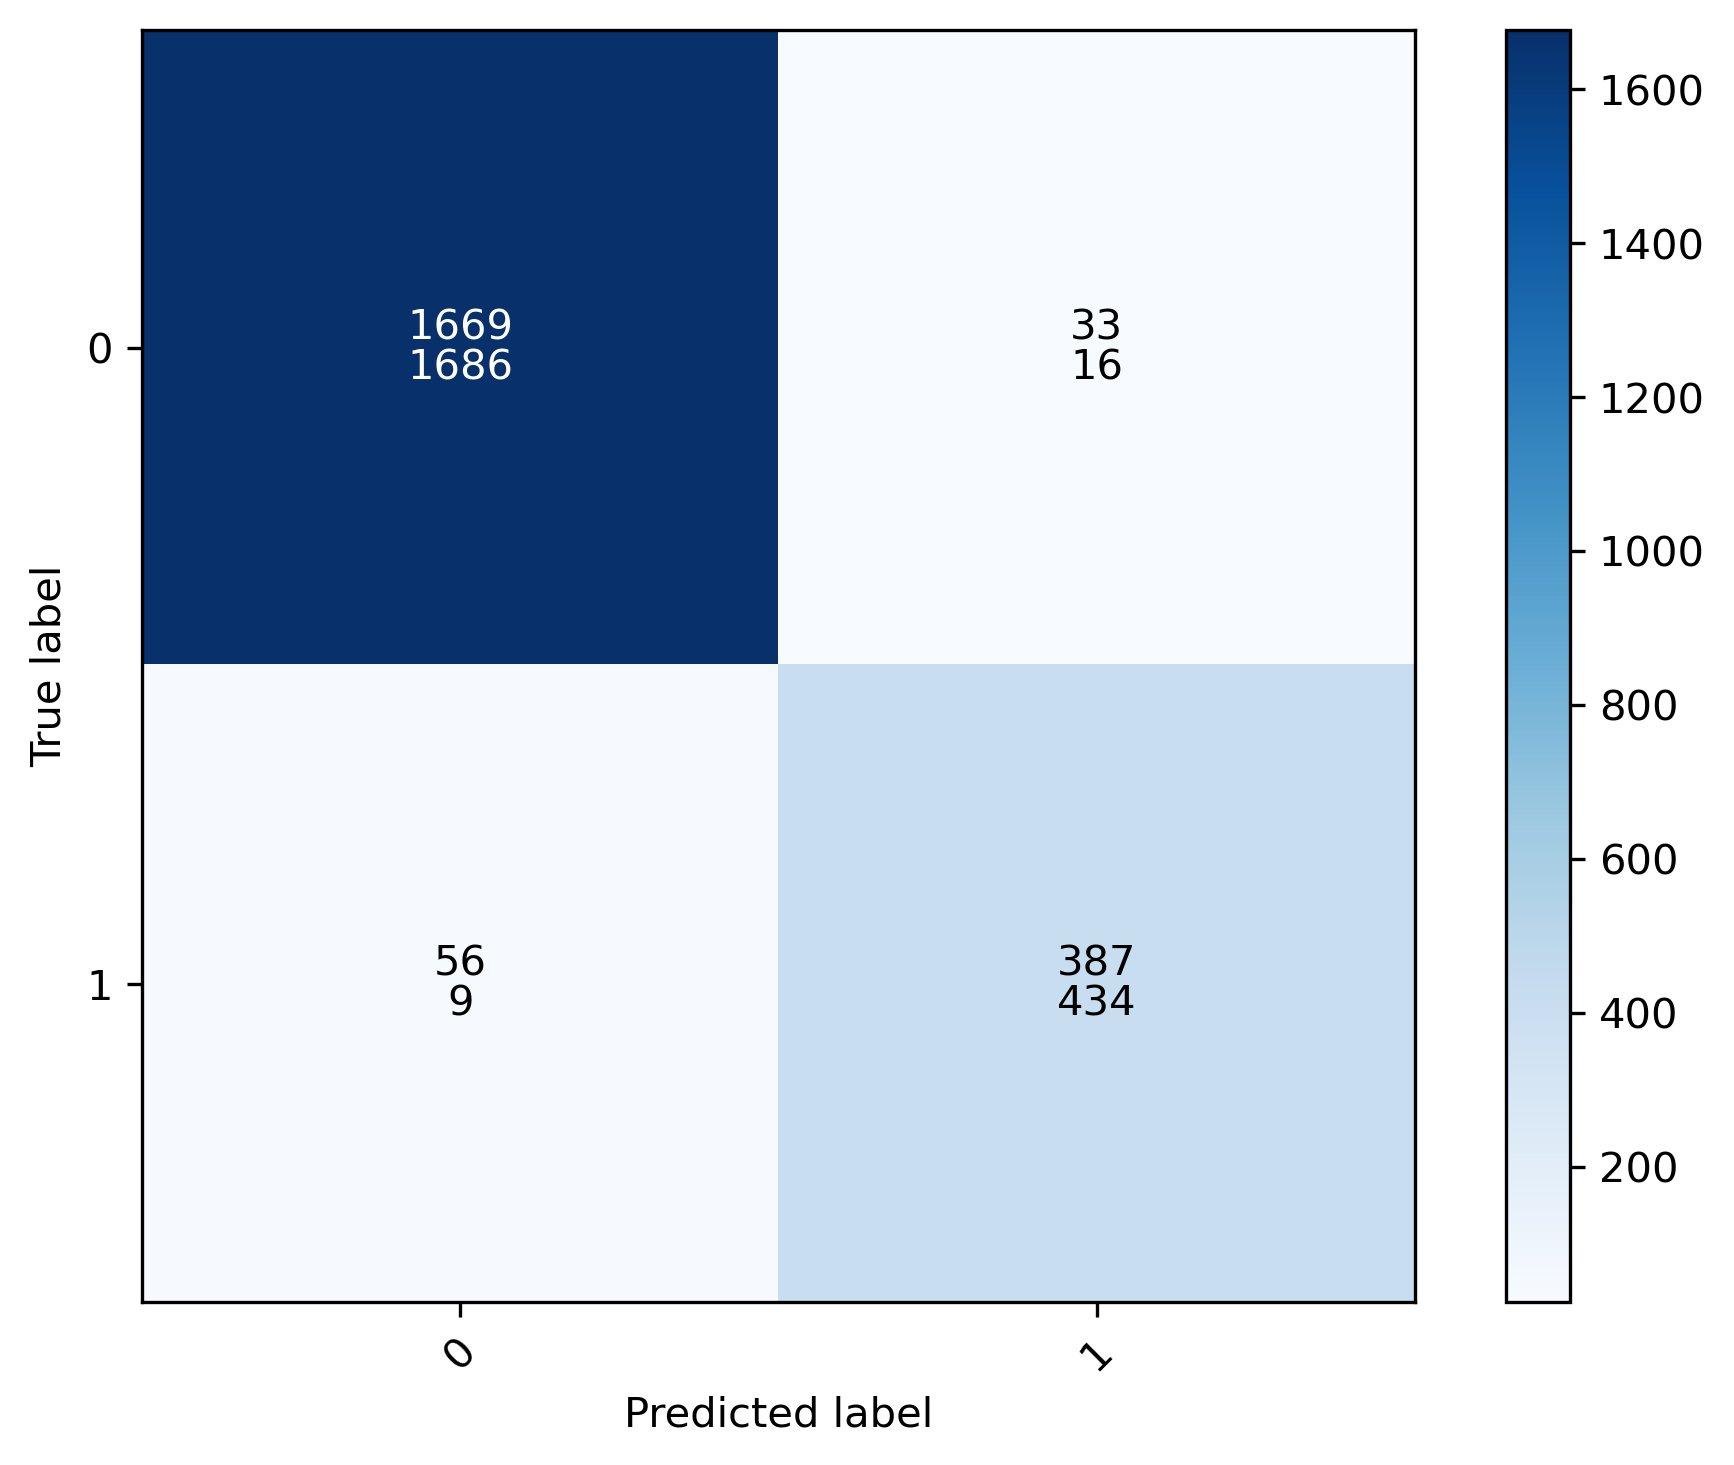
\includegraphics[width=0.45\linewidth]{figures/classification-alpha_cnfm}
    \hfill
    \caption{Confusion matrix for the LogR (top) and DT (bottom) cases. The labels 1/0 represent \textit{melt}/\textit{does not melt}.}
    \label{fig:pre-cnfm-alpha}
\end{figure}

\begin{figure}[htbp!] %or H 
    \centering
    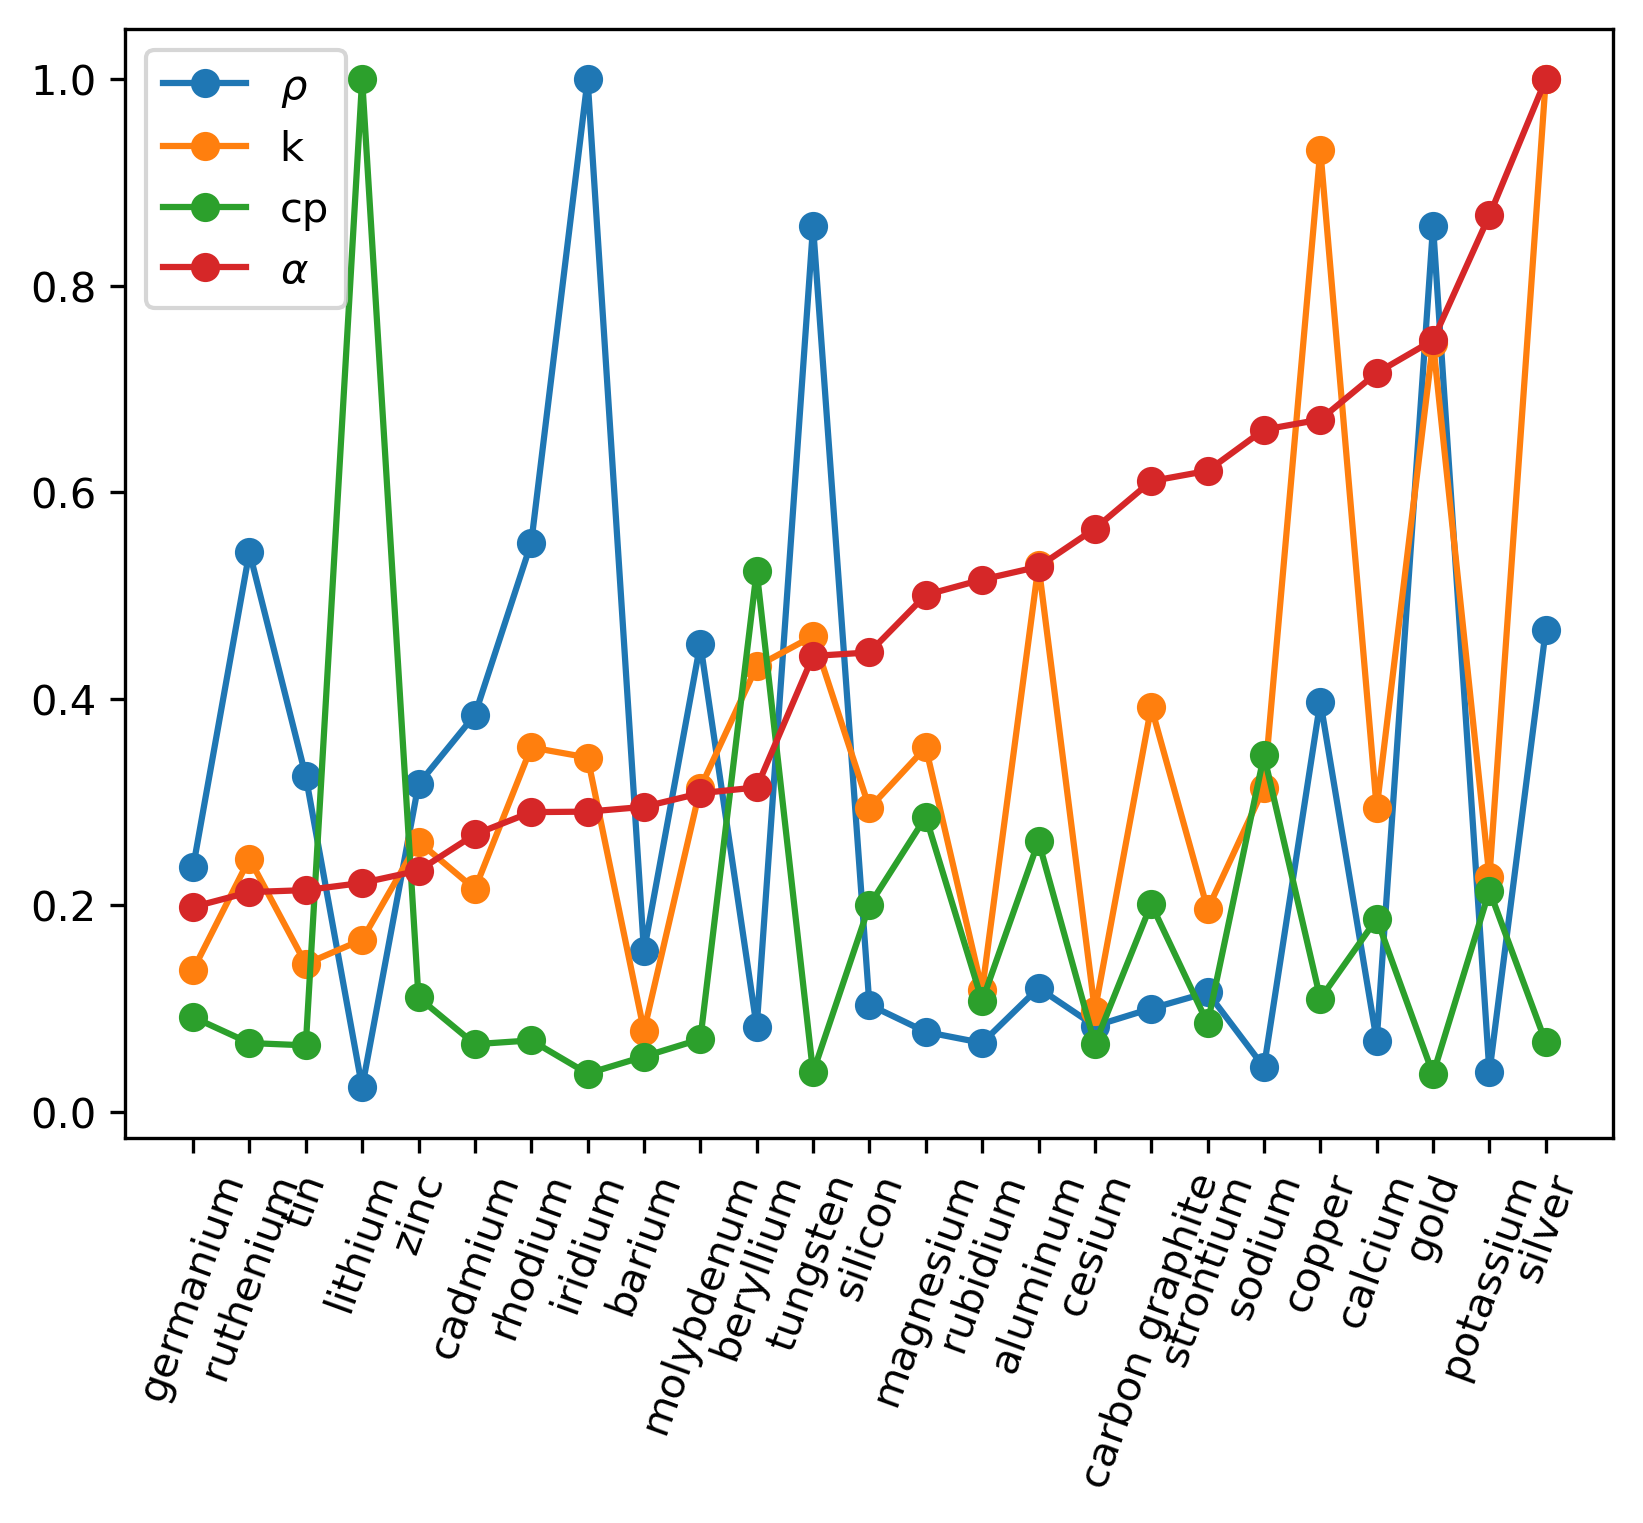
\includegraphics[width=0.65\linewidth]{figures/alpha}
    \hfill
    \caption{Thermal properties for selected materials. Values are normalized to maximum values of materials in the shown range.}
    \label{fig:pre-cnfm-alpha-2}
\end{figure}


\subsection{Synthetic Materials}
\label{sec:syn-mat}

% Increase statistics
This section investigates the training and testing of the models using synthetic thermal properties.
The motivation for this study is to augment the training and testing data to broaden the range of applicability of the data-based model to more possible irradiated materials.
These synthetic thermal properties are generated by randomly sampling each thermal property assuming a uniform distribution between the minimum and maximum values from the list of 82 real materials included in Appendix \ref{ap:mat_props}.

% New data format
The thermal properties values correspond to 200 synthetic materials and 82 real materials.
$q_0$ comprises 18 uniformly distributed values between 10$^7$ and 10$^8$ W/m$^3$, and 20 between 10$^8$ and 5 $\times$ 10$^8$ W/m$^3$, totaling 38 unique values.
$\tau$ comprises five uniformly distributed values between 20 and 100 seconds.
The combination of all these variables leads to a total of 53390 samples.
However, some of the samples were discarded because the simulations did not reach completion for uninvestigated reasons, and the total number of usable samples was 40550.

Table \ref{tab:res-pre-synt} summarizes the main results of the classification problem for the testing dataset.
In terms of accuracy, LogR and FNN are the worst and best-performing methods, respectively.
All the methods show an accuracy higher than 0.96.
When focusing on the recall, both methods show again the worst and best performances.
LogR is the only method with a recall lower than 0.94.
The last comparison metric is the model training time.
The FNN took longer to train than the other models.
All the methods are trained quickly in under 1 second, except for FNN which took over 4 minutes.
However, all these values are very small and acceptable, and the FNN remains as the preferred method.
Figure \ref{fig:pre-cnfm-syn} displays the confusion matrix for the LogR and the FNN cases.
The comparison of both results shows a clear improvement from LogR to FNN in the mislabeled samples.

A comparison between the results from Section \ref{sec:comp} and these results shows that all methods perform better when considering real data for the thermal properties.
Figure \ref{fig:pre-syn-mats} shows the relationship between thermal properties for selected real materials.
The plots show certain correlation between the different thermal properties.
The one most obvious is the relationship between heat capacity and density which follows a $1/x$-shape.
For the other thermal properties, the correlations are not so easily discernible.
However, a clear aspect is that the plotted values are not uniformly distributed, but concentrated in specific areas of the domain.
For example, the relationship between heat capacity and thermal conductivity shows only a few points above 1000 J/kg/K, while the rest of them are concentrated below 500 J/kg/K and below 100 W/m/K.
These figures prove that assuming a uniform distribution for the thermal properties between minimum and maximum values is not appropriate.
In conclusion, this assumption causes the models to learn the correlations between input features in areas of the domain that are not representative of reality and should be avoided.

% Table
\begin{table}[htbp!]
  \centering
  \caption{Performance metrics of the machine learning techniques for the classification problem.}
  \label{tab:res-pre-synt}
  \begin{tabular}{lccc}
    \toprule
    Method & Accuracy & Recall & Train Time [sec] \\
    \midrule
    DT      & 0.9861 & 0.9433 &   $<$1 \\
    FNN     & 0.9948 & 0.9808 & 4'26'' \\
    KNN     & 0.9847 & 0.9452 &   $<$1 \\
    LogR    & 0.9676 & 0.8528 &   $<$1 \\
    RF      & 0.9898 & 0.9525 &   $<$1 \\
    SVM     & 0.9938 & 0.9771 &   $<$1 \\
    \bottomrule
  \end{tabular}
\end{table}

\begin{figure}[htbp!] %or H 
    \centering
    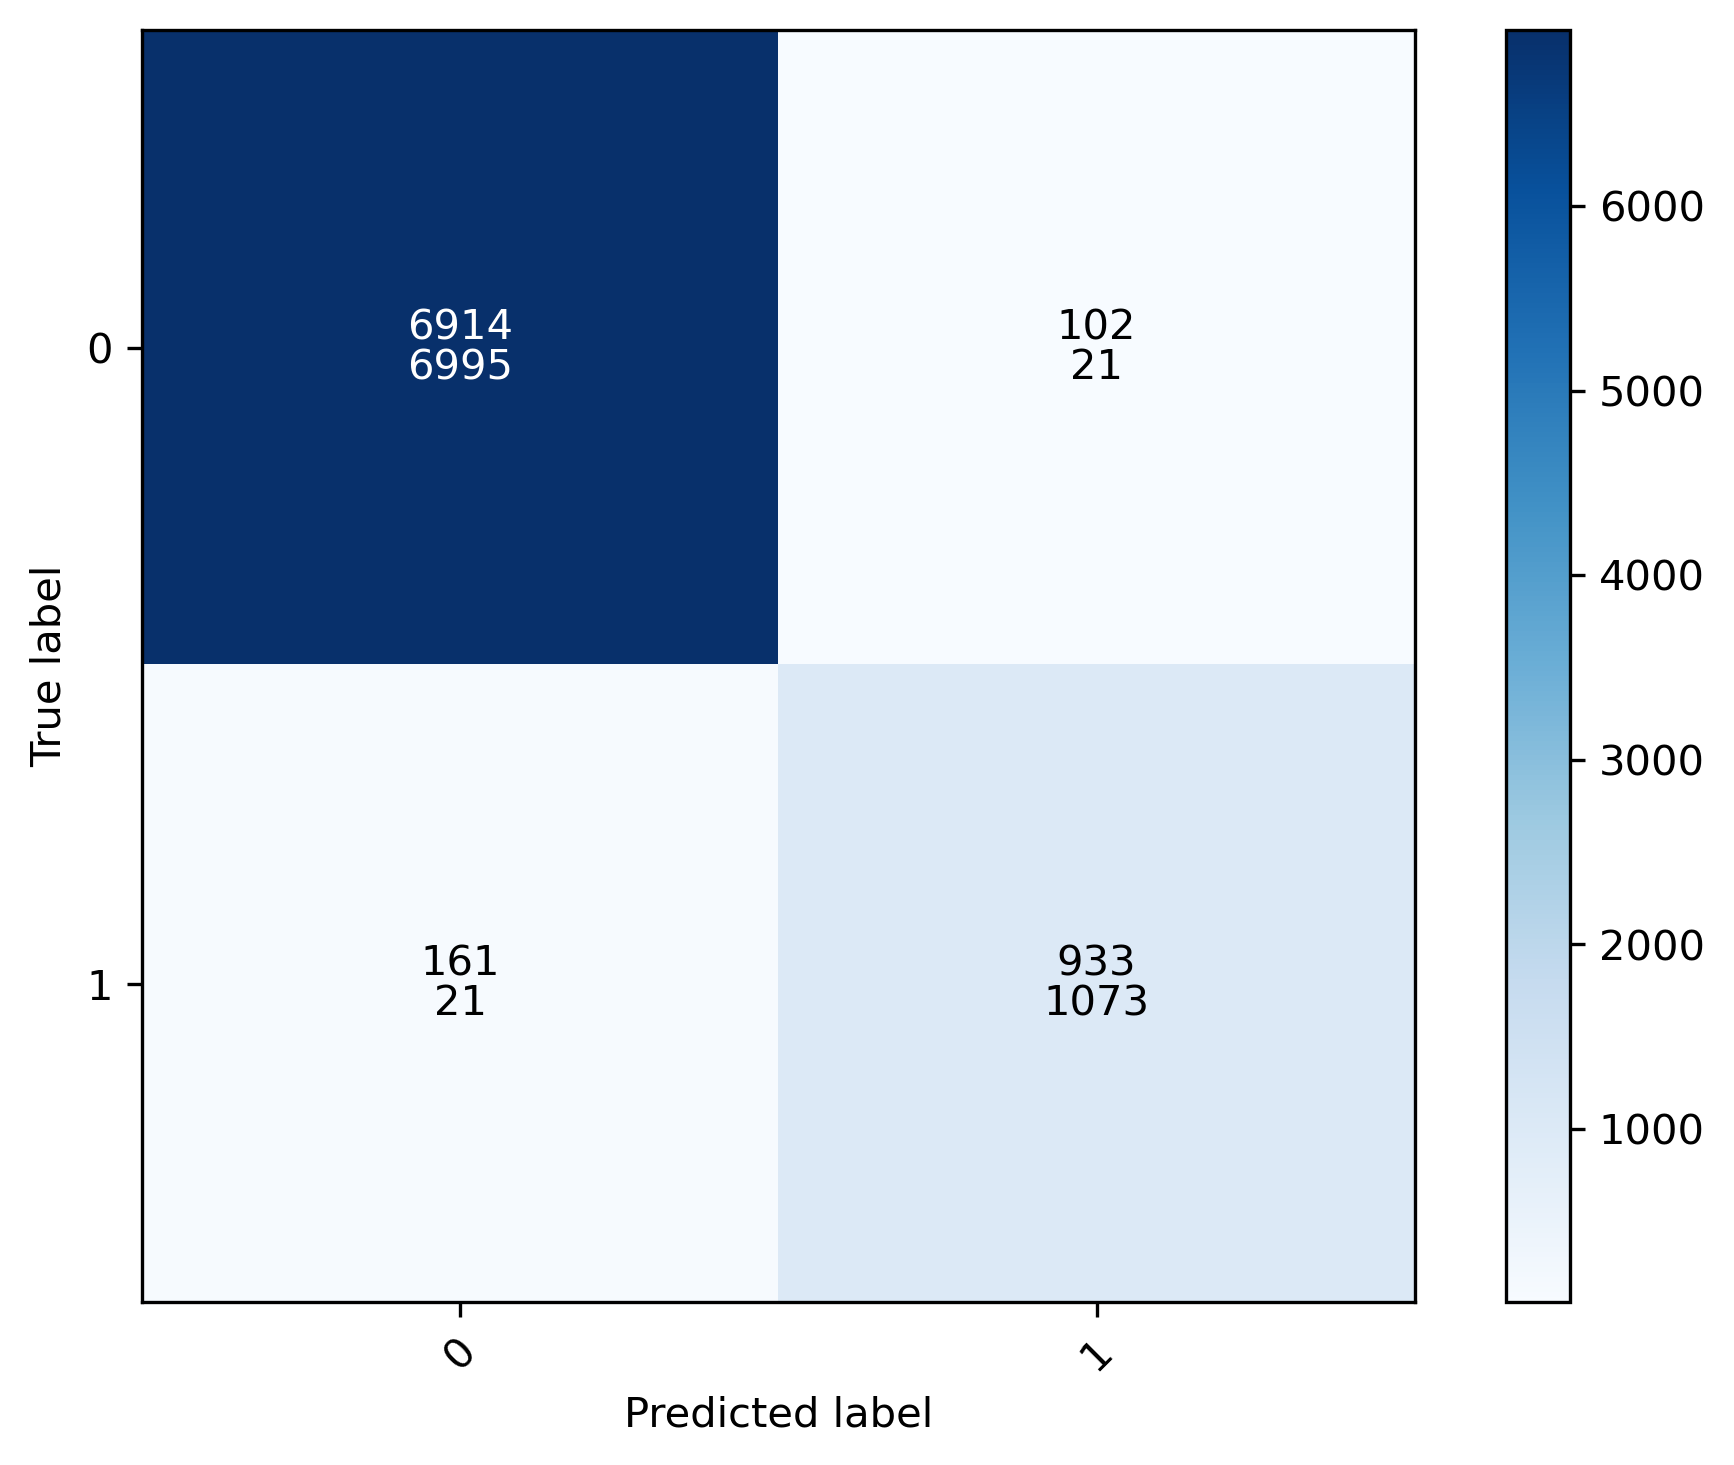
\includegraphics[width=0.45\linewidth]{figures/classification-synth_cnfm}
    \hfill
    \caption{Confusion matrix for the LogR (top) and FNN (bottom) cases. The labels 1/0 represent \textit{melt}/\textit{does not melt}.}
    \label{fig:pre-cnfm-syn}
\end{figure}

\begin{figure}[htbp!] % or H
  \centering
  \begin{subfigure}[b]{0.49\textwidth}
    \centering
    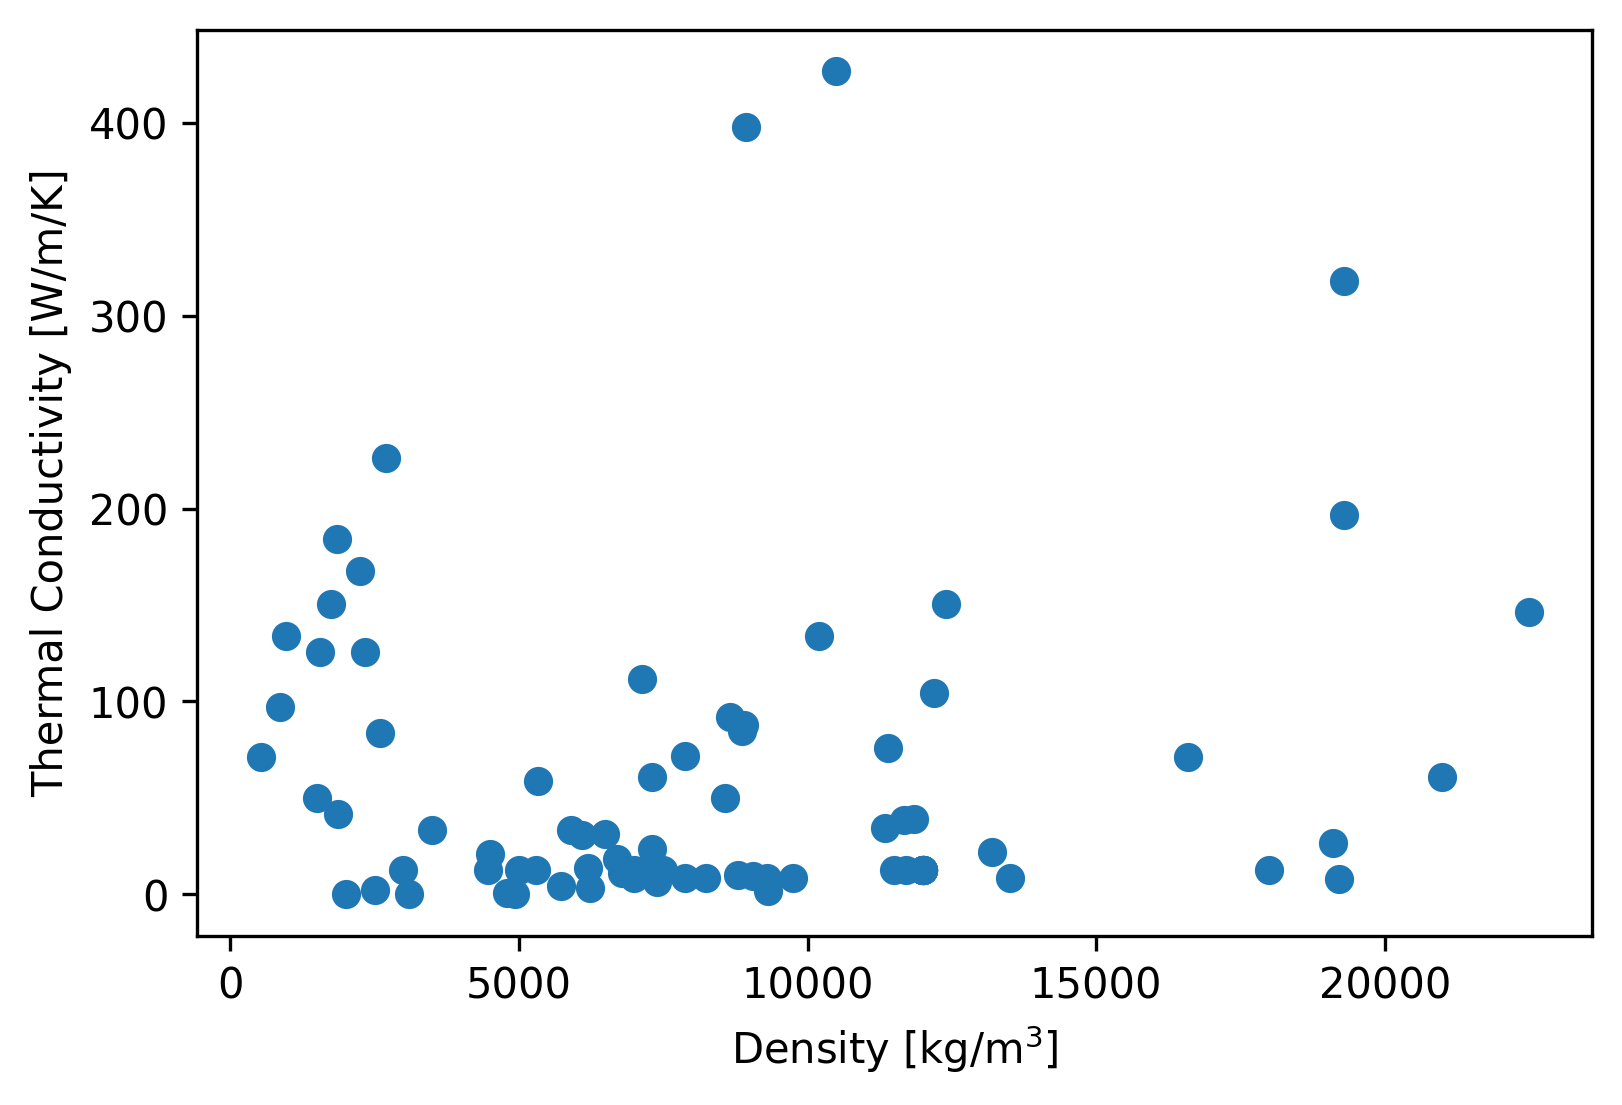
\includegraphics[width=0.85\textwidth]{figures/rho_k}
    \caption{Thermal conductivity vs. density.}
  \end{subfigure}
  \hfill
  \begin{subfigure}[b]{0.49\textwidth}
    \centering
    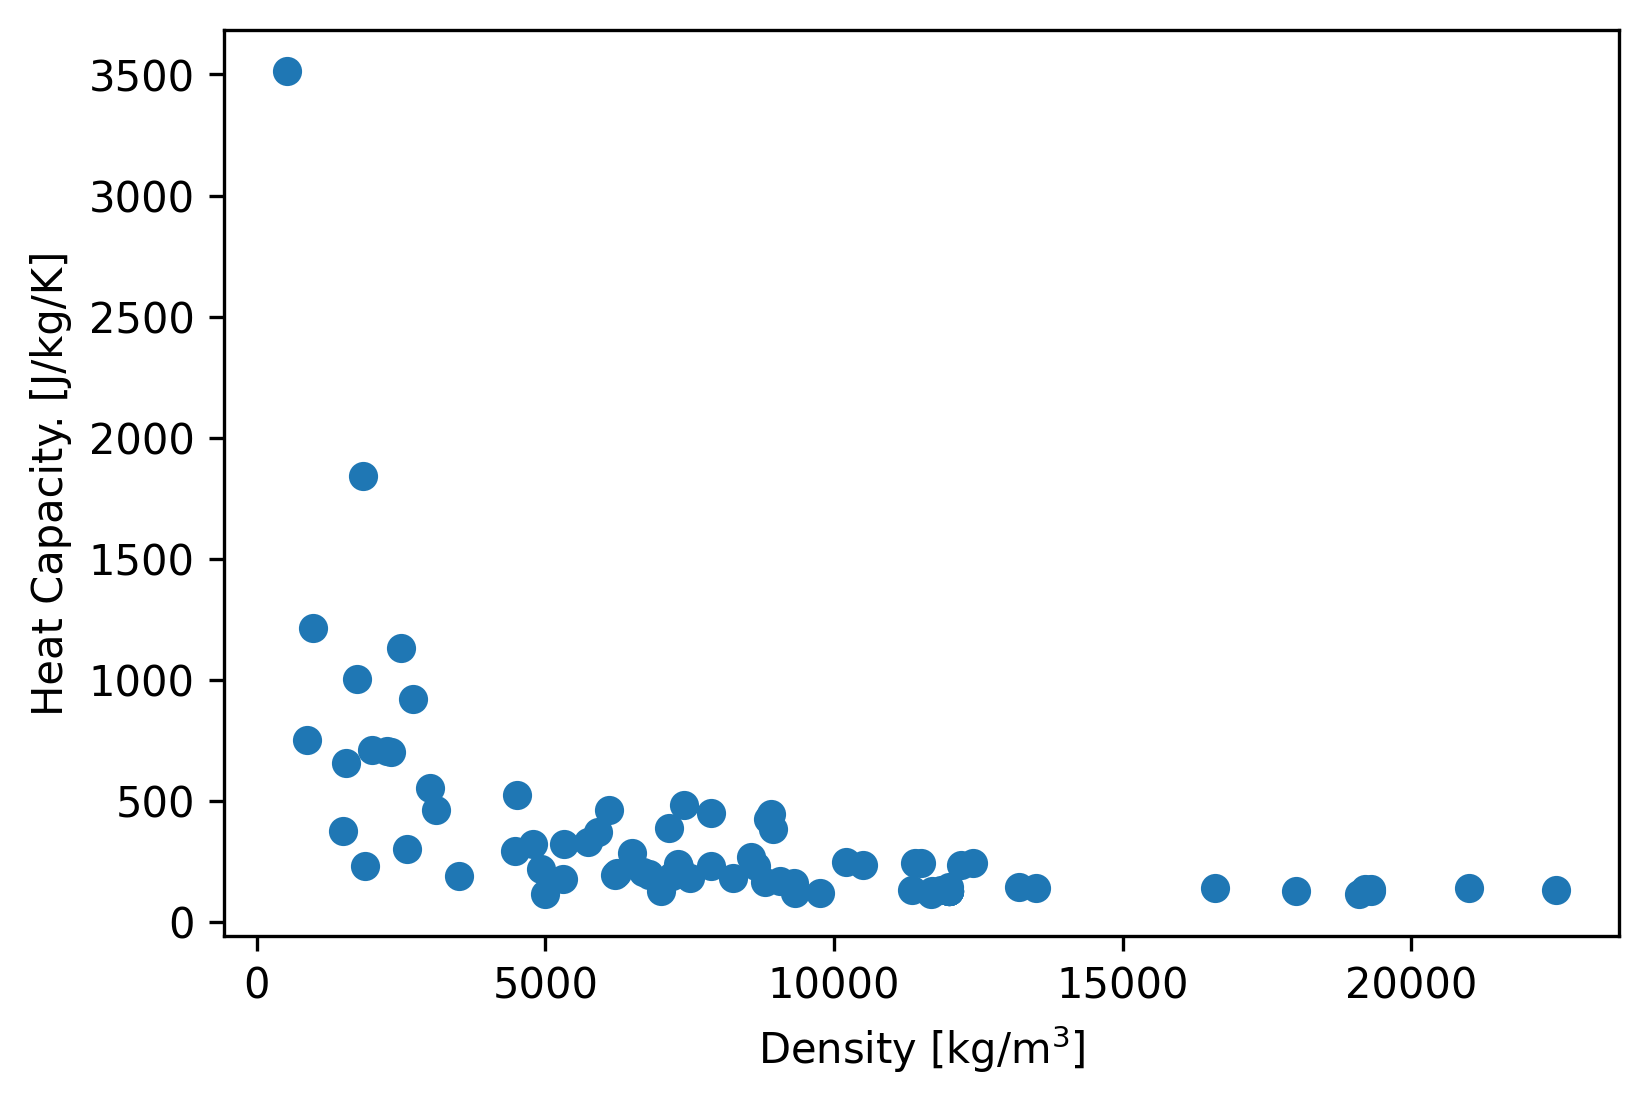
\includegraphics[width=0.85\textwidth]{figures/rho_cp}
    \caption{Heat capacity vs. density.}
  \end{subfigure}
  \par
  \begin{subfigure}[b]{0.49\textwidth}
    \centering
    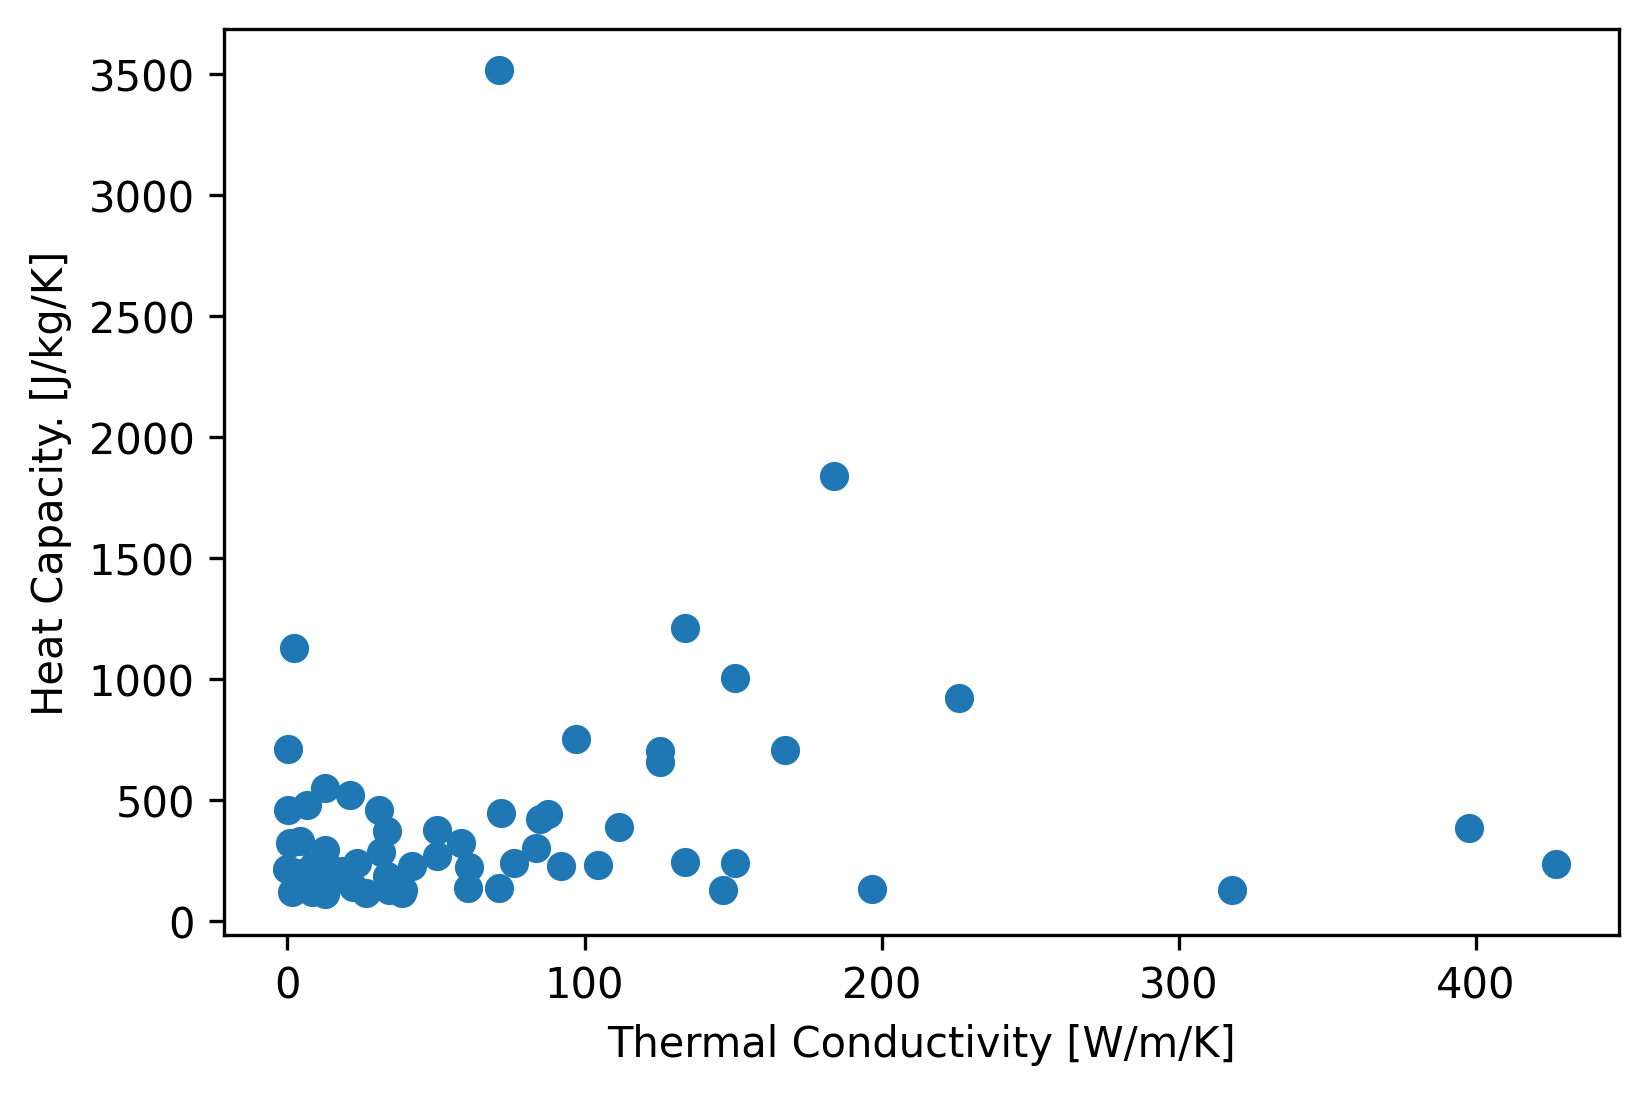
\includegraphics[width=0.85\textwidth]{figures/k_cp}
    \caption{Heat capacity vs. thermal conductivity.}
  \end{subfigure}
  \caption{Relationship between thermal properties for selected materials.}
  \label{fig:pre-syn-mats}
\end{figure}


\section{Source Decomposition}
\label{sec:sou_decomp}

% https://dsp.stackexchange.com/questions/66428/how-to-compute-laplace-transform-in-python
% https://stackoverflow.com/questions/38316225/numerical-laplace-transform-python
% https://stackoverflow.com/questions/58193209/function-to-determine-the-frequency-of-a-sinusoid
% https://physics.uncg.edu/hellen/pade_laplace/pade-laplace.html
% This one is very close: https://randorithms.com/2020/03/08/exponential-sum-fits.html

The analyses described above assume that the experiment produces heat with a source of shape $q_0 e^{-t/\tau}$.
Further inspection of the delayed heating results from Chapter \ref{ch:delayedheat} shows that the experiment heat does not follow the shape of a pure exponential decay.
Figure \ref{fig:one-exp} shows the delayed heating in the demonstration problem from Section \ref{sec:demo}.
This figure also shows the consequence of approximating the delayed heating with a pure exponential decay.
While the pure exponential is able to capture the mean behavior of the delayed heating, it does not capture the instant values.

\begin{figure}[htbp!] %or H 
    \centering
    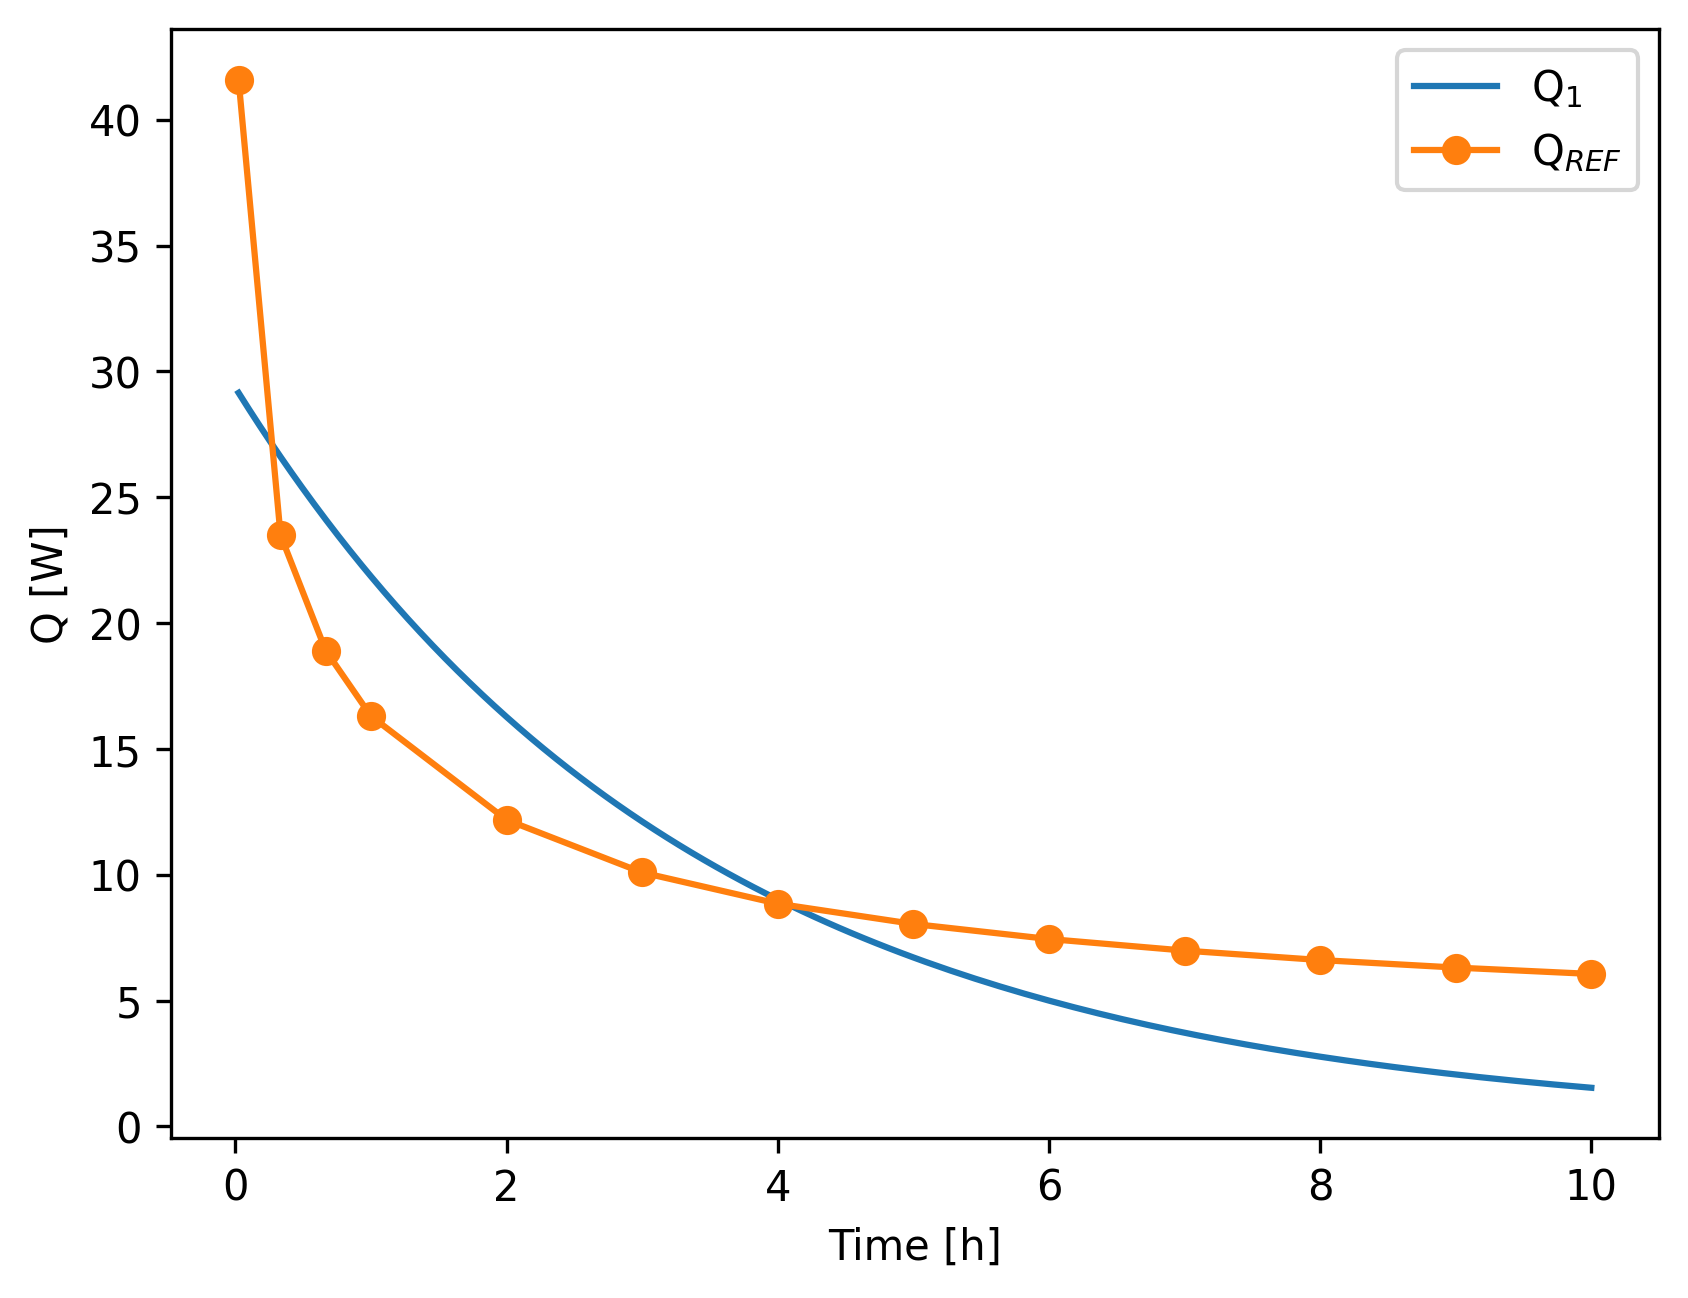
\includegraphics[width=0.45\linewidth]{figures/pure-exponential-demo}
    \hfill
    \caption{Source representation with one pure exponential decay.}
    \label{fig:one-exp}
\end{figure}

This section studies the possibility of decomposing the delayed heating over time into a linear combination of exponential decay functions
\begin{align}
Q(t) &= \mathlarger{\sum}_i^N Q_i(t) \label{eq:decomp} \\
Q_i(t) &= Q_{i, 0} e^{(-t/\tau_i)}
\end{align}
where $Q_{i,0}$ is the initial value, $\tau$ is the decay constant, and $N$ the number of terms.
The result from some investigation in available algorithms to solve this problem highlights the Prony analysis developed in 1795.
More recent work on practical implementations of the method \cite{expsum1}\cite{expsum2} intended to solve the method's drawbacks.
Since the original method finds the exponential coefficients using the roots of a polynomial, the coefficients can be positive, negative, or complex-valued.
The newer methods still have some drawbacks, and some results show estimation errors in the order of 50 \% \cite{expsum0}.

For this reason, this work uses a slightly different approach where a function of variable number of terms is chosen and their coefficients are fitted to the delayed heating.
Then, by looking at the L$_2$-norm error between the reference values and the fitted functions, it is possible to determine the most appropriate number of terms.
The implementation uses the \textit{curve\_fit} function \cite{2020SciPy-NMeth}.

To investigate this source decomposition strategy, this study uses the delayed heating over time from the demonstration problem from Section \ref{sec:demo} and the ATR experiment from Section \ref{sec:atrexp}.
Figures \ref{fig:modes-demo} and \ref{fig:modes-atr} display the results for the demonstration case and the ATR experiment.
Figures \ref{fig:modes-demo-a} and \ref{fig:modes-atr-a} show the approximation to the original data using an increasing number of terms.
A function using three terms is good enough to represent the delayed heating over time.
Figures \ref{fig:modes-demo-b} and \ref{fig:modes-atr-b} confirm this by displaying the $L_2$-norm error for the cases with an increasing number of terms.
For the ATR case, the $L_2$-norm error for the 3-term and 4-term functions are equal.
The \textit{curve\_fit} function fails to resolve the coefficients of the 4th term because more delayed heating data points are required.

Figures \ref{fig:modes-demo-c} and \ref{fig:modes-atr-c} display the individual terms of the approximated delayed heating.
The delayed heating of the demonstration case is decomposed into the following functions
\begin{align}
Q_1(t)[W] &= 14.96 e^{(-t / 1.296 h)}  \\
Q_2(t)[W] &=  9.97 e^{(-t / 19.586 h)}  \\
Q_3(t)[W] &= 19.89 e^{(-t / 0.150 h)}
\end{align}
And the delayed heating of the ATR experiment is decomposed into the following functions
% atr-1
\begin{align}
Q_1(t)[W] &= 550.7 e^{(-t / 0.019 h)}  \\
Q_2(t)[W] &= 117.0 e^{(-t / 19.078 h)}  \\
Q_3(t)[W] &= 188.4 e^{(-t / 1.057 h)}
\end{align}
% atr-2
% \begin{align}
% Q_1(t)[W] &= 553.6 e^{(-t / 0.019 h)}  \\
% Q_2(t)[W] &= 122.6 e^{(-t / 18.196 h)}  \\
% Q_3(t)[W] &= 193.8 e^{(-t / 1.013 h)}
% \end{align}

Both cases are decomposed into three exponential decay functions.
Each of the functions represents the source behavior at different time periods: short, intermediate, and long.
Both cases show a sharp decay at the beginning of the transient and a slower decay at the end.
This behavior is captured by the functions with smallest and largest decay times, respectively.

% Demonstration case
\begin{figure}[htbp!] % or H
  \centering
  \begin{subfigure}[b]{0.48\textwidth}
    \centering
    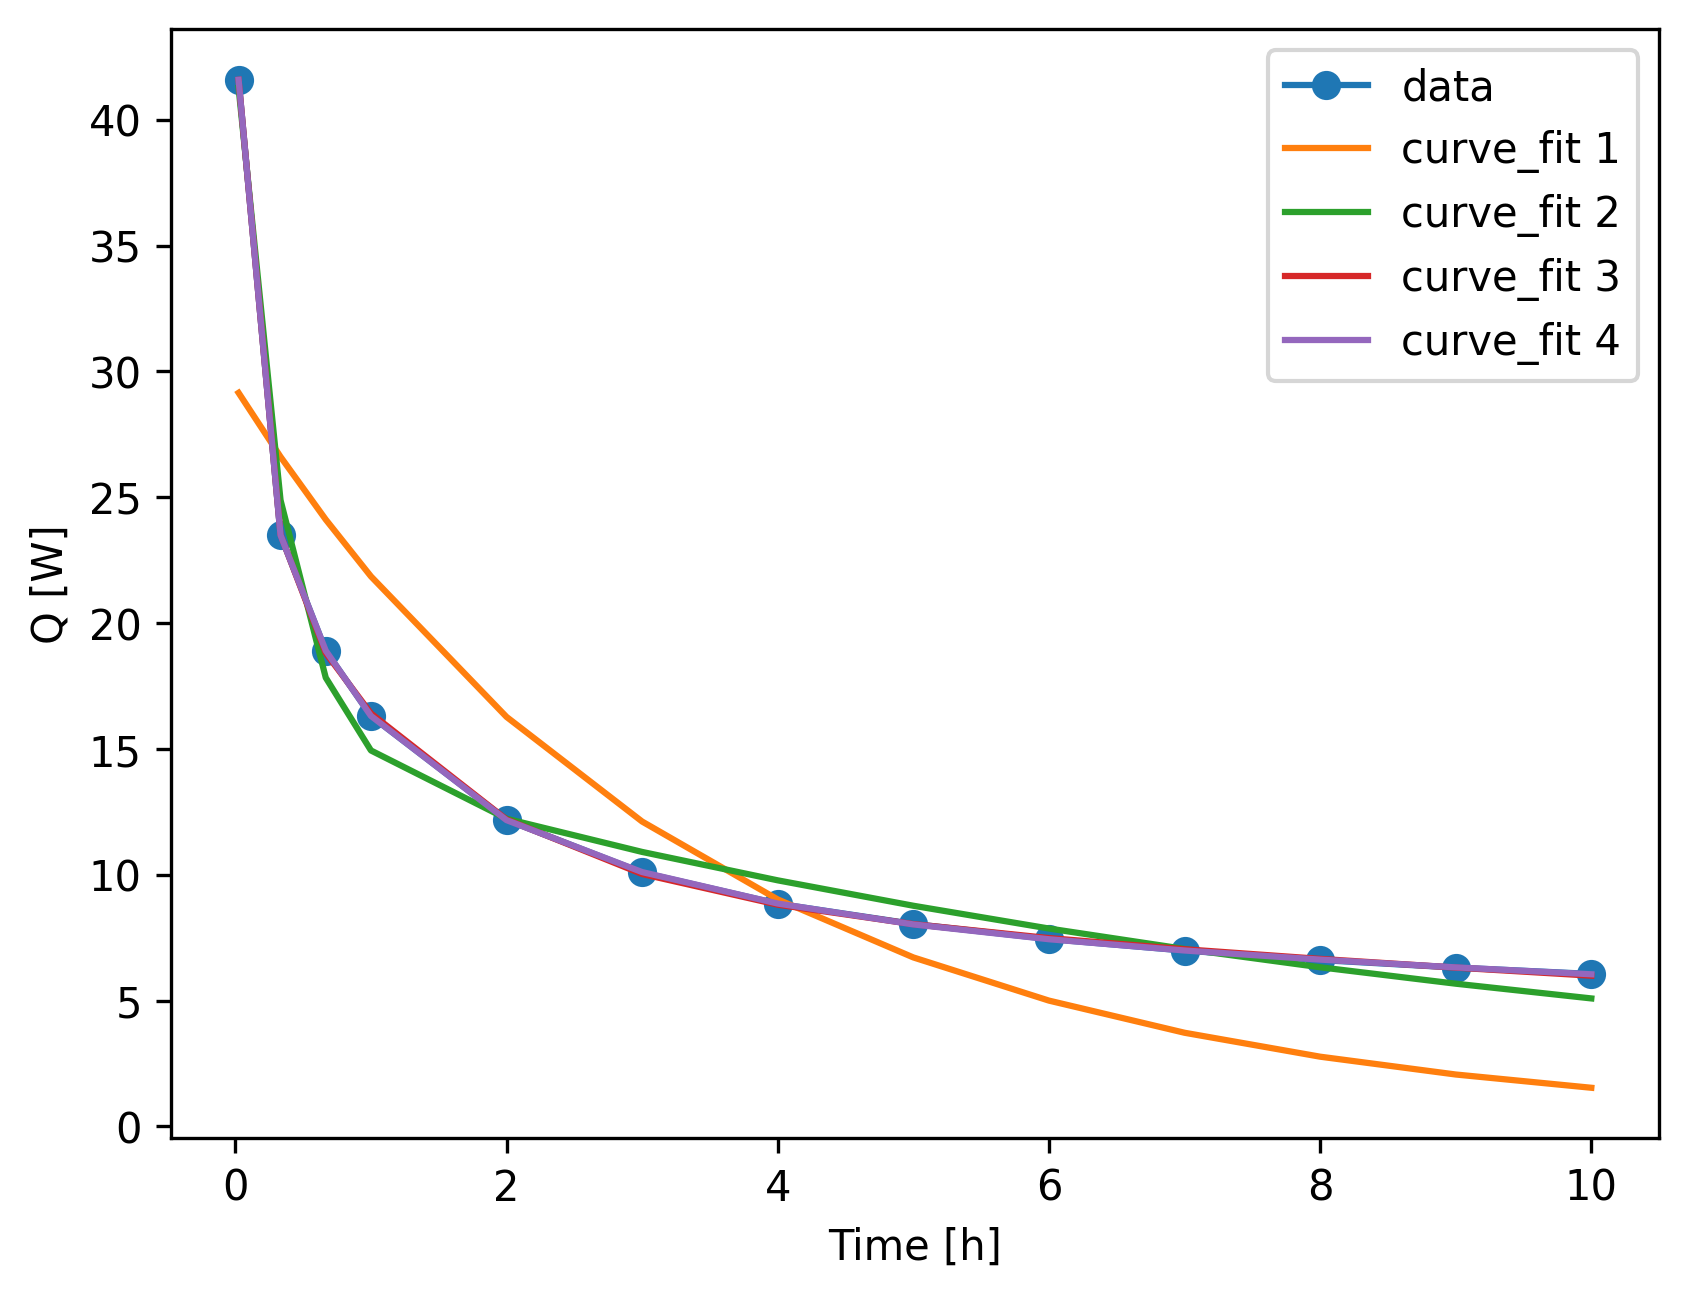
\includegraphics[width=0.98\textwidth]{figures/demo-ft}
    \caption{Approximation to the original data for different number of terms}
    \label{fig:modes-demo-a}
  \end{subfigure}
  \hfill
  \begin{subfigure}[b]{0.48\textwidth}
    \centering
    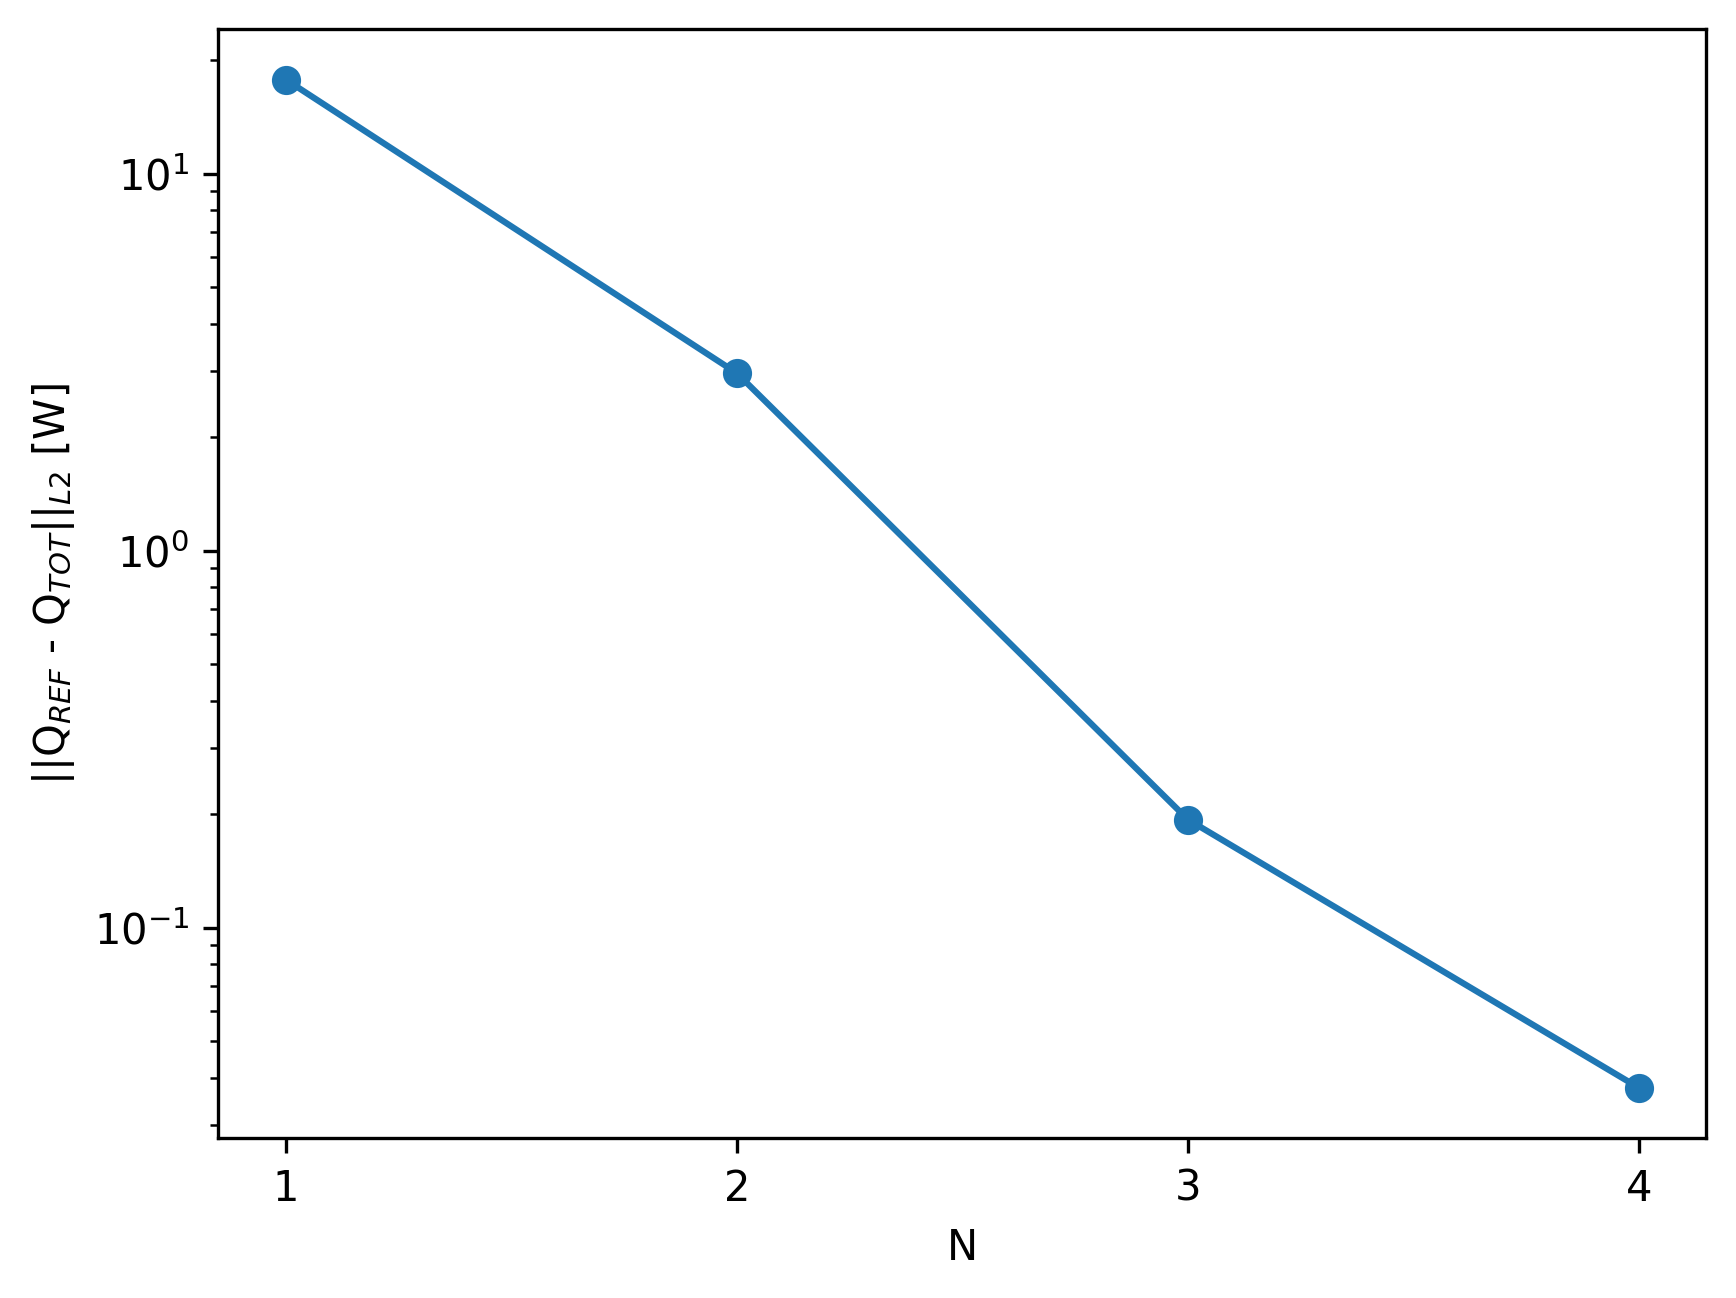
\includegraphics[width=0.98\textwidth]{figures/demo-er}
    \caption{$L_2$-norm vs. number of terms}
    \label{fig:modes-demo-b}
  \end{subfigure}
  \hfill
  \begin{subfigure}[b]{0.48\textwidth}
    \centering
    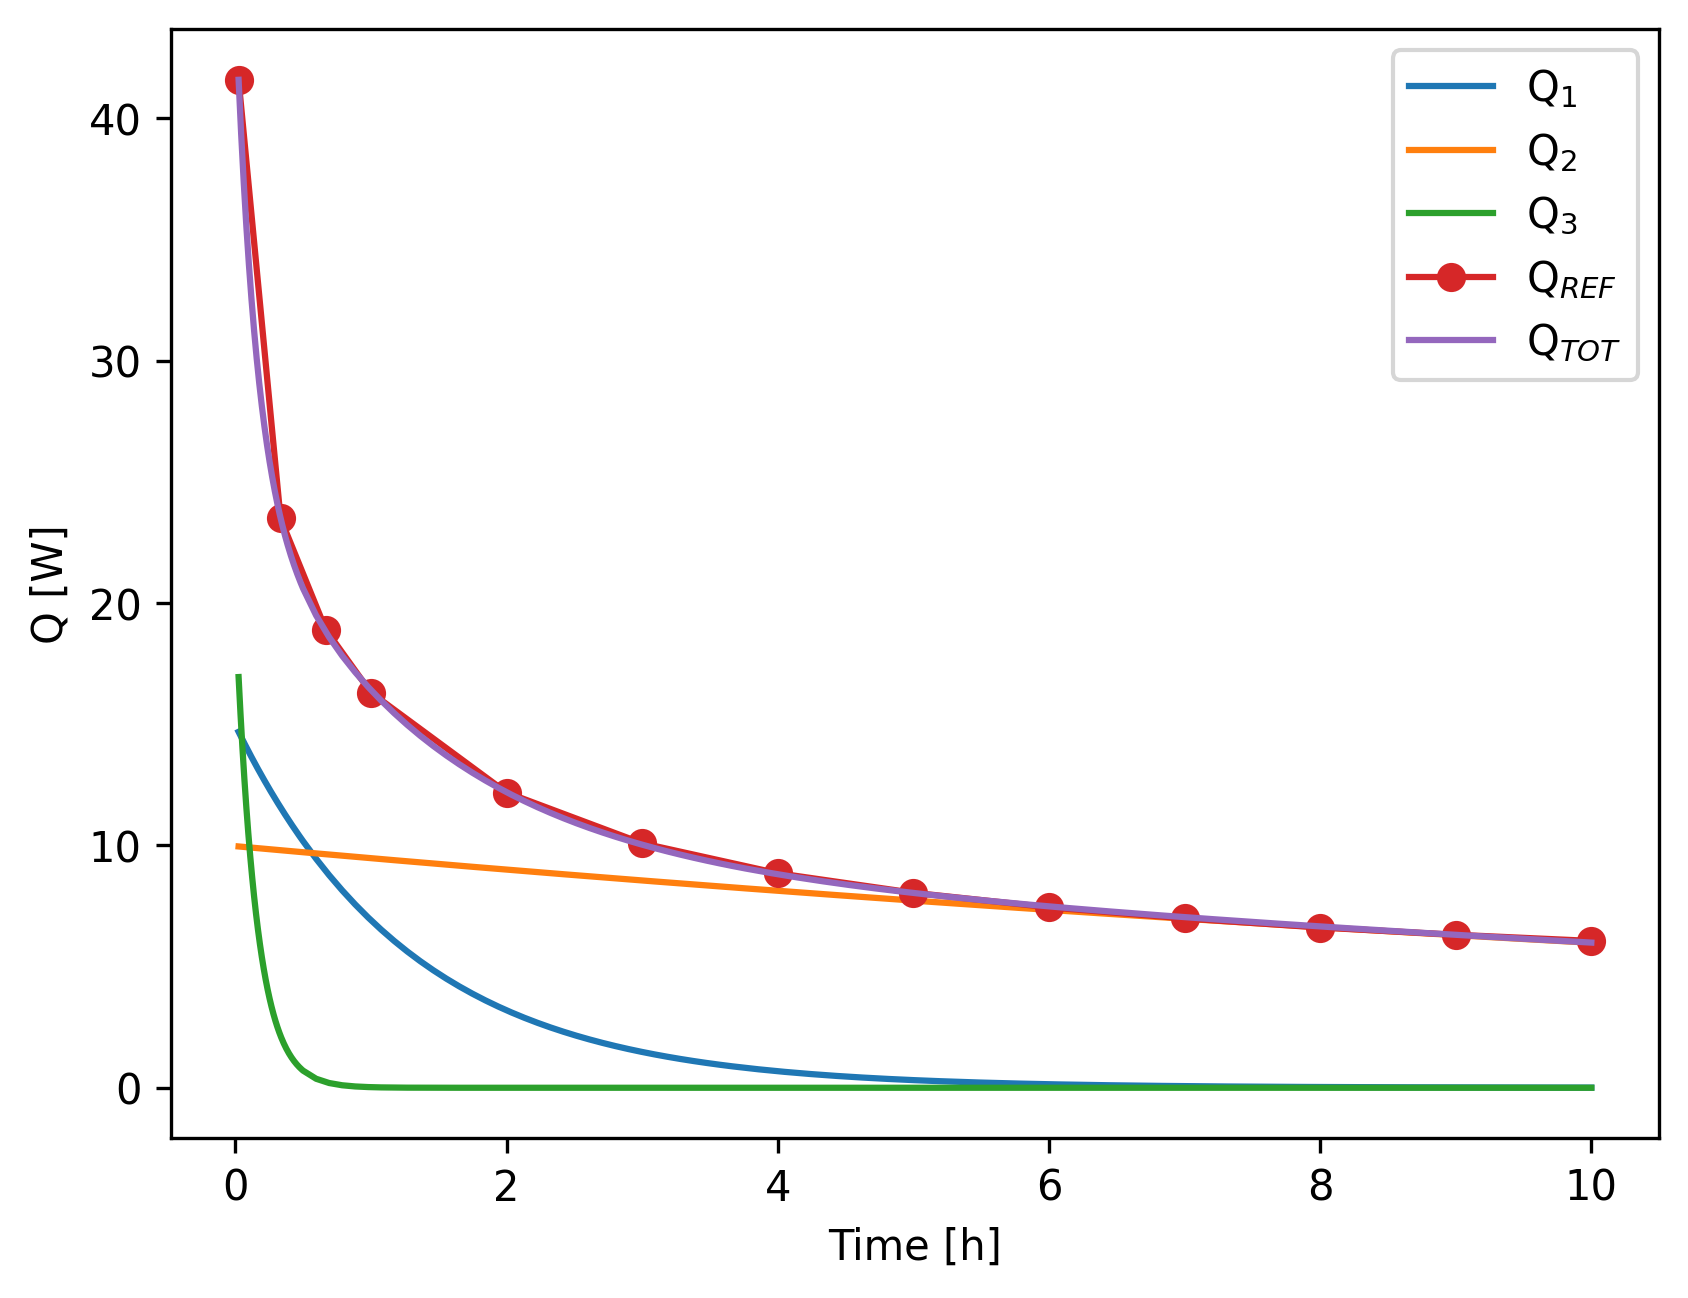
\includegraphics[width=0.98\textwidth]{figures/demo-deco-2}
    \caption{Continuous representation of the original data using three terms}
    \label{fig:modes-demo-c}
  \end{subfigure}
  \caption{Delayed heating over time approximated by a linear combination of exponential decay functions for demonstration problem of Section \ref{sec:demo}.}
  \label{fig:modes-demo}
\end{figure}
% Q1 = 7.937e+05 W/m3 exp(-t / 4664.815 s), 1.496e+01 W, 1.296 h
% Q2 = 5.289e+05 W/m3 exp(-t / 70508.195 s), 9.969e+00 W, 19.586 h
% Q3 = 1.055e+06 W/m3 exp(-t / 538.910 s), 1.989e+01 W, 0.150 h

% ATR example
\begin{figure}[htbp!] % or H
  \centering
  \begin{subfigure}[b]{0.48\textwidth}
    \centering
    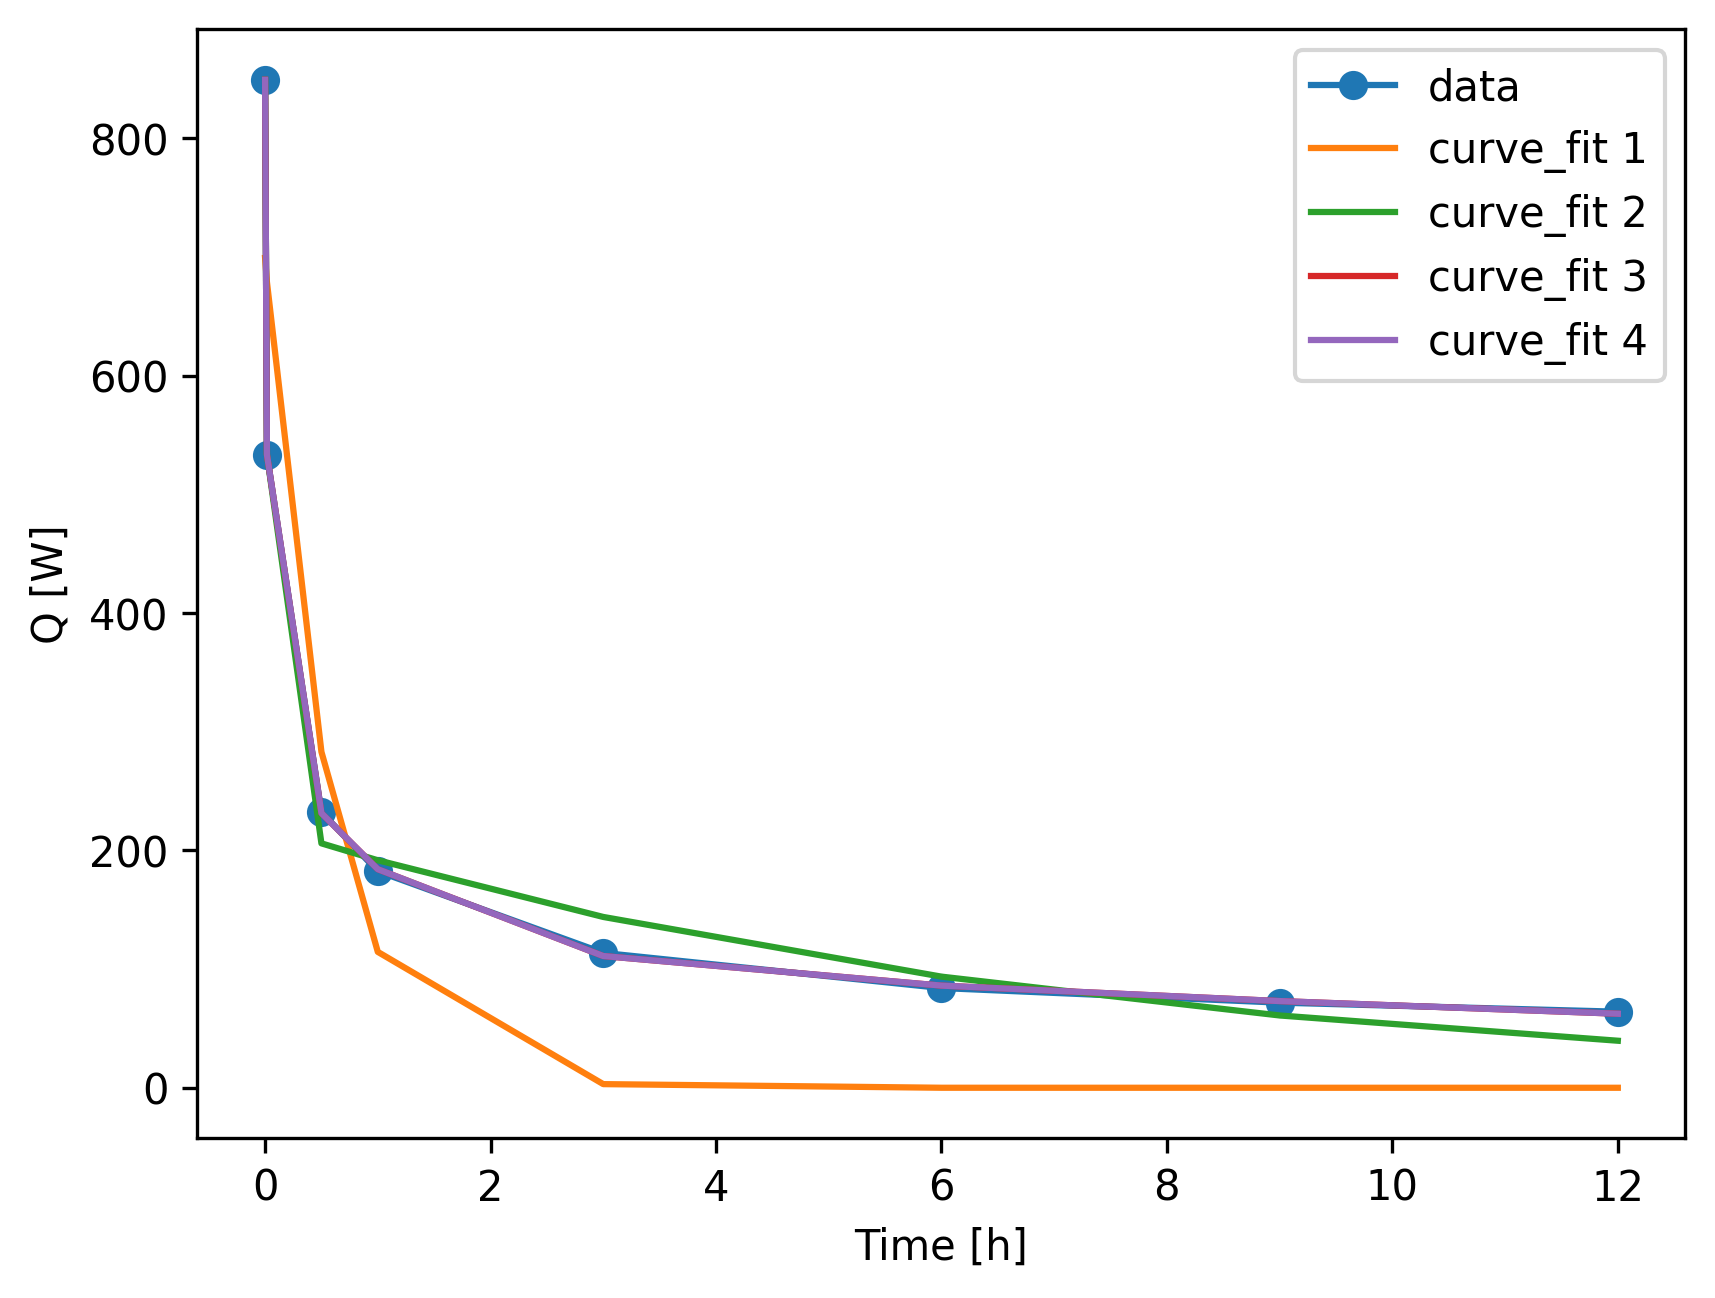
\includegraphics[width=0.98\textwidth]{figures/atr-13-ft}
    \caption{Approximation to the original data for different number of terms}
    \label{fig:modes-atr-a}
  \end{subfigure}
  \hfill
  \begin{subfigure}[b]{0.48\textwidth}
    \centering
    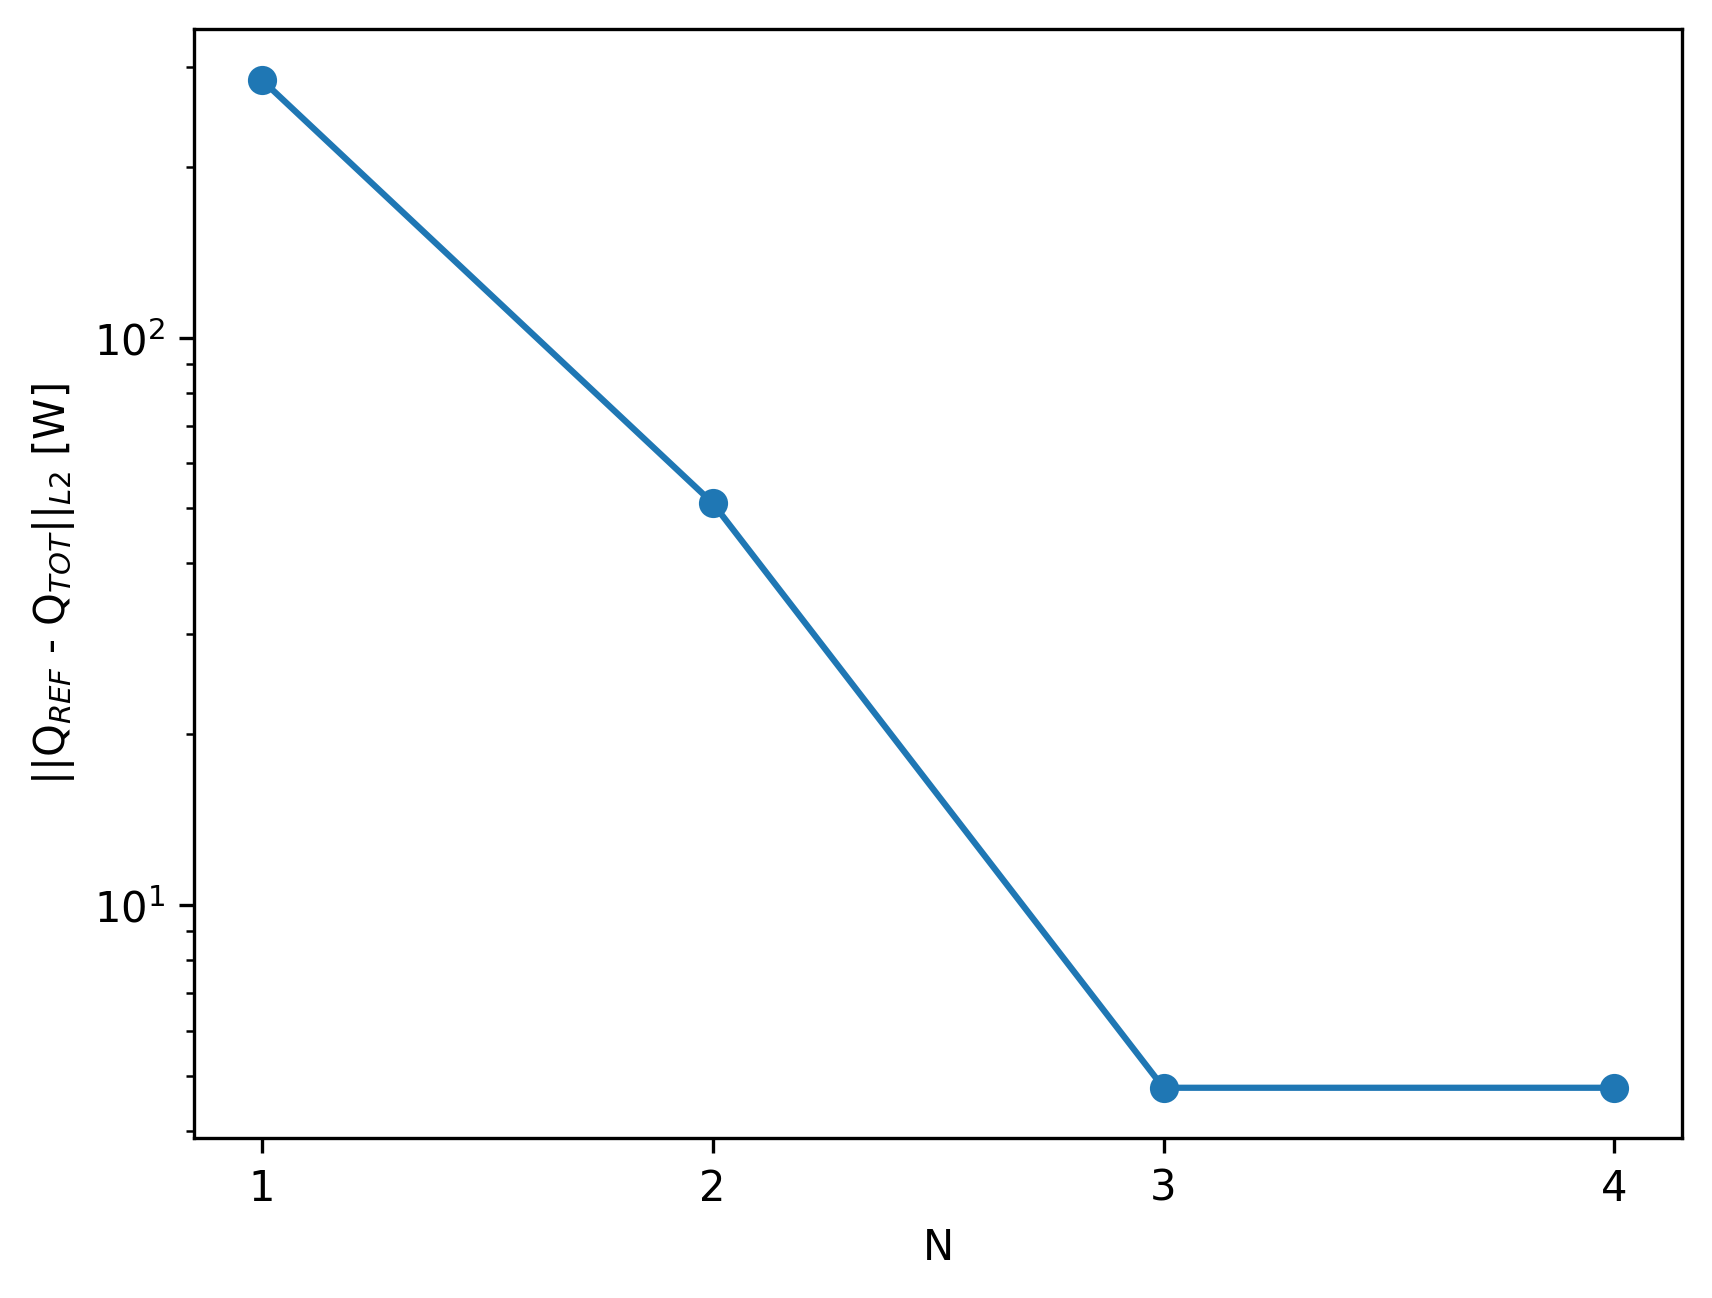
\includegraphics[width=0.98\textwidth]{figures/atr-13-er}
    \caption{$L_2$-norm vs. number of terms}
    \label{fig:modes-atr-b}
  \end{subfigure}
  \hfill
  \begin{subfigure}[b]{0.48\textwidth}
    \centering
    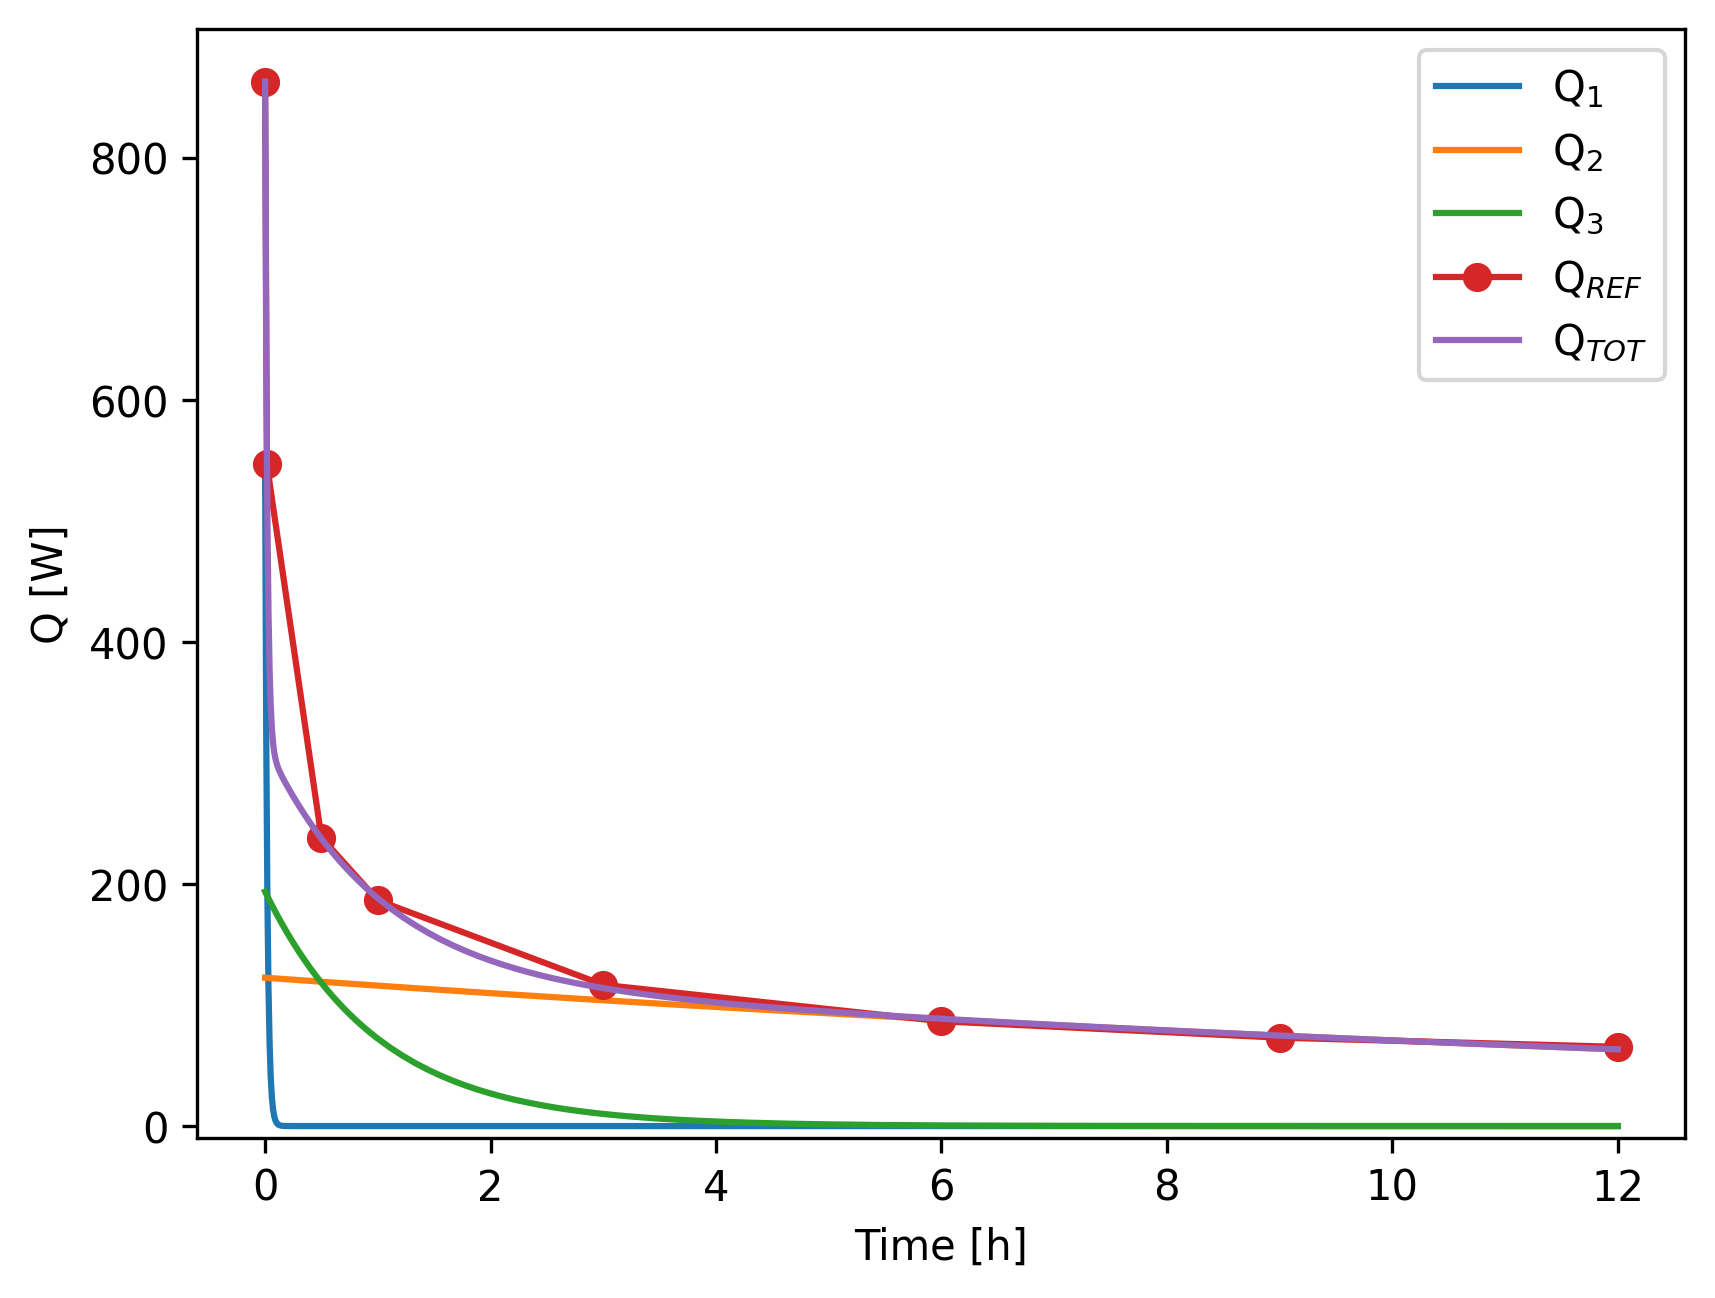
\includegraphics[width=0.98\textwidth]{figures/atr-13-deco-2}
    \caption{Continuous representation of the original data using three terms}
    \label{fig:modes-atr-c}
  \end{subfigure}
  \caption{Delayed heating over time approximated by a linear combination of exponential decay functions for ATR experiment of Section \ref{sec:atrexp}.}
  \label{fig:modes-atr}
\end{figure}

% Conclusions
These results show that the delayed heating can be approximated with a linear combination of exponential decay functions.
Utilizing three terms in the linear combination has proven a good approximation for the demonstration problem and the ATR experiment.
Additionally, the main implication from these results is that the data-based models utilized in the simplified problem from Section \ref{sec:simpl-model} are not directly applicable to a real experiment without a small modification.
Previously, the data-based models of the simplified model defined five input features - i.e., $\rho$, $c_p$, $k$, $q_0$, and $\tau$.
The new models should include the exponential coefficients defining all the terms in the delayed heating decomposition: $\rho$, $c_p$, $k$, $q_{1,0}$, $q_{2,0}$, $q_{3,0}$, $\tau_1$, $\tau_2$, and $\tau_3$.


\section{ATR experiment}
\label{sec:atr}

This section studies the application of data-based modeling to a full-size experiment hosted by the ATR.
The training and testing data is the temperature evolution of the capsule during the channel draining event, and it is generated using OpenFOAM.
% fin vs unfinned
As the capsule specification for ATR is not openly available, the designs utilized in \gls*{HFIR} experiments guide the modeling assumptions.
Figure \ref{fig:hfir-rabbit} shows a typical finned rabbit design utilized in HFIR.
The term rabbit housing refers to the outer capsule, which is in direct contact with the reactor primary coolant, used to contain the sample material.

\begin{figure}[htbp!] %or H 
    \centering
    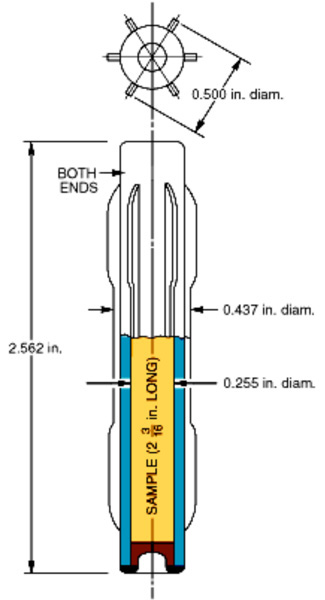
\includegraphics[width=0.30\linewidth]{figures/finned-rabbit}
    \hfill
    \caption{Typical finned capsule (also known as rabbit) design utilized in HFIR experiments. Image reproduced from \cite{hfir}.}
    \label{fig:hfir-rabbit}
\end{figure}

% \cite{hfir} Section 9.2
There are a total of six different rabbit housing designs approved for HFIR \cite{hfir}:
\begin{itemize}
  \item standard finned rabbit: this is the original design developed for use in a single tube hydraulic facility to conduct irradiations supporting isotope production.
  \item increased bore finned rabbit: similar to the standard finned rabbit with a larger inner diameter to provide larger volume for sample material.
  \item reduced bore finned rabbit: similar to standard finned rabbit with a decreased inner diameter to minimize sample temperature when irradiating small samples.
  \item un-finned rabbit: the whole concept of finned tubes is to increase the outside surface area of the tube in contact with the coolant and enhance its cooling. Un-finned rabbits allow for higher testing temperatures in the samples and are primarily used to conduct irradiations supporting material testing.
  \item un-finned selenium rabbit: similar to un-finned rabbit, with the specific use of selenium pellet irradiation.
  \item perforated rabbit: allows the reactor coolant to flow into the specimens to maintain test specimen temperature as low as possible. It is exclusively used for material irradiation testing when low testing temperatures are required.
\end{itemize}

% geometry description
This work adopts the un-finned rabbit capsule design as the problem geometry for the thermal-fluids model of the ATR experiment, as shown in Figure \ref{fig:atr-geo}.
The geometry uses a two-dimensional representation due to azimuthal symmetry, and it is represented as a wedge with a symmetric 2$^\circ$ opening with respect to the symmetry plane.
Two aspects should be mentioned about the modeling choice.
First, modeling azimuthal symmetry in OpenFOAM requires a wedge representation of the geometry as it is a \gls*{FVM} tool.
\gls*{FVM} tools require the definition of volumes in the mesh, while azimuthal symmetry is represented as a plane in \gls*{FEM} tools. 
Second, the choice of a two-dimensional representation for other rabbit designs that include fins may be inaccurate and should be investigated.

The dimensions of the geometry are based on the ATR experiment dimensions and typical dimensions of HFIR finned and un-finned rabbits.
This exercise focuses on the A1 experiment position which has a fixed 0.625'' diameter or 7.94 mm radius and sets the radius of the channel outer wall.
The gap between the capsule and channel outer walls is defined by the fin width which is 0.8 mm.
The thickness of the capsule is defined by the thickness of the increased bore finned rabbit which is 1.4 mm, and it is assumed for the capsule walls in the radial and axial direction.
Finally, the capsule length is set by the experiment position height, being 1.22 m \cite{inl_advanced_2009}.

% D_A1: 0.625" = 0.0079375 m
% Gap between capsule and channel wall: (0.5-0.437)" / 2 = 0.08 cm
% Experiment radius: 0.0071375 m
% Thickness comes from increased bore finned rabbit:
% (Outer diam: 0.437" - inner Diam: 0.324")/2 = 1.435 mm --> 0.0014 m

% Total height 1.22 m
% Capsule thickness 0.0014 m
% Experiment radius: 0.0057375 m
% Experiment height: 1.2172 m
% External channel radius: 0.0079375 m

\begin{figure}[htbp!] %or H 
    \centering
    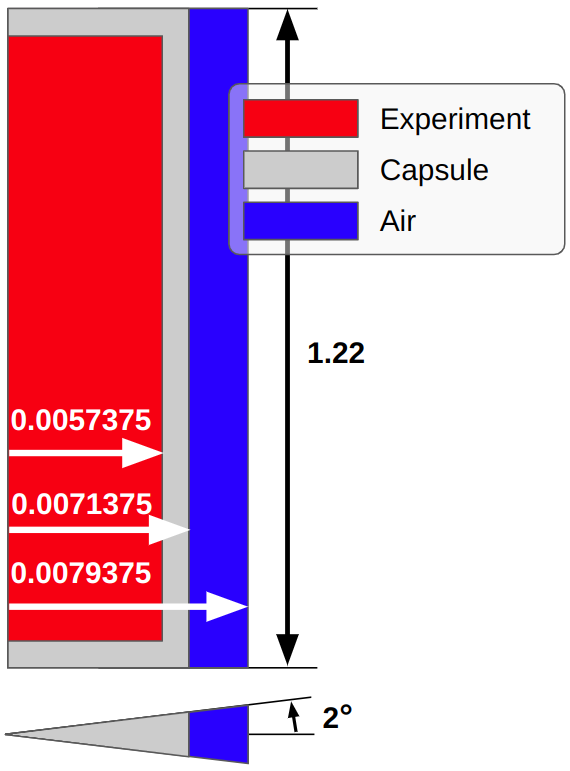
\includegraphics[width=0.40\linewidth]{figures/atr-geometry}
    \hfill
    \caption{ATR experiment geometry for the thermal-fluids model. Dimensions not at scale to better display the model regions. Dimensions expressed in $m$.}
    \label{fig:atr-geo}
\end{figure}

% Material properties
The problem defines a multi-region geometry with two solid regions: capsule and experiment, and one fluid region: air.
The capsule is made of aluminum 6061-T6 \cite{inl_advanced_2009} with the material properties specified in Table \ref{tab:al-props}.
The emissivity of the aluminum is necessary when including a thermal radiation model.
Its value is highly dependent on the material surface conditions.
For highly polished aluminum, the emissivity ranges from 0.039 to 0.057, and this work assumes an average value of 0.05.
The air material properties assume a 323 K (50 $^\circ$C) temperature and 100 kPa pressure and are shown in Table \ref{tab:al-props}.
Since the experiment material is variable, its material properties are not fixed and are not included in the table.
Appendix \ref{ap:mat_props} shows all the materials included in the model and their properties.

\begin{table}[htbp!]
  \centering
  \caption{Material properties of capsule and air.}
  \label{tab:al-props}
  \begin{tabular}{cccc}
    \toprule
      Properties     & Units     & Capsule                & Air                    \\
    \midrule
      Molecular weight & g/mol   & 27                     & 28.9                   \\
      $\rho$         & kg/m$^3$  & 2.7 $\times$ 10$^{3}$  & -                      \\
      $k$            & W/m/K     & 167                    & -                      \\
      $c_p$          & J/kg/K    & 896                    & 1000                   \\
      $\varepsilon$  & -         & 0.05                   & -                      \\
      Melting temperature     & $^\circ$C & 650                    & -                      \\
      $\mu$          & kg/m/s    & -                      & 1.8 $\times$ 10$^{-5}$ \\
      $Pr$           & -         & -                      & 0.7                    \\
    \bottomrule
  \end{tabular}
\end{table}

% mesh
% https://www.openfoam.com/documentation/guides/latest/doc/guide-bcs-constraint-wedge.html
The mesh of the model was created with GMSH v4.10.5\cite{geuzaine_gmsh_2009} and is shown in Figure \ref{fig:atr-msh}.
It was created as coarse as possible to reduce the computation expense, while still allowing for a smooth representation of the temperature in the different regions.
The two-dimensional representation of the geometry in OpenFOAM requires the boundary surfaces to straddle the symmetry plane equally with a single layer of cells in the azimuthal direction, and the points on both surfaces should appear collocated when viewed in the symmetry plane normal direction.

\begin{figure}[htbp!] %or H 
  \centering
  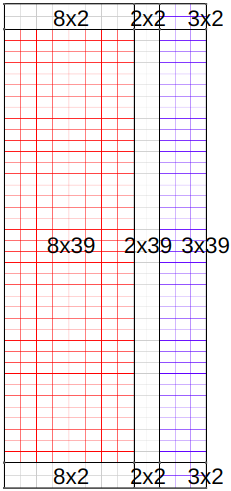
\includegraphics[width=0.25\linewidth]{figures/atr-mesh}
  \hfill
  \caption{Mesh of the ATR experiment geometry for the thermal-fluids model.}
  \label{fig:atr-msh}
\end{figure}

% laminar vs turbulence
% g = 9.8
% beta = 1/T = 1/323
% Tinf = 323
% S = 0.0079375 - (0.0057375+0.0014) = 0.0008 m
% nu = 1.48e-5
% alpha = nu / (Pr = 0.7) = 2.1143e-5
% Ra_S(T=330 K) = 0.35
% Ra_S(T=2000 K) = 83.25
This model assumes a laminar flow for solving the equations of motion and temperature of the air.
The following correlation defines the transition to the turbulence regime for a vertical channel with natural circulation \cite{incropera_fundamentals_2006}
\begin{align}
Ra_S &= \frac{g \beta \Delta T S^3}{\alpha \nu}
\end{align}
where $Ra_{S}$ is the Rayleigh number, $g$ is the acceleration due to gravity, $\beta$ is the thermal expansion coefficient of air, $\Delta T$ is the difference between the surface temperature and air inlet temperature, $S$ is the channel thickness, $\alpha$ is the thermal diffusivity of air, and $\nu$ is the kinematic viscosity of air.
Assuming an air reference pressure and temperature of 100 kPa and 323 K (50 $^\circ$C), $\beta$, $\nu$ and $\alpha$ take the values 0.003096 1/K, 1.48$\times 10^{-5}$, and 2.114 $\times 10^{-5}$.
Assuming a capsule wall temperature of 2000 K, the $Ra_S$ is 83.
With a transition to turbulent occurring $Ra$ equal to 10$^9$, and a capsule melting temperature of 923 K, the flow in the channel remains laminar.
As discussed in Section \ref{sec:simpl-model}, the addition of a thermal radiation model is necessary.
The model of the ATR experiment includes the thermal radiation model P1 already available in OpenFOAM.

% boundary conditions
% https://www.openfoam.com/documentation/guides/latest/doc/guide-bcs-derived-outlet.html
% Discussion on p_rgh: https://www.cfd-online.com/Forums/openfoam-solving/80454-p_rgh-1-7-a.html
% Flux: phi: \rho \vec{u} \cdot \vec{A}
% pp = p0 - \frac{1}{2} |u|^2
% pp: boundary pressure
% p0: total pressure
% 1/2 |u|^2: dynamic pressure
% p0 is specified at 100 kPa
% Inlet: totalPressure w/ pressureInletOutletVelocity: https://www.cfd-online.com/Forums/openfoam-solving/222974-about-totalpressure-bc.html
The boundary conditions defining the problem are specified in Figure \ref{fig:atr-bcs}.
The two-dimensional representation with azimuthal symmetry in OpenFOAM uses the \textit{wedge} boundary condition in the surfaces on each side of the wedge.
This boundary condition applies to all the regions in the geometry.
The top and bottom surfaces of the capsule are insulated, which is defined in OpenFOAM with the \textit{zeroGradient} boundary condition.
In the fluid, OpenFOAM requires boundary conditions for the temperature $T$, velocity $U$, and incident radiation field $G$.
Additionally, OpenFOAM does not solve for the static pressure directly but solves for
\begin{align}
p\_rgh &= p - \rho g h
\end{align}
where $p$ is the static pressure and $\rho g h$ is the hydrostatic pressure.
The temperature in the channel wall is assumed to be fixed at 323 K (50 $^\circ$C), and it is defined with the \textit{fixedValue} boundary condition.
The channel and capsule walls consider a \textit{noSlip} boundary condition that sets the velocity equal to zero.
The $p\_rgh$ in the channel and capsule walls takes the \textit{fixedFluxPressure} boundary condition, which sets the pressure gradient to a provided value such that the flux on the boundary is that specified by the velocity boundary condition.
The temperature at the inlet and outlet uses the \textit{InletOutlet} boundary condition, which applies a zero gradient boundary condition to the outflow and fixes the temperature of the reverse flow (fixed at 323 K).
The inlet velocity uses the \textit{pressureInletOutletVelocity} boundary condition, which assigns a zero gradient boundary condition to the outflow and assigns a velocity based on the flux in the boundary-normal direction to the inflow.
The outlet velocity uses the \textit{InletOutlet} boundary condition, and it applies a fixed zero velocity for the reverse flow.
The $p\_rgh$ uses the \textit{totalPressure} and \textit{fixedValue} boundary conditions for the inlet and outlet, respectively.
% OF documentation for the subsonic compressible, even this is not technically compressible
The \textit{totalPressure} imposes a value of 100 kPa for the total pressure $p0$, and the value for $p\_rgh$ is calculated as $p0 - \frac{\rho \|U\|^2}{2}$.
The outlet $p\_rgh$ is fixed at 100 kPa.
All fluid boundaries assume the \textit{MarshakRadiation} boundary condition for the incident radiation field $G$.
The initial condition is room temperature (323 K) for the whole geometry.

\begin{figure}[htbp!] %or H 
  \centering
  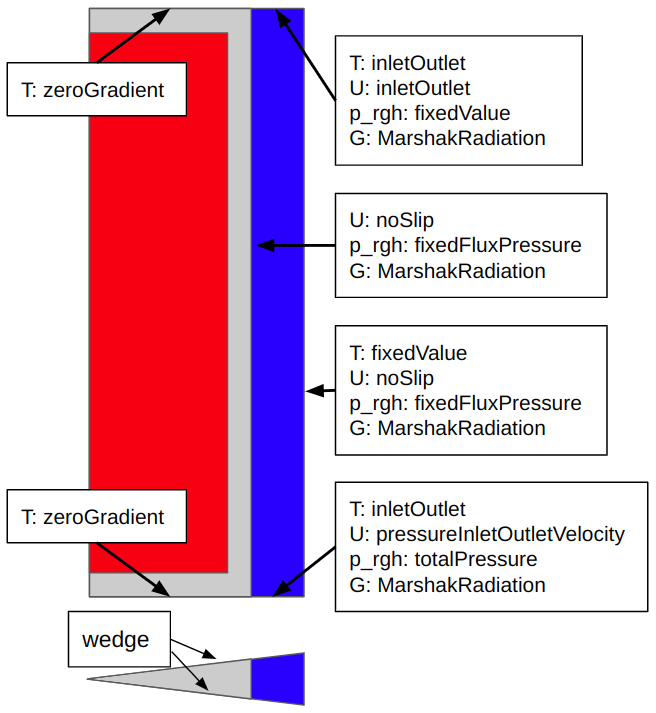
\includegraphics[width=0.45\linewidth]{figures/atr-bcs}
  \hfill
  \caption{Boundary conditions applied to the ATR experiment model in OpenFOAM.}
  \label{fig:atr-bcs}
\end{figure}

% Source
The model considers that the experiment produces volumetric heat defined by the linear combination of three exponential decay functions
\begin{align}
q'''(t) &= q_{1, 0} e^{(-t/\tau_1)} + q_{2, 0} e^{(-t/\tau_2)} + q_{3, 0} e^{(-t/\tau_3)}.
\end{align}
The source is defined in OpenFOAM using the \textit{fvOptions} file and a \textit{scalarCodedSource} object.
This model neglects the heat production ($q''' = 0$) in the capsule to simplify the analysis.
This assumption is justified by the fact that the volume of the experiment is considerably larger than the capsule's.

% Serial vs Parallel runs
% https://www.openfoam.com/documentation/user-guide/3-running-applications/3.2-running-applications-in-parallel
As mentioned earlier, OpenFOAM supports the parallelization of the simulation via domain decomposition, wherein the mesh and associated fields are separated into pieces and allocated to separate processors for solution.
The parallelization involves: decomposition of mesh and fields (\textit{decomposePar} utility), running the application in parallel, and re-composition of the fields (\textit{reconstructPar} utility).
This work uses the \textit{scotch} method for the domain decomposition, which requires no geometric input from the user and attempts to minimize the number of boundaries.

To determine the best mesh discretization number of processors pair, Table \ref{tab:serial-parallel} shows the execution time for simulations running up to 100 second-simulation time with an increasing number of processors and four different meshes with increasing number of cells, which are labelled A through D.
For all the meshes, the execution time decreases for an increasing number of processors, up to eight processors.
After this number, the execution time increases.
For a small number of cells, the communication between processors may dominate the computations, which causes the execution time to increase.
Based on these results, the simulations running in parallel use the coarser mesh and eight processors.
However, the simulation with eight processors is only 3 times faster than the serial simulation, which means that in cases where the number of processors is limited, it is preferable to run eight simulations in serial simultaneously than eight simulations in parallel subsequently.
The parallel runs are reserved for \gls*{HPC} machines where the job scheduling is not based on the number of processors per node but the allocated number of nodes.

\begin{table}[htbp!]
  \centering
  \caption{Execution time in minutes for simulations with an increasing number of processors and four different meshes (labelled A through D) with increasing number of cells.}
  \label{tab:serial-parallel}
\begin{tabular}{c|ccccc}
 \toprule
    & \multicolumn{5}{c}{Number of processors}       \\
 \midrule
  mesh label  & 1      & 4      & 8      & 12    & 16     \\
 \midrule
  A & 26.53  & 12.45  &  9.41  &  9.73 &  9.98  \\
  B & 18.88  & 16.03  & 11.38  &  -    & 12.19  \\
  C & 37.74  & 25.22  & 18.21  &  -    & 18.41  \\
  D & 83.14  & 42.34  & 33.05  &  -    & 38.69  \\
 \bottomrule
\end{tabular}
\end{table}


\subsection{Results}

% Results from two example cases:
This section shows the results for two complete cases: first, for an experiment of aluminum, and second, for an experiment of $U_3Si_2/Al$ with a 20\% enrichment.
Figure \ref{fig:modes-atr-1b} shows the delayed heating in the experiment of aluminum.
The volumetric heat can be expressed as
% atr-1
\begin{align}
q'''(t) [W/m^3] &= 1.954 \times 10^6 e^{(-t/68.649 s)} + 4.150 \times 10^5 e^{(-t/68680.862 s)} + 6.682 \times 10^5 e^{(-t/3803.589 s)}.
\end{align}
% atr-2
% \begin{align}
% q'''(t) [W/m^3] &= 1.964 \times 10^6 e^{(-t/69.081 s)} + 4.348 \times 10^5 e^{(-t/65505.079 s)} + 6.874 \times 10^5 e^{(-t/3647.724 s)}.
% \end{align}


\begin{figure}[htbp!] %or H 
    \centering
    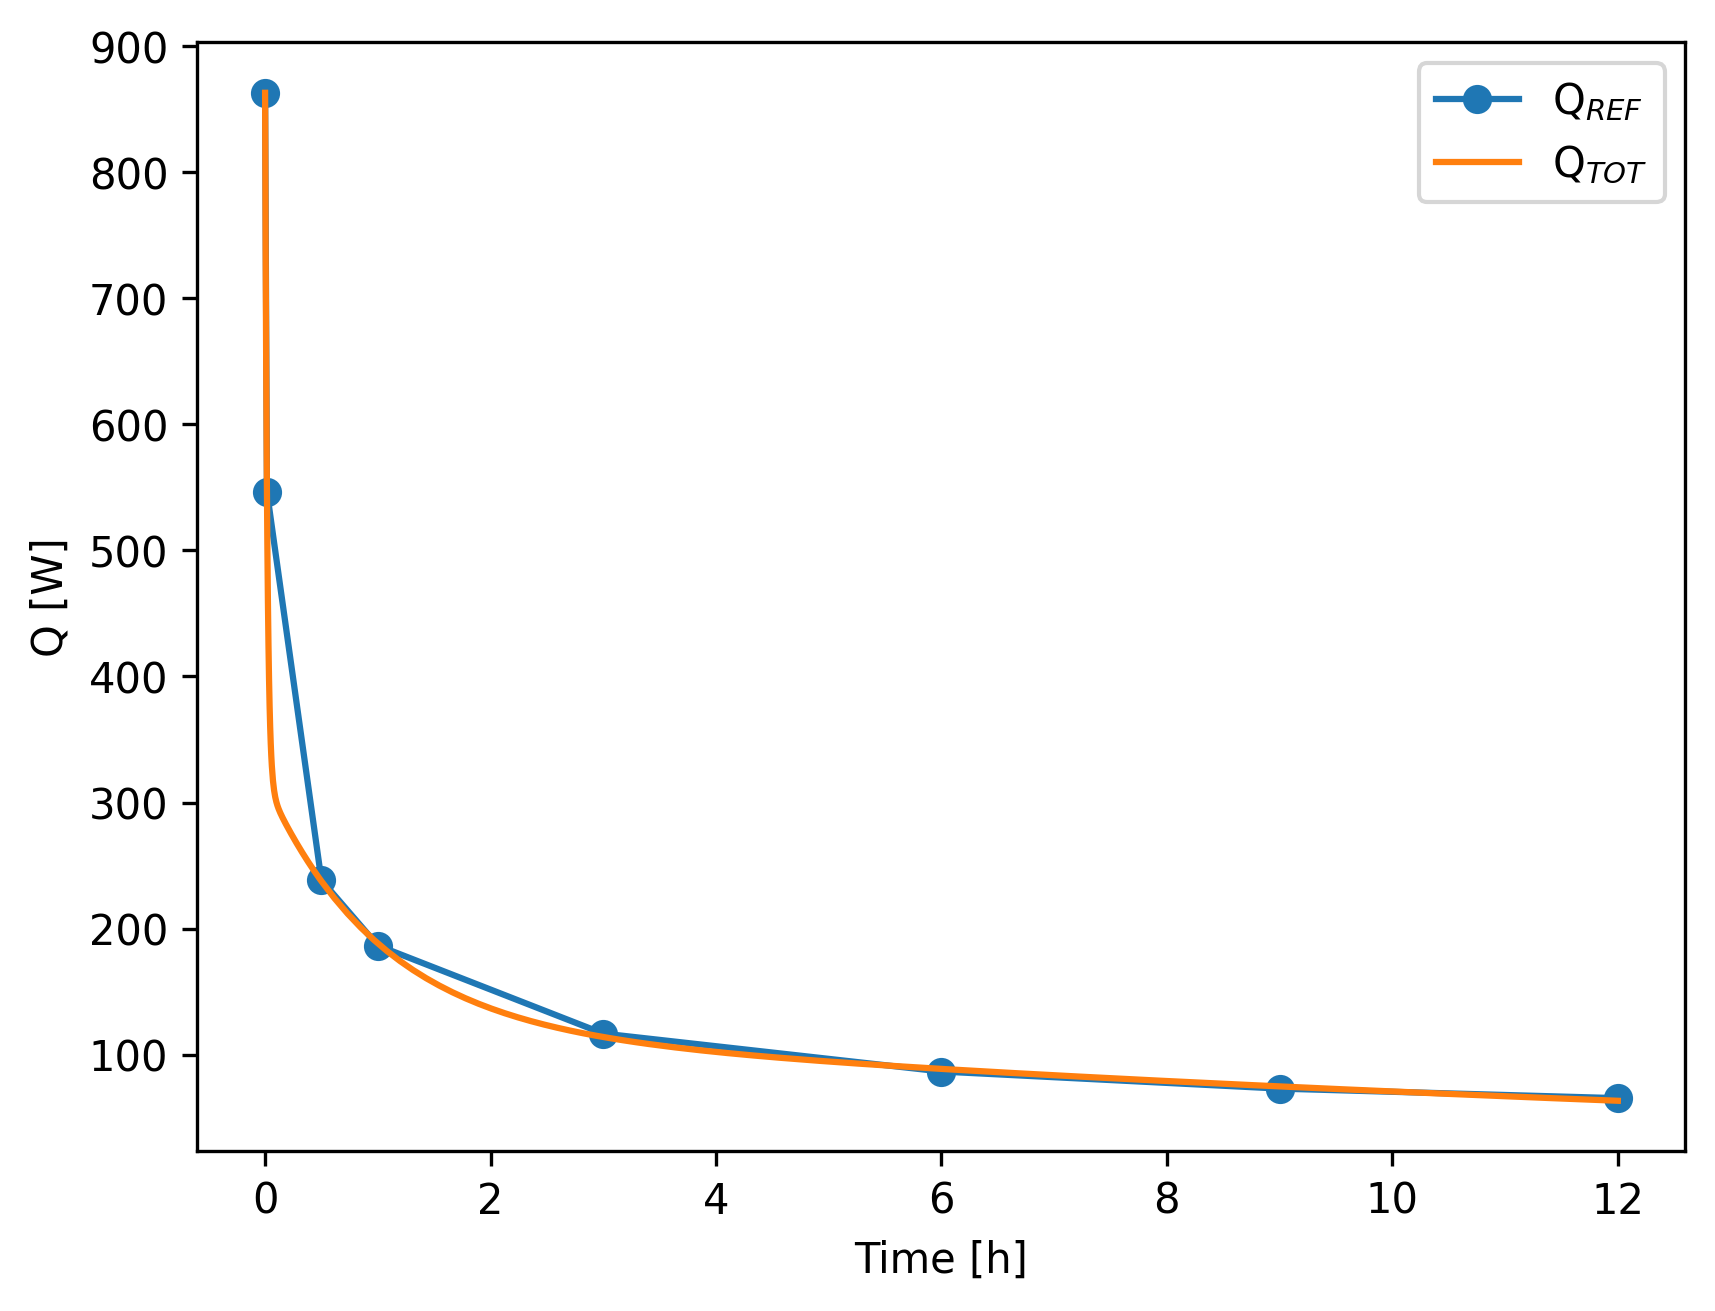
\includegraphics[width=0.45\linewidth]{figures/atr-13-deco-1}
    \hfill
    \caption{Delayed heating over time for ATR experiment of aluminum.}
    \label{fig:modes-atr-1b}
\end{figure}

The material properties of aluminum can be found in Table \ref{tab:al-props}.
Figure \ref{fig:atr-al} shows the evolution of the highest temperature in the capsule for the experiment of aluminum.
The capsule reaches the maximum temperature of 388.9 K at 580 seconds, and it is located in the capsule's inner wall at the middle of the total height.
The temperature exhibits quick and slow responses corresponding to the smallest and largest decay times of the volumetric heat.
Hence, the temperature increases rapidly from the initial condition, and after reaching the maximum, it decays slowly.
% The simulations used an adaptive time stepper between 8$\times$10$^{-4}$ and 2$\times$10$^{-3}$ s, and the total serial execution time was 1 hr 48 min.

\begin{figure}[htbp!] %or H 
    \centering
    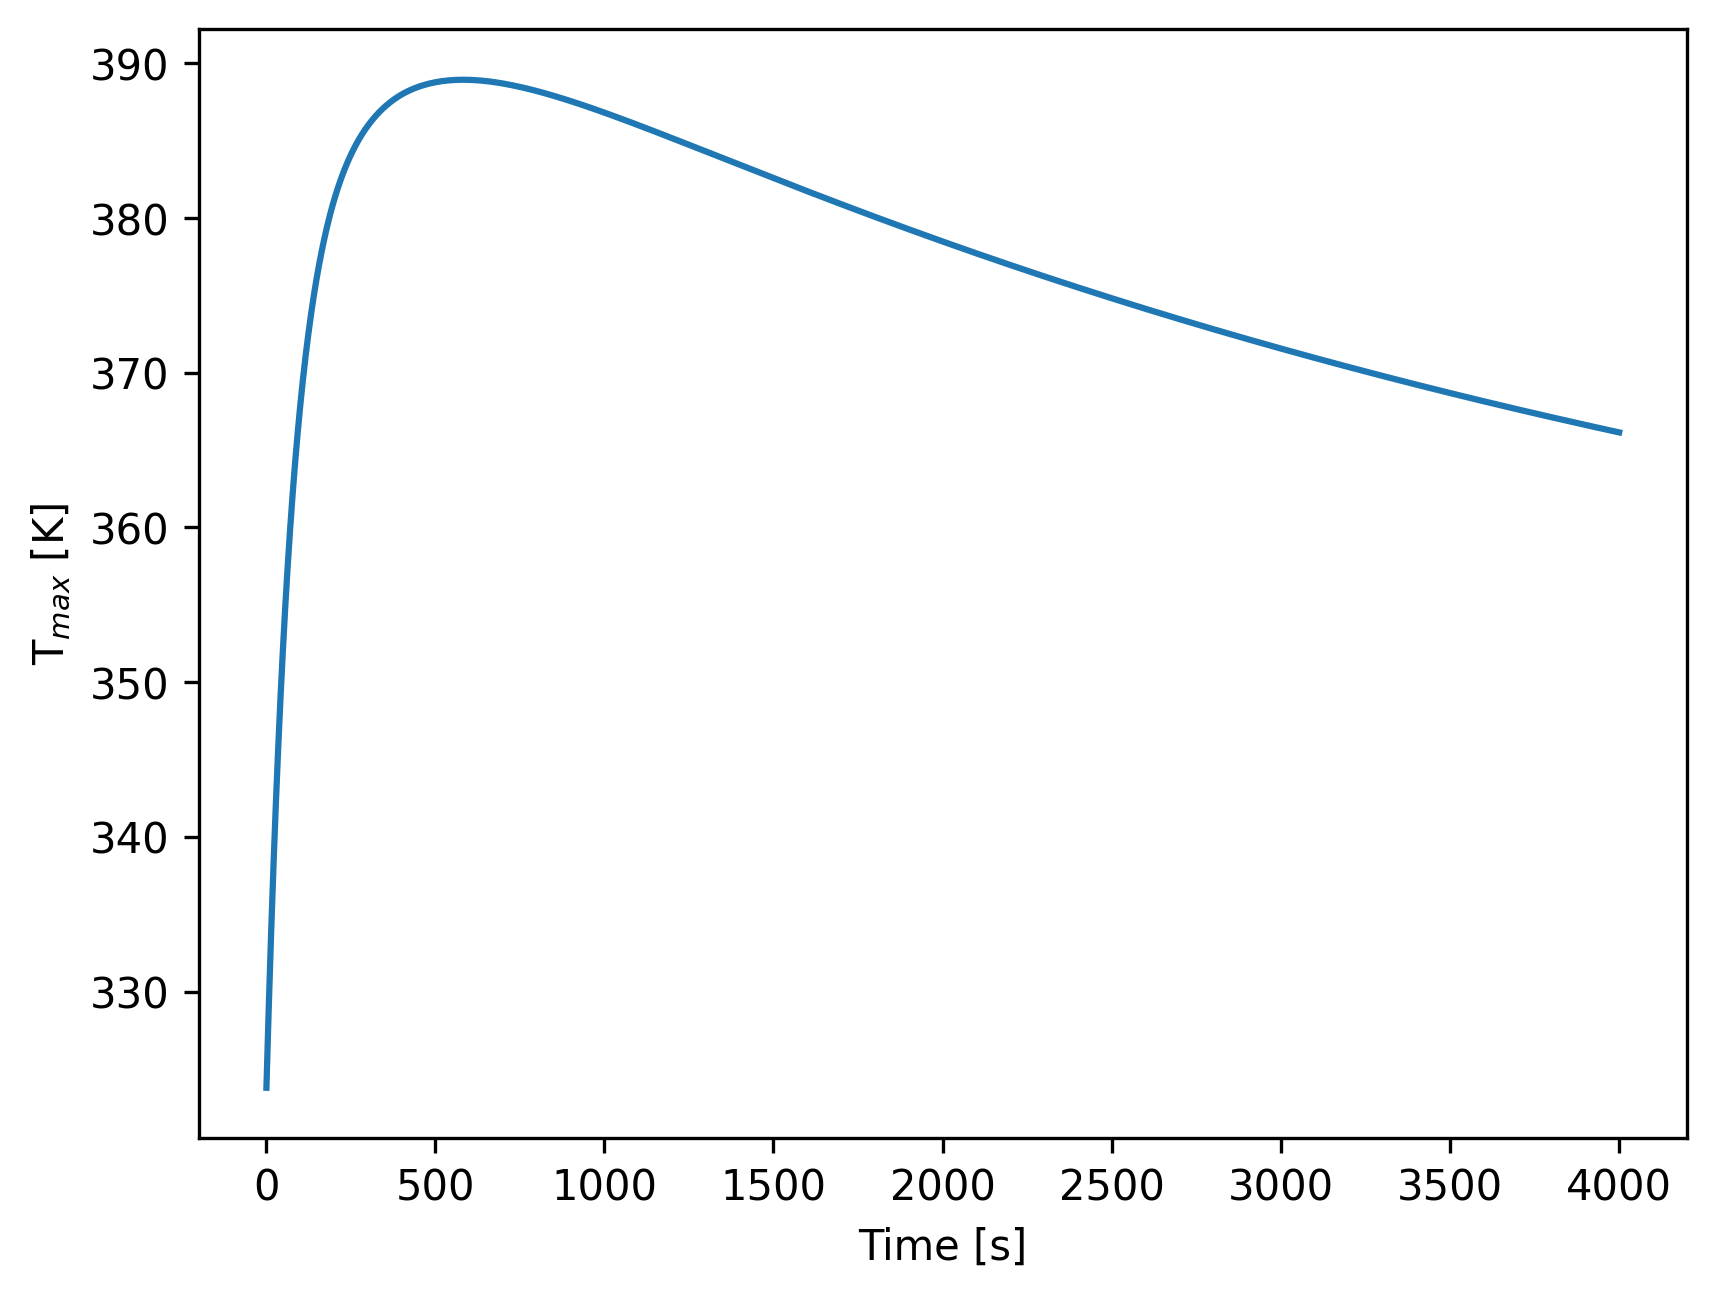
\includegraphics[width=0.45\linewidth]{figures/atr-Al}
    \hfill
    \caption{Time evolution of the highest temperature in the capsule for ATR experiment of aluminum.}
    \label{fig:atr-al}
\end{figure}

Figure \ref{fig:modes-atr-2} shows the delayed heating in the experiment of $U_3Si_2/Al$.
The volumetric heat can be expressed as
\begin{align}
q'''(t) [W/m^3] &= 6.491 \times 10^6 e^{(-t/65308.004 s)} + 2.935 \times 10^7 e^{(-t/52.145 s)} + 8.485 \times 10^6 e^{(-t/3110.743 s)}.
\end{align}

\begin{figure}[htbp!] %or H 
    \centering
    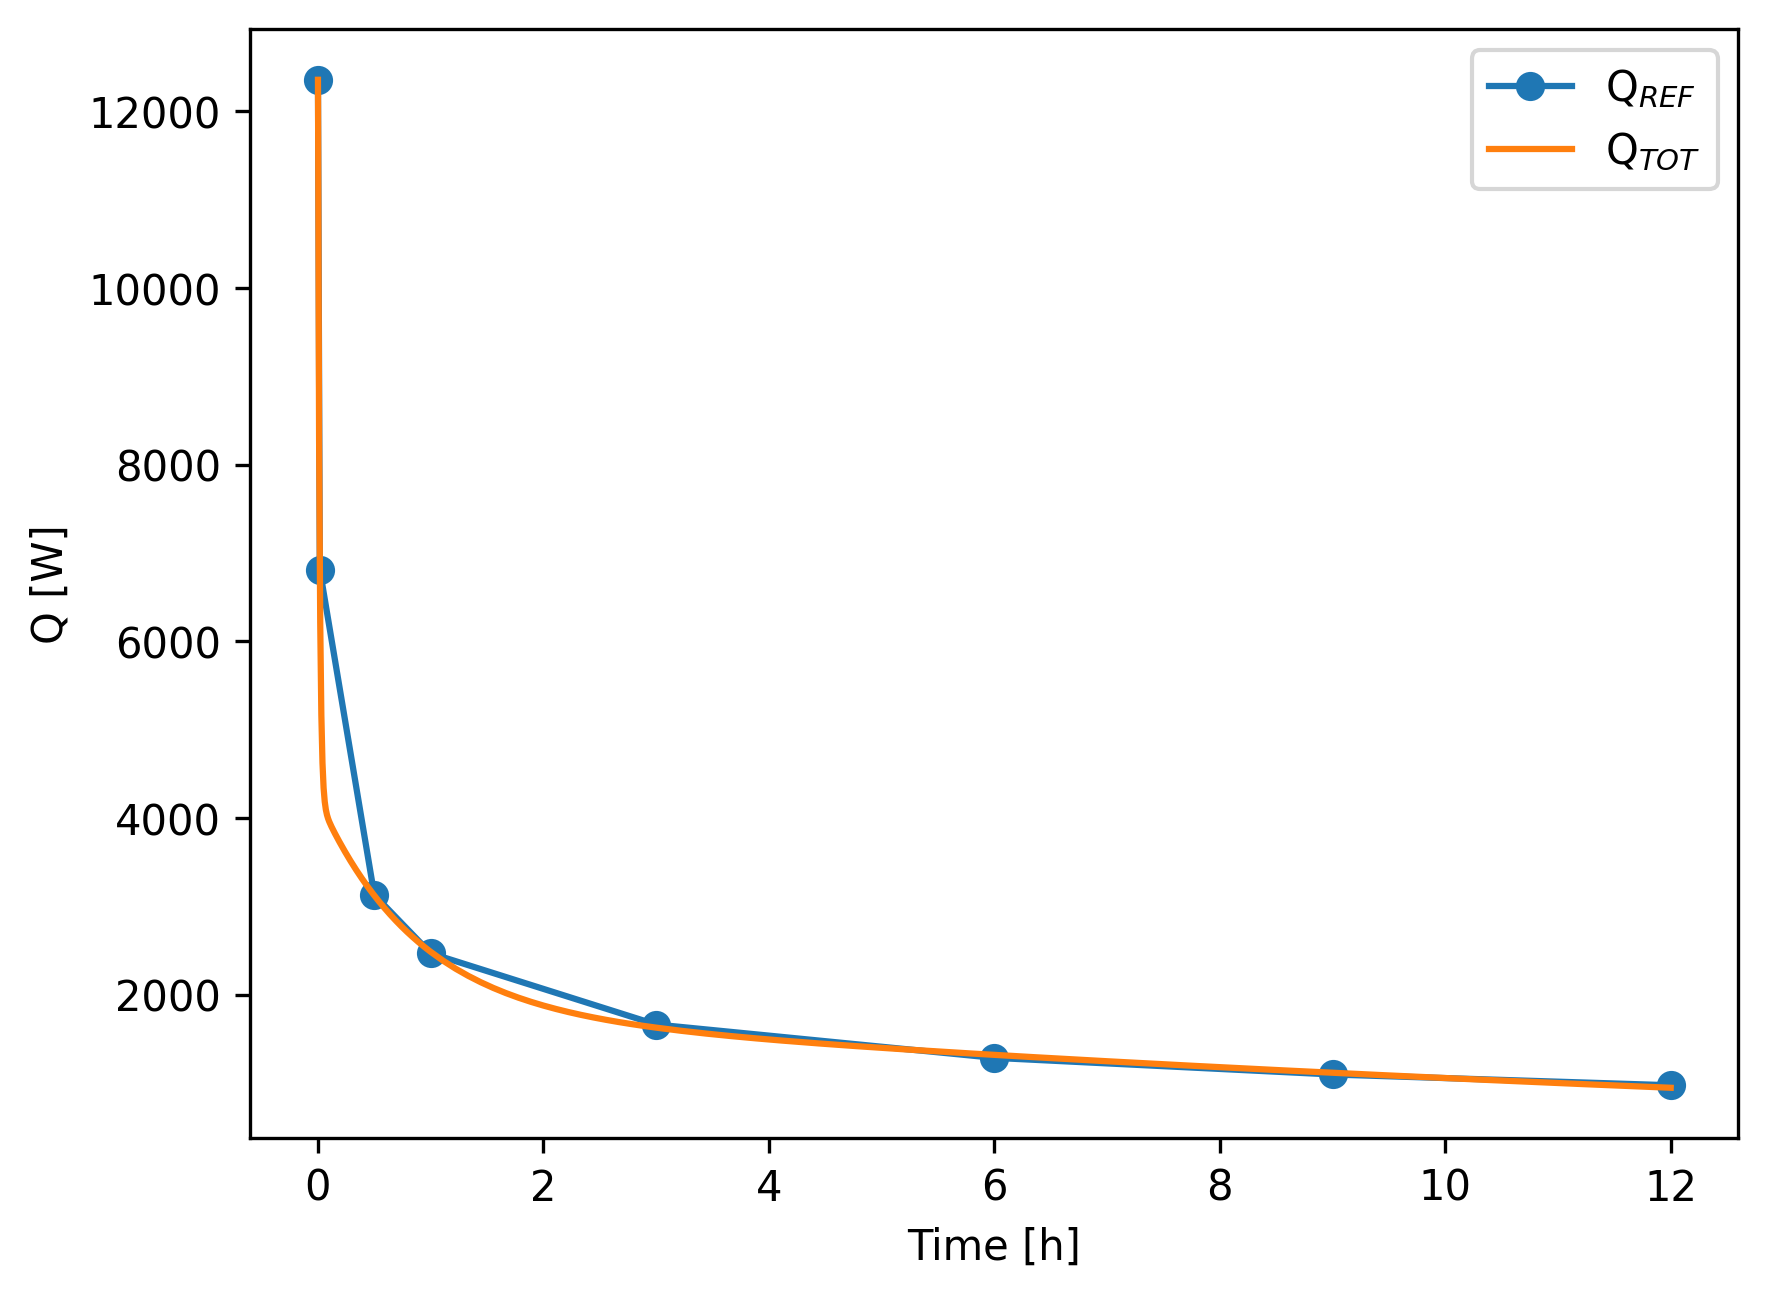
\includegraphics[width=0.45\linewidth]{figures/atr-U3Si2Al-deco-1}
    \hfill
    \caption{Delayed heating over time for ATR experiment of $U_3(20\%)Si_2/Al$.}
    \label{fig:modes-atr-2}
\end{figure}

% U3Si2Al - Trying to reproduce the material properties:
% U-92: 0.2 * 235.0439 + 0.8 * 238.0508
% Si-14: 0.92223 * 27.9769 + 0.04685 * 28.9765 + 0.03092 * 29.9738
% Al-13: 26.9815385
% aluminum,13,al,2698.0,225.94,921
% U3Si2:  3/5 * 237.4494 + 2/5 * 28.085475408 = 153.7038 g/mol
% % https://www.osti.gov/servlets/purl/1478507
% Cp = 120 J/mol-K = 120/153.7038 = 0.78072 J/g/K = 780.72 J/kg/K
% k = 8 W/m/K
% rho = 11.54 g/cm3
% 0.5*153.7038 + 0.5*26.9815385 = 90.34 g/mol
% wU = 153.7038/(153.7038 + 26.9815385) = 0.85
% wAl = 26.9815385/(153.7038 + 26.9815385) = 0.15
% rho_T = wU * rho_U + wAl * rho_Al = ??
% rho_T = rho_U + rho_Al = ??
% I coudln't reproduce them ...
The material properties of $U_3Si_2/Al$ were calculated using \cite{U3Si2Al} as reference.
The molecular weight is 90.32 g/mol, the density is 5660 kg/m$^3$, the heat capacity is 1290 J/kg/K, and the thermal conductivity is 84 W/m/K.
Figure \ref{fig:atr-u3si2al} shows the evolution of the highest temperature in the capsule for the experiment of $U_3Si_2/Al$.
The capsule reaches the maximum temperature of 1047.6 K at 1200 seconds, and it is located in the capsule's inner wall at the middle of the total height.
The temperature in the capsule shows a similar behavior than for the experiment of aluminum.
The temperature exhibits quick and slow responses, corresponding to the smallest and largest decay times in the volumetric heat.
Hence, the temperature increases rapidly from the initial condition, and after reaching the maximum, it decays slowly.
% The simulations used an fixed time step between 8$\times$10$^{-4}$.

\begin{figure}[htbp!] %or H
    \centering
    \includegraphics[width=0.45\linewidth]{figures/atr-U3Si2Al}
    \hfill
    \caption{Time evolution of the highest temperature in the capsule for ATR experiment of $U_3Si_2/Al$.}
    \label{fig:atr-u3si2al}
\end{figure}

% data-based: classification
The next step is the creation of the data-based model.
This step requires the repeated run of the thermal-fluids model described above to create the training and testing data.
The data-based model relies on the classification strategy described in Section \ref{sec:datapros} to predict the state of the experiment's capsule.
Based on the results from Section \ref{sec:sou_decomp}, the features of the model are: $\rho$, $c_p$, $k$, $q_{1,0}$, $q_{2,0}$, $q_{3,0}$, $\tau_1$, $\tau_2$, and $\tau_3$.

% MATERIAL DATA: rho, cp, k: in cfd/material_decomposition.ipynb
% SOURCE DATA: cfd/source_decomposition.ipynb
The material data ($\rho$, $c_p$, $k$) is generated assuming a multivariate normal distribution centered on real material data, which is shown in Appendix \ref{ap:mat_props}.
Based on the results from Section \ref{sec:syn-mat}, the use of synthetic material data wherein the variables are independent reduces the accuracy of the model.
Hence, using a multivariate normal distribution preserves a certain correlation between the thermal properties.
The synthetic data is generated using the \textit{multivariate\_normal} function from the \textit{NumPy} \textit{random} package.
This function takes a mean value and covariance.
The mean value is given by the real material data at which the normal distribution is centered.
The covariance is calculated using all the real material data, and it is down-scaled to 1\% of the original value to reduce the spread around each sample.
Figure \ref{fig:atr-syn-mats-1} shows some examples of synthetic material properties, showing the correlation between thermal properties.

\begin{figure}[htbp!] % or H
  \centering
  \begin{subfigure}[b]{0.49\textwidth}
    \centering
    \includegraphics[width=0.85\textwidth]{figures/syn-rho_k}
    \caption{Thermal conductivity vs. density.}
  \end{subfigure}
  \hfill
  \begin{subfigure}[b]{0.49\textwidth}
    \centering
    \includegraphics[width=0.85\textwidth]{figures/syn-rho_cp}
    \caption{Heat capacity vs. density.}
  \end{subfigure}
  \par
  \begin{subfigure}[b]{0.49\textwidth}
    \centering
    \includegraphics[width=0.85\textwidth]{figures/syn-k_cp}
    \caption{Heat capacity vs. thermal conductivity.}
  \end{subfigure}
  \caption{Synthetic material properties.}
  \label{fig:atr-syn-mats-1}
\end{figure}

The source data ($q_{i,0}$, $\tau_i$) is created using the delayed heating workflow on the material experiments shown in Appendix \ref{ap:mat_props_neut}.
Figure \ref{fig:atr-source1} shows the relationship $q_{i,0}$ vs. $\tau_i$ for all samples.
The samples exhibit three clusters based on the values of $\tau_i$, and they can be grouped into slow, intermediate, and fast response.
The synthetic source data was generated using the \textit{multivariate\_normal} function, assuming a normal distribution for $q_{i,0}$ and $\tau_i$ centered around each cluster's mean value.
Figure \ref{fig:atr-source2} shows each of the clusters with the original and the generated data.

\begin{figure}[htbp!] %or H
  \centering
  \includegraphics[width=0.45\linewidth]{figures/q0_vs_tau}
  \hfill
  \caption{Relationship between $q_{i,0}$ and $\tau_i$.}
  \label{fig:atr-source1}
\end{figure}

\begin{figure}[htbp!] % or H
  \centering
  \begin{subfigure}[b]{0.49\textwidth}
    \centering
    \includegraphics[width=0.85\textwidth]{figures/q0_vs_tau_cl2}
    \caption{Fast response constants.}
  \end{subfigure}
  \hfill
  \begin{subfigure}[b]{0.49\textwidth}
    \centering
    \includegraphics[width=0.85\textwidth]{figures/q0_vs_tau_cl3}
    \caption{Intermediate response constants.}
  \end{subfigure}
  \par
  \begin{subfigure}[b]{0.49\textwidth}
    \centering
    \includegraphics[width=0.85\textwidth]{figures/q0_vs_tau_cl1}
    \caption{Slow response constants.}
  \end{subfigure}
  \caption{Synthetic source data.}
  \label{fig:atr-source2}
\end{figure}

% Data
The combination of the synthetic material properties and source data creates 1227 samples, giving the input data $X$ the shape 1227 $\times$ 9.
The output data is generated by running the thermal-fluids model.
The simulation time was two hours (7200 seconds) after the accident.
Because the simulations utilized an adaptive time stepper, the outputs were adjusted to give them a fixed length by linear interpolation.
The interpolation was calculated for 100 points from 0 to 500 seconds and 101 points from 500 to 7200 seconds.
Consequently, the shape of the output data $Y$ was 1227 $\times$ 201.
Finally, the data is prepared using the scheme described in Figure \ref{fig:data-class}.

% Results
Table \ref{tab:results-atr} summarizes the main results of the classification problem for the testing dataset.
In terms of accuracy, KNN is the worst-performing method, and DT, FNN, and LogR are the best-performing methods.
All the methods show an accuracy higher than 0.95.
When focusing on the recall, KNN shows the worst performance with a value below 1.
All the rest of the methods show a recall of 1.
The last comparison metric is the model training time.
All the methods are trained quickly in under 1 second, except for FNN which took 4 seconds (excluding hyperparameter tuning).
Although several methods show a recall of 1, high recall is only good in combination with high accuracy.
Hence, the best performance is achieved by DT, FNN, and LogR.
Finally, Figure \ref{fig:atr-class-1} displays the confusion matrix for the KNN and the FNN cases.
The comparison of both results shows a clear improvement from KNN to FNN in the mislabeled samples.

% Table
\begin{table}[htbp!]
  \centering
  \caption{Performance metrics of the machine learning techniques for the classification problem.}
  \label{tab:results-atr}
  \begin{tabular}{lccc}
    \toprule
    Method & Accuracy & Recall & Train Time [sec] \\
    \midrule
    DT      & 1.0000 & 1.0000 & $<$1 \\
    FNN     & 1.0000 & 1.0000 & 4 \\
    KNN     & 0.9593 & 0.9610 & $<$1 \\
    LogR    & 1.0000 & 1.0000 & $<$1 \\
    RF      & 0.9959 & 1.0000 & $<$1 \\
    SVM     & 0.9837 & 1.0000 & $<$1 \\
    \bottomrule
  \end{tabular}
\end{table}

\begin{figure}[htbp!] %or H
  \centering
  \includegraphics[width=0.45\linewidth]{figures/atr-classification_cnfm}
  \hfill
  \caption{Confusion matrix for the KNN (top) and FNN (bottom) cases. The labels 1/0 represent \textit{melt}/\textit{does not melt}.}
  \label{fig:atr-class-1}
\end{figure}


\section{Conclusions}

% Intro
The prediction of the temperature in selected locations of a nuclear reactor is of paramount importance to ensure component integrity during a transient.
This work focuses on the safety analysis of research reactor experiments.
This chapter studied the response of a simplified model of a experiment and an ATR experiment to the channel draining event, where the experiments are left uncovered and the natural circulation of air cools them down.

Additionally, this chapter investigated the applicability of data-based modeling and machine learning to forecast the state of an experiment's capsule during the accident.
The study focused first on the simplified model experiment to guide the choice of a method for the ATR experiment.
The study considered two different strategies.
The first strategy focused only on answering whether the capsule melted or not.
The second strategy added the answer to the question of when the capsule melted.
Both strategies obtained satisfactory results in terms of accuracy and recall.
The melting time prediction had large maximum relative errors, in the order of 30 to 50\%.
Nevertheless, the different methods showed low mean relative errors, showing an overall successful performance.
In general, this simplified model proved that data-based modeling enables the quick determination of whether the capsule melts or not for any given irradiated material provided its thermal properties are known.

Further analysis of the delayed heating results in Chapter \ref{ch:delayedheat} showed that the application of the data-based modeling to the ATR experiment required a slight modification to properly capture the heat evolution in the experiment.
Consequently, the delayed heating in the ATR experiment was modeled as the linear combination of three exponential decay functions.
This chapter also described the assumptions and simplifications considered in the making of the thermal-fluids model of the ATR experiment.
Two results were shown.
First, for an experiment of aluminum, and second, for an experiment of $U_3Si_2/Al$.
While the first case showed temperatures lower than the melting temperature, the second case showed a temperature exceeding 1000 K, which results in the capsule melting.

Finally, the repeated run of the thermal-fluids model with both synthetic material and source data generates data for the training and testing of a data-based model of the ATR experiment.
The results of the testing dataset show high accuracy and recall for most of the machine learning algorithms.
These results prove that this work's proposed method relying on data-based modeling decreases the computational expense and enables the fast determination of the accident outcome.

% ABOUT THE DECOMPOSITION OF THE PROBLEM INTO 3 FOR THE TEMPERATURE
% This section has a twofold purpose.
% First, to establish a decomposition strategy for the delayed heating over time.
% And second, to study if the temperature evolution of an experiment can be calculated as a linear combination of the temperature evolution of experiments using as sources the individual terms of the decomposed original source.

% % Second part
% The next step is to determine if the temperature of the experiment could be calculated from the temperature of experiments using as sources the individual terms of the original source.
% % Math justification
% The heat conduction equation solves the temperature in the solid with a time dependent-source $q'''_i(t)$
% \begin{align}
% & \rho cp \frac{\partial}{\partial t} T_i = \nabla^2 T_i + q'''_i \\
% \end{align}

% Let's add together the equations for sources with two terms:
% \begin{align}
% & \rho cp \frac{\partial}{\partial t}(T_1 + T_2) = \nabla^2 (T_1 + T_2) + q'''_1 + q'''_2 \label{eq:heat2} \\
% \end{align}
% where $q'''_1$ and $q'''_2$ compose the reference source $q'''_{REF}$.

% We consider that the reference temperature can be computed as a linear combination of the temperatures of the individual sources
% \begin{align}
% & \tilde{T}_{REF} = \tilde{T}_1 + \tilde{T}_2  \\
% & \tilde{T}_i = (T_i - T_{SS})/T_{SS}
% \end{align}
% where $\tilde{T}_i$ is the non-dimensional temperature, and $T_{SS}$ the steady-state value, and in this case the initial condition.
% Re-arranging the terms yields 
% \begin{align}
% T_{REF} = T_1 + T_2 - T_{SS}
% \end{align}
% and inserting this into Equation \ref{eq:heat2} produces the heat conduction equation for the reference case 
% \begin{align}
% & \rho cp \frac{\partial}{\partial t} T_{REF} = \nabla^2 T_{REF} + q'''_{REF} \\
% \end{align}
% proving that the solution of the individual cases can produced the solution of the reference case.

% % & \tilde{T}_{REF} = \tilde{T}_1 + \tilde{T}_2
% % & \tilde{T}_i = (T_i - T_{SS})/T_{SS}
% % (T_{REF} - T_{SS})/T_{SS} = (T_1 - T_{SS})/T_{SS} + (T_2 - T_{SS})/T_{SS}
% % T_{REF} - T_{SS} = (T_1 - T_{SS}) + (T_2 - T_{SS})
% % T_{REF} = (T_1 - T_{SS}) + (T_2 - T_{SS}) + T_{SS}
% % T_{REF} = T_1 + T_2 - T_{SS}

% The demonstration is complete once we consider the boundary conditions at the interfaces, which are temperature and heat flux continuity.
% As the initial condition is independent from the spatial coordinates, the separation of the non-dimensional reference temperature into modes is still valid.  

% % Then we just need to solve the interface BCs, which are temperature and heat flux continuity.
% % T_{REF,s} = T_{REF,f}
% % k_s \frac{\partial}{\partial n} T_{REF,s} = k_f \frac{\partial}{\partial n} T_{REF,f}
% % And the scaling applies to both T_{REF,s} and T_{REF,f}.

% % T_{REF,s} = T_{1,s} + T_{2,s} - T_{SS}
% % T_{REF,f} = T_{1,f} + T_{2,f} - T_{SS}
% % T_{1,s} + T_{2,s} - T_{SS} = T_{1,f} + T_{2,f} - T_{SS}
% % T_{1,s} = T_{1,f}
% % T_{2,s} = T_{2,f}

% % And the same for the heat flux.

% The following exercise intends to numerically verify this conclusion.
% Three different cases were considered:
% % Verification Examples
% \begin{enumerate} % Need to represent this with letters instead of numbers
% \item $q_{REF} = 10^9 exp( -t / 0.2) + 5 \times 10^8 exp( -t / 4)$
% \item $q_{REF} = 2 \times 10^9 exp( -t / 1) + 3 \times 10^8 exp( -t / 10)$
% \item $q_{REF} = 10^9 exp( -t / 4) + 4 \times 10^8 exp( -t / 20)$
% \begin{enumerate}

% Figure \ref{fig:modes-T} displays the results for the verification examples, where $T_{TOT}$ corresponds to the calculated temperature.
% There is good agreement between the calculated and reference results, demonstrating that this method is suitable for our purposes.

% \begin{figure}[htbp!] % or H
%   \centering
%   \begin{subfigure}[b]{0.48\textwidth}
%     \centering
%     \includegraphics[width=0.98\textwidth]{figures/modes1-T}
%     \caption{}
%   \end{subfigure}
%   \hfill
%   \begin{subfigure}[b]{0.48\textwidth}
%     \centering
%     \includegraphics[width=0.98\textwidth]{figures/modes2-T}
%     \caption{}
%   \end{subfigure}
%   \hfill
%   \begin{subfigure}[b]{0.48\textwidth}
%     \centering
%     \includegraphics[width=0.98\textwidth]{figures/modes3-T}
%     \caption{}
%   \end{subfigure}
%   \caption{Verification examples of source decomposition.}
%   \label{fig:modes-T}
% \end{figure}

% The last piece of the analysis should consider the addition of the data-based model.
% So far, this work has used two data-based modeling approaches, one using classification algorithms and the other relying on the temperature evolution prediction.
% For the second approach, the application of the source decomposition is straight forward as the solution of the approach is the temperature at each time step.
% For the first approach, additional considerations are necessary.
% ...

% Also, this method succeeds here as we are not including radiation.
% Once we do, this method remains as an approximation.

% ML should predict max T (regression) instead of melt/does not (classification)
% Take random combinations of samples (all should have the same material properties, but different decay curves).
% Sample 1 --> Max T Prediction 1
% Sample 2 --> Max T Prediction 2
% Sample 3 --> Max T Prediction 3
%              ------------------
%              Tot Temp --> Melt/Does Not

% Add together q1 + q2 + q3 --> run OF to calculate max T
% Use unseen material data
% 1 case that melts, 1 case that does not melt


% % Conclusions
% These results prove
% that the sources can be decomposed into different exponential decay functions,
% that the temperature of a case using a non-pure exponential decay can be computed as a combination of the temperature of the independent source modes,
% that the data-based models can be trained for pure exponential decay functions, and the outcome determined as a linear combination of the predictions for the independent modes.
